

\documentclass[a4paper, 12pt, twoside]{toptesi}
\usepackage{epsfig}
\usepackage{amsmath, amsthm, amsfonts}
%\usepackage{psfrag}
\usepackage[italian]{babel}
\usepackage[english]{babel}
\usepackage{tikz}
\usepackage{caption}
\usepackage{graphicx}
\usepackage{signalflowdiagram}
\usepackage{gnuplot-lua-tikz}
%\usepackage[urw-garamond]{mathdesign}
\usepackage{microtype}
\usepackage{listings}
%\usepackage[ansinew]{inputenc}
\usepackage{subfig}
%\usepackage{showkeys}
\usepackage[T1]{fontenc}


\theoremstyle{plain}
\newtheorem{Theorem}{Theorem}[section]
\theoremstyle{definition}
\newtheorem{Def}{Definition}[section]

\DeclareMathSymbol{\virgola}{\mathpunct}{letters}{"3B}
\DeclareMathSymbol{\decimalcomma}{\mathord}{letters}{"3B}
\DeclareMathOperator{\im}{\mathrm{j\mathstrut}}
%\DeclareMathOperator{\mod}{\mathrm{j\mathstrut}}
\newcommand{\vet}[1]{\mathbf{#1}}
%\newcommand{\eqref}[1]{(\ref{#1})}
\newcommand{\figref}[1]{Figure \ref{#1}}
\newcommand{\tbref}[1]{Table \ref{#1}}
\newcommand{\secref}[1]{Section \ref{#1}}
\newcommand{\bch}[2]{$\mathrm{BCH(#1\virgola #2)}$}
\bibliographystyle{plain}

\lstset{ %default parameters
            basicstyle=\tiny,
			language=C,
			tabsize=2,
            showspaces=false,
            showstringspaces=false,
            %frame=tb,
            captionpos=t,
            abovecaptionskip=2\baselineskip,
            framexbottommargin=\baselineskip
			}

%\usepackage{fancyhdr}

%\renewcommand{\chaptermark}[1]{%
%\markboth{\MakeupperCase{\chaptername
%\ \thechapter\#1{}}}}

%\titolo{Studi di tricotetratomia applicata}
%\sottotitolo{Cosa succede quando si spacca un capello in quattro}
%\candidata{Maria Chiomafolta}
%\relatore{prof.\ Piero Scapigliati}
%\sedutadilaurea{Maggio 2006}

\includeonly{%
preliminari,%
riassunto,%
cap1,%
cap2,%
cap3,%
cap4,%
cap5,%
cap6,%
conclusioni, %
basic,%
bibliografy,%
}

\begin{document}
\frontespizio


\sommario

Il lavoro svolto nell'ambito di questa tesi ha avuto l'obiettivo di consentire la progettazione di un dispositivo di trasmissione di bordo per comunicazioni via satellite, fondato sullo standard DVB-S2, contribuendo ad una particolare sezione del progetto. Si sono analizzate e impiegate le pi� moderne tecniche nel campo della modulazione e codifica, viste le prestazioni altamente sfidanti da raggiungere nel particolare scenario applicativo.

In ogni sistema di comunicazione la scelta e il progetto degli schemi di modulazione e codifica ha come finalit� quella di trasmettere i dati in maniera sufficientemente affidabile per il tipo di applicazione richiesta, facendo al tempo stesso un uso efficiente delle risorse disponibili (banda, potenza, e, in particolare nelle comunicazioni via satellite, peso ed ingombro delle apparecchiature).

Nel 1948, Claude E. Shannon definisce e quantifica l'informazione, riuscendo inoltre a dimostrare che, per una qualsivoglia velocit� di trasmissione minore o uguale a un cardinale parametro chiamato capacit� di canale, esiste uno schema di codifica in grado di ottenere una probabilit� d'errore arbitrariamente piccola, garantendo cos� una trasmissione completamente affidabile dei dati. Purtroppo Shannon nel suo teorema non d� alcuna indicazione su come poter trovare questi schemi di codifica. Shannon dimostra tuttavia che codici lunghi scelti casualmente assicurano una bassa probabilit� d'errore media. Purtroppo una diretta realizzazione dei codici suddetti porta ad avere una complessit� di decodifica molto alta. Dal 1948, quindi, l'impegno degli ingegneri delle telecomunicazioni si concentra sullo sviluppo di schemi realizzabili di modulazione e codifica, che si avvicinino alle prestazioni limite. Nonostante l'iniziale pessimismo (si pensi al motto \emph{``good codes are messy''} che circolava tra gli studiosi di teoria dei codici), il problema viene risolto almeno per il caso di maggior interesse e importanza, il canale lineare gaussiano bianco (AWGN, \emph{Additive  White Gaussian Noise}).

Nel 1980, poi, la migliore comprensione del significato del teorema di Shannon porta a una revisione del paradigma utilizzato sino ad allora nel campo delle modulazioni e della codifica. Queste due discipline, che prima di questo momento si sviluppavano indipendentemente, incominciano a diventare rigidamente collegate. Parallelamente, l'esigenza di ottenere alte efficienze spettrali fa aumentare la cardinalit� delle modulazioni (il numero delle forma d'onda impiegate in ogni simbolo); nel frattempo, vengono ideati codici a correzione d'errore ancora pi� efficaci. In tale contesto il lavoro di Ungerboek sancisce l'arrivo dei codici TCM (\emph{Trellis Coded Modulation}), rendendo chiari i vantaggi del trattare modulazione e codifica come una entit� singola.
Inoltre, vari schemi pubblicati in letteratura dimostrano che turbo codici (una tecnica di codifica introdotta nel 1993 da Claude Berrou) e TCM possono essere utilizzati con profitto congiuntamente. Tuttavia i turbo codici dovrebbero essere progettati ad hoc per ogni singola modulazione, una soluzione impraticabile per sistemi che adottano diverse costellazioni. La soluzione di questo problema prende il nome di \emph{Bit Interleaved Coding Modulation} (BICM), tecnica grazie alla quale � possibile ottenere dei risultati eccellenti impiegando una singola soluzione di codifica per tutte le modulazioni previste. Questa grande flessibilit� rende le BICM commercialmente appetibili per sistemi comunicazione satellitari a banda larga di tipo adattativo (\emph{Adaptive Coding Modulation}, ACM) che necessitano di  un ampio ventaglio di efficienze spettrali. Appartengono alle soluzioni ACM anche lo standard ETSI DVB-S2 e la soluzione MHOMS in via di standardizzazione nel CCSDS (\emph{Consultive Committee for Space Data Systems}).

Il recente standard DVB-S2, successivo al gi� consolidato DVB-S, utilizza gran parte delle pi� recenti e innovative tecniche nel campo della codifica di canale e delle modulazioni congiuntamente a modulazioni ad alta cardinalit�, come la 16APSK e la 32APSK. Il `motore' (ovvero l'elemento essenziale) della codifica di canale � composto da un codice LDPC concatenato a un BCH per limitarne il tipico calo delle prestazioni ad altri rapporti segnali rumore, che prende il nome di \emph{error floor}.  Questa scelta garantisce delle prestazioni (riferendoci alla sola modulazione e codifica) tra 0,6-1,2 dB dal limite di Shannon. Oltre a ci�, il DVB-S2, offrendo un gran numero di modalit� operative e quindi un ampio raggio di efficienze di banda per la trasmissione del segnale, � adatto a numerose tipologie di missione spaziale. Le caratteristiche di alta regolarit� e periodicit� dell'LDPC, poi, garantiscono una complessit� ragionevole sia in fase di codifica che in fase di decodifica.

Dopo una parte introduttiva dedicata allo studio delle principali caratteristiche ed applicazioni delle comunicazioni satellitari, quali i servizi di diffusione del segnale televisivo, telerilevamento, raccolta dei dati, etc., si descrivono i blocchi funzionali della sezione di trasmissione del DVB-S2, che come gi� accennato, raccoglie gran parte degli aspetti pi� innovativi nel campo delle modulazioni e codifica di canale. Si mette inoltre in evidenza come la tecnica ACM, ossia di modulazione e codifica adattativa, possa garantire un pi� alto \emph{throughput}, una maggiore disponibilit� del servizio (specie se confrontata con quella ottenuta adoperando modulazione e codifica costanti (CCM)),  una maggiore efficienza e ottimizzazione delle risorse disponibili a bordo del satellite.
Si passa quindi alla revisione critica della codifica di canale (FEC, \emph{Forward Error Correction}) del DVB-S2. Dopo una breve descrizione dei principali criteri di costruzione dei codici BCH, vengono illustrate le caratteristiche del particolare codice BCH adoperato nello standard DVB-S2, per poi passare alla descrizione dei codici LDPC; cercando di dare una giustificazione della loro ``rinascita'', nonch� di spiegarne la struttura, i metodi e gli algoritmi di codifica, e specialmente la loro decodifica iterativa a ``passaggio di messaggi''.

La parte centrale della tesi � invece dedicata allo studio di algoritmi di codifica efficienti e veloci dei codici BCH e alla loro realizzazione in hardware. Dopo una fase preliminare di analisi del tradizionale algoritmo di codifica per il codice BCH sistematico (quale quello utilizzato dal DVB-S2), si descrivono le possibili architetture seriali capaci di realizzare il metodo di codifica, analizzandone pregi e difetti in vista della successiva realizzazione in hardware. Queste semplici architetture sono intrinsecamente seriali e quindi lente; esse sono chiamate Linear Feedback Shift Register (LFSR) e realizzano la divisione per il polinomio generatore del codice. Tale metodo di codifica � tipico della famiglia dei codici ciclici a cui appartengono i codici BCH. Dal punto di vista hardware, la lunghezza delle parole di codice (previste dal DVB-S2), i vincoli di frequenza imposti dell'analisi globale della sezione di trasmissione e la definizione dell'interfaccia con il codificatore LDPC che ha un ingresso necessariamente parallelo, impongono lo sviluppo di un modello di codificatore BCH a sezioni multiple che risponda alle specifiche di velocit� e sia agevolmente integrabile con l'intera sezione di trasmissione del DVB-S2. La descrizione matematica della versione dell'algoritmo di codifica parallelo (ottenuta per mezzo delle equazioni di stato) e, in particolare, le fortunate propriet� di regolarit� della matrice di transizione di stato \(\vet A\) ricavata dal modello del sistema conducono ad una realizzazione particolarmente efficiente del codificatore BCH. Oltretutto, l'algebra binaria usata nelle operazioni di codifica, per cui le operazioni di somma vengono direttamente realizzate per mezzo di porte XOR mentre quelle di moltiplicazione per mezzo di AND,  riduce drasticamente il carico computazionale e, specialmente, il contributo di ritardo delle operazioni elementari ai cammini critici del grafo della elaborazione algoritmica per la frequenza di clock da raggiungersi.

La scelta dell'architettura hardware e del suo livello di parallelismo (scelta pari a 8 rami paralleli, sebbene il modello matematico sviluppato sia del tutto generale e consenta di modificare a piacimento tale parametro progettuale) � stata dettata, come gi� detto, non solo dai vincoli imposti dalla sezione di trasmissione realizzata, ma specialmente dalla esigenza di disporre di un codificatore in grado di operare in modalit� ACM, ossia in accordo con le raccomandazioni dello standard ETSI DVB-S2, secondo il quale le modalit� di modulazioni e codifica possono variare da una trama all'altra. Ci� comporta anche la memorizzazione di alcuni coefficienti di tutte le matrici \(\vet A^p\) e \(\vet B_p\) (dove \(\vet B_p\) � la matrice trasferimento ingresso-stato) associate alle varie capacit� correttive del codice BCH in delle tabelle di riferimento o \emph{Look Up Table} (LUT). L'architettura hardware realizzata in TAS-I comprende un registro a 192 celle (\emph{Flip Flop}), 192 reti combinatorie d'ingresso e 192 reti combinatorie d'uscita, pilotate opportunamente dai coefficienti (precedentemente calcolati) memorizzati nelle LUT, e alcuni sommatori, che, come gi� osservato, sono delle porte XOR a due ingressi. Le reti combinatorie sono in realt� delle porte XOR a otto ingressi, la cui abilitazione � pilotata (per mezzo di porte AND a 2 ingressi) dai coefficienti precalcolati e memorizzati nelle LUT. Il poter pilotare le reti combinatorie per mezzo di alcune LUT rende possibile la codifica, lasciando ovviamente intatta l'architettura ideata, per tutte le modalit� operative previste (modulazione e codifica BCH-LDPC) dallo standard ETSI DVB-S2. Si tratta semplicemente di inibire le prime 32 o 64 coppie di reti combinatorie (quelle che operano sugli ingressi e quelle che agiscono sul bus di uscita) a seconda della capacit� correttiva del codice BCH, ossia 10 e 8.

Un capitolo della tesi � dedicato alla descrizione del lavoro di simulazione svolto in linguaggio C/C++ delle architetture e degli algoritmi impiegati allo scopo di fornire supporto e dati di riferimento per la di verifica funzionale ai progettisti VLSI (\emph{Very Large Scale Integration}) nella sintesi del progetto mediante linguaggio di progettazione digitale VHDL \english{(\emph{Very high speed integrated circuits Hardware Description Language})}, e nella successiva verifica dei risultati prodotti dal modello descritto. Tutto questo, per�, non prima di aver verificato mediante un adeguato numero di simulazioni in linguaggio C la corretta generazione delle parole di codice (tramite un programma di rivelazione degli errori) nonch� l'effettiva capacit� correttiva del codice, attraverso l'inserzione di errori pseudocasuali  e successiva elaborazione di decodifica. Una parte del capitolo � poi dedicata all'algoritmo di decodifica impiegato, quello di Berlekamp-Massey che consente di evitare la costosa operazione d'inversione della matrice, sfruttando la relazione lineare (del tipo LFSR) tra i valori di sindrome del codice e i coefficienti di un polinomio grazie al quale � possibile individuare le posizioni degli errori occorsi durante la trasmissione. Tale polinomio � chiamato per questo motivo polinomio di identificazione della collocazione degli errori. Dato che le operazioni in fase di decodifica, compresa la \emph{error detection}, devono essere effettuate nel campo di Galois in cui giacciono le radici del polinomio generatore, � stata prestata particolare attenzione allo studio della struttura del codice BCH previsto dal DVB-S2 (completando le riduttive informazioni fornite dallo standard e concludendo che si tratta di un codice primitivo e shortened , ossia pi� corto rispetto alla sua lunghezza ``naturale'') e alla conseguente determinazione e costruzione di tabelle (del campo finito) ausiliarie per poter effettuare tutte le operazioni necessarie durante le operazioni di decodifica.

Infine, l'ultima parte della tesi si spinge a mostrare anche i risultati sinora raggiunti delle fasi di collaudo in laboratorio realizzate sull'intera sezione di trasmissione del sistema DVB-S2 sviluppata da TAS-I. Il progetto hardware � attualmente in corso di verifica mediante l'uso di una scheda di prototipazione Altera fondata su FPGA (\emph{Field Programmable Gate Array}) EP180 Stratix II. Non si � ancora giunti alla prova BER \emph{end-to-end}, ma si sono effettuate verifiche delle prestazioni della sezione di modulazione ad  elevata cardinalit�. Nella descrizione si illustra brevemente l'architettura e i blocchi della intera sezione di trasmissione, vengono mostrati i risultati ottenuti attraverso un VSA (\emph{Vector Signal Analyzer}) a banda larga, in grado di demodulare il segnale, interconnesso ad un oscilloscopio, entrambi prodotti Agilent. Le prestazioni della sezione di trasmissione sono state valutate attraverso l'analisi statistica degli errori di ampiezza e di fase (effettuata dal VSA). Tra elementi di innovazione associati alle elevate velocit� di simbolo da raggiungersi, si � affrontato anche il problema della correzione della distorsione d'ampiezza del convertitore digitale-analogico (DAC, \emph{Digital to Analog Converter}). Le misure effettuate mostrano infatti l'importanza del filtro di precompensazione quando le velocit� di trasmissione dei dati sono pi� elevate.

\italiano
\ringraziamenti

Ringrazio il prof.~Roberto Garello che mi ha dato la possibilit�, mettendomi in contatto con l'ing.~Domenico Giancristofaro, di svolgere l'attivit� di tesi a L'Aquila.

Desidero ringraziare la Thales Alenia Space Italia di L'Aquila e, segnatamente, il suo reparto di architetture e algoritmi, che mi ha messo a disposizione tutti gli strumenti e il materiale necessari allo svolgimento e completamento della mia attivit� di tesi.

Sono grato all'ing. Domenico Giancristofaro, che, nonostante i numerosi impegni, mi ha seguito con costanza e pazienza durante lo svolgimento della mia attivit� in TAS-I.

Infine, un ultimo ringraziamento agli ingegneri Cinzia Moca e Massimo Fonte, che mi hanno fornito degli ottimi spunti e consigli, utili allo svolgimento della mia attivit� e alla redazione della tesi.



%In communication systems, the coding and modulation problem represents the real essence of the reliable communications. The pioneer of the analysis of theoretical aspects of such a problem was Claude E.Shannon, who was able to define mathematically the information and hence to show how it is connected to the problem of establishing a reliable communications between 2 or more points. However, the well known Shannon limit and results related to states the existence of a way to virtually transmit messages with a zero error probability.
%In ogni sistema di comunicazione la scelta e il progetto degli schemi di modulazione e codifica ha come finalit� quella di trasmettere i dati in maniera sufficientemente affidabile per il tipo di applicazione richiesta, facendo un uso al tempo stesso efficiente delle risorse (banda, energia, peso, ingombro delle apparecchiature) disponibili.
%Nel 1948, Claude E.Shannon definisce e quantifica l'informazione, riuscendo inoltre a dimostrare che, per un qualche rate di trasmissione minore o uguale a un parametro chiamato capacit� di canale, esiste uno schema di codifica in grado di ottenere una probabilit� d'errore arbitrariamente piccola, garantendo cos� una trasmissione completamente affidabile dei dati. Purtroppo Shannon nel suo teorema non d� alcuna indicazione su come poter trovare questi schemi di codifica. Inoltre sappiamo che i codici lunghi scelti casualmente assicurano una bassa probabilit� d'errore media. Tuttavia una diretta implementazione dei codici suddetti porta ad avere una complessit� di decodifica molto alta. Dal 1948, quindi, le forze degli ingegneri delle telecomunicazioni si concentrano sullo sviluppo di schemi realizzabili di modulazione e codifica, che si avvicinino alle prestazioni limite. Nonostante l'iniziale pessimismo, il problema viene risolto almeno per il caso di maggior interesse e importanza, il canale lineare gaussiano bianco.
%Nel 1980, poi, la migliore comprensione del significato del teorema di Shannon porta a una revisione del paradigma utilizzato finora nel campo delle modulazioni e della codifica. Queste due discipline, che prima di questo momento si sviluppavano indipendentemente, incominciano a  diventare comunicanti. Parallelamente, l'esigenza di ottenere alte efficienze spettrali fa aumentare la cardinalit� delle modulazioni e, se da un lato, questo obiettivo viene centrato, dall'altro, vengono sviluppati codici a correzione d'errore ancora pi� efficaci. Infine, con il lavoro di Ungerboek e l'arrivo dei codici TCM (Trellis Coded Modulation), diventa chiaro che modulazioni e codifica dovrebbero essere trattate come una entit� singola.
%Inoltre,  vari schemi pubblicati in letteratura dimostrano che Turbo Codici e TCM possono essere utilizzati con profitto congiuntamente. Tuttavia i Turbo Codici possono essere progettati profittevolmente per una data modulazione, una soluzione impraticabile per sistemi che supportano pi� costellazioni. La soluzione di questo problema prende il nome di Bit Interleaved Coding Modulation (BICM), tecnica grazie alla quale � possibile ottenere dei risultati eccellenti (con codici standard, ossia non ottimizzati per una data modulazione)  e che ha l'intrinseco vantaggio di essere utilizzata per una moltitudine di modulazioni. Questa grande flessibilit� rende lo sviluppo di questa tecnica una caratteristica commercialmente appetibile per sistemi comunicazione satellitari a banda larga che abbisognano di  un ampio ventaglio di efficienze spettrali, come il DVB-S2.
%Il recente standard, successivo al gi� consolidato DVB-S, utilizza gran parte delle pi� recenti e innovative tecniche nel campo della codifica di canale e delle modulazioni. Il motore della codifica di canale � composto da un codice LDPC concatenato a un BCH per limitarne l'inevitabile calo delle prestazioni ad altri rapporti segnali rumore, che prende il nome di error floor.  Questa scelta garantisce delle prestazioni tra 0,6-1,2 dB dal limite di Shannon. Oltre a ci�, il DVB-S2 � in grado praticamente di operare su qualsiasi tipo di trasponder, offrendo un gran numero di modalit� operative e quindi un ampio raggio di efficienze in banda per la trasmissione del segnale. Le caratteristiche di alta regolarit� e periodicit� dell'LDPC, poi, garantiscono una complessit� ragionevole sia in fase di codifica che in fase di decodifica.



\indici





\italiano

\chapter{Riassunto}

\section{Applicazioni e caratteristiche delle comunicazioni satellitari}

Le comunicazioni satellitari rivestono un ruolo molto importante in applicazioni che potremmo definire di nicchia o altamente strategiche quali:

\begin{itemize}
\item 	La trasmissione e diffusione di dati multimediali su vaste aree geografiche a bassa densit� di popolazione, dove per l'appunto � sconveniente investire in infrastrutture di reti di comunicazione.
\item 	Le comunicazioni marittime (ad esempio Inmarsat) e i sistemi di radionavigazione, questi ultimi in particolare si stanno largamente diffondendo tra i prodotti consumer (si pensi ai noti navigatori satellitari TomTom per autoveicoli).
\item 	Diffusione della TV via satellite: � spesso economicamente pi� conveniente coprire una vasta area geografica attraverso satelliti piuttosto che attraverso una grossa rete di stazioni locali.
\item 	Telerilevamento e osservazione della Terra, settore altamente strategico sia per applicazioni militari sia per applicazioni civili.
\end{itemize}

In generale tutti questi tipi d'applicazione richiedono un alto \emph{bit rate}. Tuttavia le risorse a bordo dei satelliti sono preziose e limitate: questo spiega l'alto interesse da parte delle industrie a promuovere la ricerca nel campo delle modulazioni e della codifica canale in modo da ottenere delle prestazioni il pi� possibile vicine a quelle limite.

Le comunicazioni satellitari per l'osservazione della Terra e le Telecomunicazioni sono quindi caratterizzate dall'esigenza di ottenere un alto throughput ed efficienze in banda e potenza molto alte. Inoltre, la banda disponibile e i requisiti sulla velocit� di segnalazione e sul rapporto segnale rumore possono variare sensibilmente a seconda dell'applicazione e della specifica missione spaziale. Per questo motivo un'unit� modem sufficientemente flessibile da poter essere utilizzata per un numero elevato di missioni e applicazioni dovrebbe avere le seguenti peculiarit�:

\begin{itemize}
\item 	Regolazione della velocit� di trasmissione e della larghezza di banda
\item 		Prestazioni molto vicine (a un 1 dB massimo) dal limite di Shannon, rispetto al tipo di modulazione e codifica utilizzate
\item 	Utilizzo efficiente delle risorse hardware ed energetiche a bordo per l'acquisizione e l'elaborazione dei dati
\end{itemize}
Il sistema di modulazione e codifica adottato dal recente standard per le comunicazioni satellitari  DVB-S2, cos� come MOHMS, un innovativo modem ad alto ordine di modulazione e alte prestazioni sviluppato da TAS-I e finanziato dall'European Space Agency (ESA), � cos� vicino alle prestazioni limite (Shannon) da poter rappresentare una solida soluzione tecnologica per molti anni a venire.

\subsection{Osservazione della Terra e telerilevamento}

Come gi� accennato, i satelliti ricoprono un ruolo chiave in applicazioni (civili e militari) per cui � richiesta la copertura di vaste aree di territorio a bassa densit� di popolazione (per esempio, oceani, deserti, zone polari, foreste, etc.).  La copertura di queste zone e l'alta capacit� di acquisizione ed elaborazione di immagini fa s� che si possano fornire servizi quali, ad esempio, l'oceanografia, la meteorologia, la climatologia.

COSMO-Sky-Med � un eccellente esempio di sistema integrato di telecomunicazione in grado scambiare dati con altri sistemi (esterni) di osservazione della Terra rispettandone le modalit� e i protocolli di comunicazione. COSMO-Sky-Med (COSMO � un acronimo inglese che sta per costellazione di quattro piccoli satelliti per l'osservazione del Mediterraneo) � composto di una costellazione di quattro satelliti, operanti in banda X e equipaggiati di radar ad apertura sintetica ad alta risoluzione, disposti in orbita bassa. Thales Alenia Space (TAS) � responsabile dello sviluppo e della costruzione dell'intero sistema sia per il segmento spaziale sia per il segmento di terra.

Le prestazioni di COSMO-Sky-Med sono caratterizzate da tre aspetti: il basso tempo di rivisita, il basso tempo di risposta del sistema e le alte prestazioni fornite dal radar ad apertura sintetica a modalit� operative multiple. Le alte prestazioni nella fase di acquisizione delle immagini sono garantite dal versatile radar, ad apertura sintetica, in grado di acquisire immagini in differenti modalit� operative, generando quindi immagini a vari livelli di risoluzione e dimensione in modo da coprire un ampio spettro di esigenze applicative.

I radar ad apertura sintetica (in inglese, Syntetic Aperture Radar) sono largamente usati nelle missioni il cui scopo � la raccolta di grossi volumi di immagini ad alta risoluzione. In questo campo Thales Alenia Spazio ricopre un ruolo importante nello sviluppo dell' X-SAR, radar ad apertura sintetica operante in banda X.  L'X-SAR � in grado di misurare quasi ogni regione del Globo in qualsiasi condizione meteorologica e di luce, nonch� di penetrare folta vegetazione, ghiaccio e sabbia in modo da poter fornire agli scienziati informazioni dettagliate sul clima e processi geologici, cos� come sui cicli idrologici e le correnti oceaniche.

Per quanto riguarda le applicazioni di COSMO-Sky-Med, la costellazione e la versatilit� del SAR, a modalit� operative multiple, consente di ottenere un'ampia variet� di immagini di differenti dimensioni e risoluzioni, con differenti livelli di accuratezza e di elaborazione, adatte pertanto ad applicazioni come il controllo e la sorveglianza di vaste zone di territorio, nonch� al rilevamento di fenomeni critici. Attraverso le immagini ricavate per interferometria possono essere ottenuti modelli tridimensionali e planimetrici (\emph{Digital Elevation Models}) di citt�, costruzioni, strade, e/o rilievi topografici ad alta risoluzione.

Le applicazioni bidimensionali (2D)  sono volte specialmente all'effettuazione di rilievi cartografici. Altre applicazioni possibili sono:
\begin{itemize}
\item 	Agricoltura
\item 	Classificazione di zone geografiche
\item 		Rilevamento e localizzazione di risorse geologiche come olio, gas e minerali
\item Accurate mappe di zone urbane per stabilire l'evoluzione demografica e per la gestione della stessa (ad esempio, per mezzo dell'identificazione delle zone ad alta/bassa densit� di popolazione), cos� come mappe di zone industriali insieme all'identificazione di costruzioni di interesse, zone aeroportuali, etc.
\item 	Rilevamento e localizzazioni di infrastrutture di rete (gas, telefoni, strade) per la compilazione della banca dati GIS (Geographic Information System).
\end{itemize}

Altri campi di applicazione riguardano l'idrologia a il rilevamento del profilo costiero.
Le applicazioni tridimensionali (3D) sono varie e comprendono:
\begin{itemize}
\item \emph{Aiuto decisionale}. Modelli tridimensionali forniscono un aiuto ai cittadini e ai sindaci nella comprensione e conoscenza del territorio e nella eventuale costruzione di una banca dati per poter effettuare delle simulazioni sulla base dei modelli acquisiti. Per esempio, tramite questo sistema si potrebbe valutare, per mezzo di simulazioni, l'impatto ambientale di una nuova infrastruttura sulla citt�.
\item \emph{Gestione delle componenti di rischio industriale e ambientale}: simulazione, prevenzione, assistenza e assistenza \emph{post} incidente.
    L'uso di modelli tridimensionali e planimetrici combinati a immagini ad alta risoluzione consente la simulazione di fenomeni come allagamenti, incendi, terremoti, inquinamento atmosferico, etc.
   % \begin{itemize}
%    \item Prevention: preparation of intervention missions, reports of risky areas to survey, simulation of phenomena and related interventions;
%    \item Crisis anticipation: types of risky building, communication network failure, secondary itineraries to use, 3D localization of interesting positions (e.g. helicopter landing zones);
%    \item Post-crisis: damage evaluation, reconstruction planning.
%    \end{itemize}
\end{itemize}


\subsection{La seconda generazione dello standard DVB-S}
Sviluppato sul successo del DVB-S, il DVB-S2 � lo standard di seconda generazione per applicazioni satellitari a banda larga. Esso beneficia dei recenti progressi tecnologici ottenuti nello scorso decennio.
Questo standard � stato progettato per svariate applicazioni a banda larga:
\begin{itemize}
\item Servizi diffusivi di TV a definizione standard (SDTV, Standard Definiton TeleVision) e ad alta definizione (HDTV, High Definition TeleVision)
\item 		Applicazioni interattive per l'utenza domestica e professionale, compreso l'accesso ad Internet
\item 	Servizi professionali di contribuzione TV ed SNG (Satellite News Gathering)
\item 		Distribuzione di segnali TV a trasmettitori digitali terrestri VHF/UHF
\item 	Distribuzione dati e di siti Internet (Internet trunking).

\end{itemize}

Sono tre i concetti chiave in base a cui lo standard DVB-S2 � stato definito: maggiore capacit� trasmissiva rispetto ai sistemi di prima generazione e in particolare al DVB-S, totale flessibilit�, ragionevole complessit� del ricevitore. Per ottenere il bilanciamento tra prestazioni e complessit�, il DVB-S2 si avvale dei pi� recenti sviluppi nella codifica di canale e nella modulazione.

L'adozione nel DVB-S2 di queste innovative tecniche di codifica e modulazione garantisce un aumento di capacit� dell'ordine del 30\% rispetto al DVB-S nelle stesse condizioni di trasmissione, in modalit� CCM (\emph{Constant Coding \& Modulation}, letteralmente Modulazione e Codifica Costanti), ossia con parametri di trasmissione fissi.

La codifica di canale del DVB-S2 � basata sui codici LDPC (\emph{Low Density Parity Check}), una famiglia di codici a blocco molto semplici, con una struttura algebrica molto limitata, scoperti da Robert Gallager  nel 1962. Questi codici hanno degli algoritmi di decodifica facilmente eseguibili in maniera parallela, consistenti in operazioni elementari come addizioni, confronti e letture da memoria. Inoltre il grado di parallelismo di questi algoritmi di codifica � facilmente modulabile, rendendo cos� semplice trovare il giusto compromesso tra complessit� e throughput.

Le caratteristiche chiave che consentono di raggiungere prestazioni a soli 0,6-1,2 dB dal limite di Shannon sono:
\begin{itemize}
\item 	la grande lunghezza del blocco di codifica LDPC (64800 bit per blocchi cosiddetti normali e 16200 bit per blocchi corti);
\item 	l'elevato numero di iterazioni in decodifica (circa 50 interazioni SISO); deve essere sottolineato che la struttura di codifica mostra periodicit� utilizzabili per realizzare decodificatori con alto parallelismo;
\item 	la concatenazione con un codice esterno BCH (Bose-Chaudhuri-Hocquenghem) (senza nessun interlacciamento), definito dai progettisti come un ``margine di sicurezza a basso costo contro eventuali errori residui non prevedibili ad elevati rapporti C/N'' (\emph{error floor}).
\end{itemize}

Nelle applicazioni punto-punto, come l'IP Unicast, il guadagno del DVB-S2 rispetto al DVB-S pu� essere ancora maggiore. La funzionalit� ACM (\emph{Adaptive Coding \& Modulation}, letteralmente modulazione e codifica adattative) permette infatti di variare lo schema di modulazione ed i livelli di protezione dagli errori ad ogni nuovo blocco elementare di codifica, ottimizzando il sistema di trasmissione alle condizioni di ricezione d'utente. Per informare il trasmettitore delle condizioni di ricezione del singolo utente, il sistema deve operare `ad anello chiuso', utilizzando un canale di ritorno via telefono o satellite.

Il DVB-S2 � cos� flessibile da adattarsi a tutti i tipi di transponder satellitari esistenti, grazie ad un'ampia variet� di efficienze spettrali e rapporti segnale-rumore \(C/N\) richiesti. Inoltre, � progettato per trattare una grande variet� di formati audio-video e di dati, dall'MPEG-2 attualmente utilizzato
negli standard DVB, a quelli che il progetto DVB sta attualmente definendo per le applicazioni future (H264 e VC9). Il sistema DVB-S2 si adatta a qualunque formato di flusso di dati in ingresso, compresi flussi digitali MPEG Transport Stream (TS), singoli o multipli, IP e ATM. Questo fa s� che, anche se in futuro verranno definiti altri formati, essi potranno essere impiegati senza bisogno di modificare il sistema.

Per quanto concerne i possibili scenari applicativi, il DVB-S2 � stato ottimizzato per i seguenti servizi a banda larga:
\begin{description}
\item[Servizi diffusivi (Broadcast Services)] Si tratta della diffusione del segnale (in formato MPEG) radiotelevisivo (HDTV, SDTV) non solo agli utenti dotati di decoder e ricevitore digitale (Integrated Receiver Decoder), ma anche a sistemi di raccolta del segnale (Satellite Master Antenna TeleVision) e a stazioni di inoltro del segnale via cavo. Da questo punto di vista il DVB-S2 pu� essere visto come il diretto successore del DVB-S, lo standard corrente.  La tecnica di modulazione e codifica variabile ad anello aperto (Variable Coding and Modulation, l'equivalente dell'ACM senza l'utilizzo del canale di ritorno) pu� essere usata in modalit� di trasporto multiplo per ottenere un livello di protezione contro gli errori a seconda dei differenti servizi (TV, HDTV, audio, dati multimediali).

\item[Servizi interattivi (Interactive Services)] Il DVB-S2 � in grado di fornire servizi interattivi, tra cui l'accesso a internet, ai possessori di decoder digitali (consumer, ossia prodotti ad alta diffusione) e di personal computer. Dato che lo standard lascia piena libert� sul canale di ritorno, l'interattivit� potrebbe essere stabilita sia attraverso canali terrestri (utilizzando evidentemente le linee telefoniche) sia attraverso l'uso di satelliti. I dati possono essere trasportati in formato MPEG oppure in formato generico, in modalit� CCM (Constant Coding and Modulation), ossia a modulazione e codifica costanti, oppure in ACM. In quest'ultimo caso ogni stazione ricevente controlla il livello di protezione dei dati ad essa indirizzati.
%\item[DTVC and DSNG:] Digital TV Contribution and Satellite News Gathering.
%Digital television contribution applications by satellite consist of point-to-point or point-to-multipoint transmissions, connecting fixed or transportable uplink and receiving stations.
%Services are transported in single (or multiple) MPEG Transport Stream format.
%DVB-S2 can provide Constant Coding and Modulation (CCM), or Adaptive Coding and Modulation (ACM).
%In this latter case, a single satellite receiving station typically
%controls the protection mode of the full multiplex.
\end{description}


\section{La sezione di trasmissione del DVB-S2: concetti e architettura}

\subsection{Schemi di modulazione e codifica}

In ogni sistema di comunicazione la scelta ed il progetto degli schemi di modulazione e codifica ha come finalit� quella di trasmettere i dati in maniera sufficientemente affidabile per il tipo di applicazione richiesta, facendo al tempo stesso un uso efficiente delle risorse disponibili (banda, potenza, ed, in particolare nelle comunicazioni via satellite, peso ed ingombro delle apparecchiature).  Le quantit� e i requisiti che vengono tipicamente valutati nella scelta di un particolare schema di modulazione e codifica sono i seguenti
\begin{itemize}
\item 	La probabilit� d'errore (BER, \emph{Bit Error Rate}), che d� un'utile indicazione su quanto sia affidabile la trasmissione di messaggi.
\item 	L'efficienza spettrale, che misura l'efficienza di utilizzo della banda disponibile
\item 	Il rapporto segnale rumore (SNR, \emph{Signal to Noise Ratio}) necessario per raggiungere una desiderata qualit� del servizio (QoS, \emph{Quality of Service}) . Questo parametro indica quanto lo schema di modulazione e codifica scelto sfrutti efficientemente la potenza disponibile.
\item	La complessit� realizzativa, che rappresenta una misura del `costo' delle apparecchiature.
\end{itemize}

Nel 1948, Claude E. Shannon definisce e quantifica l'informazione, riuscendo inoltre a dimostrare che, per una qualsivoglia velocit� di trasmissione minore o uguale a un cardinale parametro chiamato capacit� di canale, esiste uno schema di codifica in grado di ottenere una probabilit� d'errore arbitrariamente piccola, garantendo cos� una trasmissione completamente affidabile dei dati. Purtroppo egli nel suo teorema non d� alcuna indicazione su come poter trovare questi schemi di codifica. Shannon dimostra tuttavia che codici lunghi scelti casualmente assicurano una bassa probabilit� d'errore media. Purtroppo una diretta realizzazione dei codici suddetti porta ad avere una complessit� di decodifica molto alta. Dal 1948, quindi, l'impegno degli ingegneri delle telecomunicazioni si concentra sullo sviluppo di schemi realizzabili di modulazione e codifica, che si avvicinino alle prestazioni limite. Nonostante l'iniziale pessimismo, il problema viene risolto almeno per il caso di maggior interesse e importanza, il canale lineare gaussiano bianco (AWGN, \emph{Additive White Gaussian Noise}).

Nel 1980, poi, la migliore comprensione del significato del teorema di Shannon porta a una revisione del paradigma utilizzato sino ad allora nel campo delle modulazioni e della codifica. Queste due discipline, che prima di questo momento si sviluppavano indipendentemente, incominciano a diventare rigidamente collegate. Parallelamente, l'esigenza di ottenere alte efficienze spettrali fa aumentare la cardinalit� delle modulazioni (il numero delle forma d'onda impiegate in ogni simbolo); contestualmente, vengono ideati codici a correzione d'errore ancora pi� efficaci. In tale contesto il lavoro di Ungerboek sancisce l'arrivo dei codici TCM (\emph{Trellis Coded Modulation}), rendendo chiari i vantaggi del trattare modulazione e codifica come una entit� singola.

Inoltre, vari schemi pubblicati in letteratura dimostrano che Turbo Codici (una tecnica di codifica introdotta nel 1993 da Claude Berrou) e TCM possono essere utilizzati con profitto congiuntamente. Tuttavia i Turbo Codici dovrebbero essere progettati ad hoc per ogni singola modulazione, una soluzione impraticabile per sistemi che adottano pi� costellazioni. La soluzione di questo problema prende il nome di \emph{Bit Interleaved Coding Modulation} (BICM), tecnica grazie alla quale � possibile ottenere dei risultati eccellenti, impiegando una singola soluzione di codifica per tutte le modulazioni previste. Questa grande flessibilit� rende le BICM commercialmente appetibili per sistemi comunicazione satellitari a banda larga, di tipo adattativo (\emph{Adaptive Coding Modulation}, ACM), che necessitano di  un ampio ventaglio di efficienze spettrali. Appartengono alle soluzioni ACM anche lo standard ETSI DVB-S2 e la soluzione MHOMS in via di standardizzazione nel CCSDS (Consultive Committee for Space Data Systems).

Il recente standard DVB-S2, successivo al gi� consolidato DVB-S, utilizza gran parte delle pi� recenti e innovative tecniche nel campo della codifica di canale e delle modulazioni congiuntamente a modulazioni ad alta cardinalit�, come la 16APSK e la 32APSK. Pi� precisamente il DVB-S2 fornisce quattro schemi di modulazione
\begin{itemize}
  \item QPSK e 8-PSK, che sono tipicamente impiegati nelle applicazioni di radiodiffusione, poich� hanno un inviluppo costante e quindi possono essere utilizzati agevolmente su trasponder satellitari vicini al regime di saturazione dei tipici amplificatori TWTA, \emph{Travelling Wave Tube Amplifier}.
  \item 16-APSK a 32-APSK, che possono anch'essi essere utilizzati in servizi diffusivi, tenendo presente che richiedono un maggior rapporto \(C/N\) e una maggiore complessit�, poich� richiedono l'adozione di sofisticate tecniche di predistorsione delle costellazioni.
\end{itemize}

La tecnica di modulazione e codifica adattativa, \emph{Adaptive Coding and Modulation }(ACM), definisce una strategia innovativa per impiegare le risorse al meglio e aumentare la capacit� di trasmissione dati: infatti, l'impiego di una strategia flessibile che ottimizza l'impiego delle risorse disponibili in quel determinato momento ne permette un pi� efficace sfruttamento; ci� in base alle condizioni di attenuazione del radiocollegamento.

Il concetto di base � utilizzare un criterio di assegnazione delle risorse, variabile nel tempo, che tenga conto del requisito istantaneo di potenza degli utenti; infatti, in una tratta radio l'attenuazione, ad esempio, � variabile nel tempo; quindi conviene inviare un segnale pi� potente in condizioni di attenuazione molto elevata mentre � preferibile ridurre la potenza del segnale trasmesso, quando l'attenuazione del canale � bassa; in entrambi i casi, il rapporto segnale rumore al ricevitore dovr� essere maggiore o uguale a una certa soglia.

In definitiva, le tecniche ACM sono indicate per i canali radiomobili, che hanno una risposta tempo variante: una trasmissione adattativa permette di sfruttare in maniera pi� efficiente la capacit� del canale.

La tecnica ACM pu� essere alternativa o combinata alle seguenti tecniche di mitigazione degli affievolimenti che si verificano nel canale di trasmissione.

\begin{itemize}
\item \textbf{Controllo dinamico di potenza.} Attraverso il controllo di potenza, il livello di segnale trasmesso varia in accordo con le fluttuazioni del canale. Questa strategia incrementa il livello massimo di potenza e nel caso di un ambiente multiutente il livello di interferenza co-canale, che pu� ridurre la capacit� di canale se la coordinazione tra gli utenti non � permessa.
\item	\textbf{Dimensione della costellazione adattativa.} La modulazione adattativa gioca un ruolo importante perch� consente l'incremento dell'efficienza di trasmissione dei dati. Il concetto consiste nel trasmettere con il tasso di informazione pi� elevato possibile per il livello di qualit� del servizio assegnato, specificato in termini di probabilit� di errore. La modulazione adattativa si ottiene usando una gerarchia di costellazioni differenti ordinate in dimensione crescente.
\item \textbf{Rapporto di codifica adattativo.} Lo schema di codifica viene cambiato in risposta allo stato del canale di trasmissione, selezionando il miglior compromesso sul rapporto di codifica. A questo scopo sono particolarmente indicati i codici che consentono una codifica e decodifica adattativa senza modificare la struttura di base del codec, come quelli basati su un approccio pragmatico o "Interleaved bit modulation".
\item \textbf{Livello di potenza e dimensione della costellazione adattativa.} La combinazione pu� essere impiegata su un canale diviso o condiviso da pi� utenti, permettendo un incremento del throughput significativo rispetto all'assenza del controllo dinamico di potenza.
\item \textbf{Dimensione della costellazione e rapporto di codifica adattativi.} La combinazione permette al sistema di scegliere la modulazione insieme al rapporto di codifica, raggiungendo in modo ottimale le prestazioni richieste in termini di probabilit� d'errore.
\item \textbf{Livello di potenza e tasso di codifica adattativi.} La combinazione permette di massimizzare l'efficienza spettrale garantendo un livello di potenza medio e le prestazioni richieste.
\item \textbf{Livello di potenza, dimensione della costellazione e tasso di codifica adattativi.} Il livello di potenza, la dimensione della costellazione e il tasso di codifica possono essere adattati simultaneamente.
\end{itemize}
Se il valore di BER richiesto non � ottenibile tramite nessuna delle combinazioni, allora il sistema non trasmette dati.

\subsection{Descrizione della sezione di trasmissione}

Il sistema DVB-S2 � stato progettato in base a due livelli di trama del segnale:
\begin{itemize}
\item 		il primo, a livello fisico (PL, \emph{Physical Layer}), che trasporta pochi bit di segnalazione molto protetti;
\item 	il secondo, a livello di banda base (BB, \emph{Base Band}), che trasporta molti bit di segnalazione, per consentire la massima flessibilit� di adattamento del segnale di ingresso.
\end{itemize}

Il primo livello di trama � stato progettato in modo tale da consentire di rivelare la modulazione e i parametri di codifica prima della demodulazione e della decodifica FEC (\emph{Forward Error Correction}) e garantire la possibilit� di sincronizzare il ricevitore (recupero di portante e fase, sincronizzazione di trama) in condizioni di \(C/N\) molto critiche, dettate dalle alte prestazioni del FEC.

Il livello fisico del DVB-S2 � composto da sequenze regolari e periodiche di dati, denominate PLFRAME, costituenti la trama di livello fisico: all'interno di
Uno stesso PLFRAME, lo schema di modulazione e codifica � omogeneo, ma pu� variare in modalit� VCM (\emph{Variable Coding \& Modulation}) tra PLFRAME adiacenti. Indipendentemente dall'applicazione (CCM o VCM), ogni PLFRAME � composto da:
\begin{itemize}
\item 	un carico utile FECFRAME di 64800 bit (FECFRAME normale) o 16200 bit (FECFRAME corto), corrispondente a un blocco codificato LDPC/BCH, generato codificando i bit d'utente secondo lo schema FEC scelto;
\item 	l'intestazione del PLFRAME denominata PLHEADER, contenente informazioni per la sincronizzazione e la decodifica: tipo di modulazione e tasso di codifica FEC, lunghezza del FECFRAME, presenza/assenza di simboli pilota per facilitare la sincronizzazione.
\end{itemize}

L'intestazione del PLFRAME � composta sempre da 90 simboli (che usano una modulazione binaria \(\Pi/2\) BPSK ) e il carico utile da un numero intero multiplo di 90 simboli (ad esclusione dei simboli pilota).

Poich� l'intestazione del PLFRAME � la prima entit� ad essere decodificata dal ricevitore, non pu� essere protetta dal potente schema LDPC/BCH. D'altra parte esso deve poter essere ricevuto correttamente anche nelle peggiori condizioni di collegamento; si � pertanto ridotto al minimo (7) il numero di bit di segnalazione, per diminuire la perdita di efficienza globale, e per ridurre la complessit� della decodifica sono stati protetti con un codice a blocco specifico con tasso di codifica molto basso 7/64, adatto per decodifica a correlazione con \emph{soft-decision}. Nel caso peggiore, assumendo un FECFRAME di 64800 bit, l'efficienza del PLFRAME � 99,3\% (in assenza di simboli pilota).

La trama in banda base permette invece una segnalazione pi� completa della configurazione trasmissiva, con indicazione della molteplicit� dei flussi d'ingresso (singolo o multiplo), del tipo (generico GS, dall'inglese \emph{Generic Stream} o TS, \emph{Transport Stream}), e della modalit� di trama, CCM o ACM. Grazie alla protezione del codice FEC LDPC/BCH e alla lunghezza dei blocchi di codifica, l'intestazione del blocco elementare della struttura di banda base, denominato BBFRAME, pu� contenere molti bit di segnalazione (80), senza perdere efficienza trasmissiva e neppure robustezza contro il rumore.

L'intestazione BB trasporta quindi altre importanti informazioni di segnalazione come: etichetta dei flussi all'ingresso del modulatore, descrizione della posizione e delle caratteristiche dei pacchetti d'utente, indicazione della presenza di bit di riempimento (padding bits) nel BBFRAME trasmesso, segnalazione della messa in funzione di specifici strumenti (funzione di cancellazione dei pacchetti nulli (\emph{null packets}), funzione di sincronizzazione del flusso di ingresso, segnalazione del coefficiente di \emph{roll-off} adottato.

Il sistema DVB-S2 � composto da una sequenza di blocchi funzionali.

Il blocco, identificato come Adattatore di modo e di flusso, svolge funzioni legate all'applicazione. Esso fornisce l'interfaccia per il flusso di ingresso, strumenti opzionali richiesti per l'ACM (ad esempio per la sincronizzazione e la cancellazione dei pacchetti nulli nel caso di flussi di ingresso di tipo TS) e inserisce la codifica CRC (\emph{Cyclic Redundancy Check}) per permettere al ricevitore di rivelare la presenza di errori nel flusso ricevuto.
Oltre a ci�, nel caso di ingressi multipli, esso unisce i flussi di ingresso (\emph{Merger}) per poi suddividerli (\emph{Slicer}) in blocchi del codice FEC. Questi ultimi sono composti da bit presi da una sola porta di ingresso da trasmettere in modo omogeneo (stessa modulazione e codice FEC).

Si inserisce poi l'intestazione di banda base (80 bit) davanti al Campo Dati per informare il ricevitore del formato del flusso di ingresso e del tipo di `adattamento' utilizzato. Nel caso i dati utente disponibili per la trasmissione non siano sufficienti a riempire completamente il BBFRAME, si provveder� a completarlo con bit di riempimento.
In ultimo, nel blocco denominato \emph{``Stream Adapter''} il BBFRAME viene moltiplicato per una sequenza pseudocasuale (\emph{Scrambler}), che uniformemente distribuisce gli zeri e gli uno del BBFRAME, evitando la presenza di sequenze critiche per il codice FEC.

Il blocco Codifica FEC effettua la codifica concatenata del codice esterno BCH e del codice interno LDPC. I rapporti di codifica del codice LDPC interno sono 1/4, 1/3, 2/5, 1/2, 3/5, 2/3, 3/4, 4/5, 5/6, 8/9, 9/10, da scegliersi, congiuntamente allo schema di modulazione, in base ai requisiti del sistema. I rapporti 1/4, 1/3 e 2/5 sono stati introdotti per operare in combinazione con lo schema di modulazione QPSK, per collegamenti di bassa qualit�, dove il livello del segnale � al di sotto del livello di rumore. Le simulazioni al computer hanno dimostrato la superiorit� di tali modalit� rispetto alla modulazione BPSK combinata con velocit� di codifica 1/2, 2/3 e 4/5. A seconda dell'area di applicazione i blocchi di codice FEC (FECFRAME), possono avere una lunghezza di 64800 o 16200 bit. L'introduzione di due possibili valori � stata dettata da due opposte necessit�. Le prestazioni in funzione del rapporto C/N migliorano al crescere della lunghezza dei blocchi di codifica, ma aumenta, anche molto, il ritardo globale della catena trasmissiva. Quindi, per applicazioni non critiche per i ritardi (come ad esempio la diffusione di programmi), sono preferibili i blocchi lunghi, mentre per le applicazioni interattive un blocco pi� corto pu� essere pi� efficiente, in quanto un pacchetto di informazione "corto" viene immediatamente messo in onda dalla stazione trasmittente.
La modulazione e il codice FEC sono costanti all'interno del FECFRAME, e possono cambiare in differenti FECFRAME nelle modalit� VCM e ACM. Oltre a ci� il segnale trasmesso pu� contenere FECFRAME corti e normali. Per le modulazioni 8PSK, 16APSK e 32APSK ai bit codificati FEC
si applica un interallacciatore di bit, per separare i bit assegnati allo stesso punto della costellazione in trasmissione.

Il blocco di Mapping associa i bit alla costellazione: QPSK, 8PSK, 16APSK o 32APSK a seconda dell'applicazione. Tipicamente, per applicazioni broadcast vengono proposte le costellazioni QPSK
e 8PSK, poich� sono di fatto modulazioni ad inviluppo costante e possono essere usate su transponder da satellite non lineari portati vicino alla saturazione. Le modalit� 16APSK e 32APSK invece sono principalmente orientate ad applicazioni professionali; possono anche essere impiegate
per il \emph{broadcasting}, ma richiedono la disponibilit� di un pi� elevato livello di \(C/N\) al ricevitore e l'adozione di avanzati metodi di pre-distorsione nella stazione di up-link per attenuare gli effetti di nonlinearit� del transponder. Sebbene non permettano efficienze di potenza analoghe agli schemi ad inviluppo costante, offrono per� maggiore capacit� trasmissiva.

Il blocco di Generazione della trama PL, sincrono con i FECFRAME, gestisce l'inserzione dell'intestazione di livello fisico e dei simboli pilota opzionali (2,4 \% di perdita di capacit�), di PLFRAME fittizi (\emph{Dummy Frame}) in assenza di dati utili pronti per la trasmissione, e la moltiplicazione per una sequenza pseudocasuale (\emph{Scrambler}) per la dispersione dell'energia.

Il filtraggio in banda base e la modulazione in quadratura si applicano per modellare lo spettro del segnale e per generare il segnale RF (\emph{Radio Frequency}). Il filtro usato in trasmissione � la radice quadrata del filtro
a coseno rialzato con tre possibili coefficienti di \emph{roll-off} a: 0,35 per continuit� con il DVB-S, 0,25 e 0,20 per i casi in cui vi siano maggiori limitazioni di banda.


\subsection{La codifica di canale}

La FEC del DVB-S2 si basa sulla concatenazione di due codici a blocco: BCH e LDPC. Questa concatenazione � stata dettata dall'esigenza di limitare i tipici cali di pendenza della curva di probabilit� d'errore ad alti rapporti segnale rumore. Tale fenomeno porta il nome di \emph{error floor} e causa un appiattimento delle curve di BER (\emph{Bit Error Rate}) dopo le regioni ripide (le regioni a ``cascata'', dall'inglese \emph{waterfall}, tipiche della decodifica iterativa) a pi� bassi rapporti segnale rumore.

I codici BCH prendono il loro nome da Bose, Ray-Chaudhury e Hocquenghem, che nel 1959 e '60 indicarono un modo di progettare codici a alfabeto binario con una specifica distanza minima. I codici BCH appartengono alla famiglia dei codici ciclici e quindi possono essere specificati da un generatore polinomiale.

Il generatori polinomiali dei codici ciclici vengono tipicamente ricavati dal prodotto di alcuni polinomi, chiamati minimi, derivanti a loro volta dalla fattorizzazione di \(x^{n}-1\) su un arbitrario campo finito. Ulteriori dettagli su questo genere di argomenti sono reperibili nelle due appendici.

Il metodo di progetto di un codice BCH in grado di correggere \(t\) errori utilizza  estensivamente l'algebra dei campi finiti e la teoria dei codici ciclici, a cui sono state dedicate due appendici (l'appendice A sui campi di Galois e l'appendice B sui codici ciclici). Dalla tabella \ref{tb:BCHpoly} dei polinomi minimi fornita nello standard DVB-S2, in accordo con la procedura di progetto dei codici BCH, � possibile ottenere un generatore polinomiale del codice per ogni capacit� correttiva prevista dalla codifica BCH esterna (si osservino le espressioni \eqref{eq:BCHt12}, \eqref{eq:BCHt10}, \eqref{eq:BCHt8} nel capitolo dedicato all'architettura hardware del codificatore BCH). Dalla teoria dei codici ciclici risulta che ogni parola di codice - risultante dal calcolo del prodotto o, come nel DVB-S2, del resto della divisione del messaggio per il generatore polinomiale del codice - deve essere un multiplo del generatore polinomiale. Infine, poich� tra i polinomi minimi riportati nella tabella \ref{tb:BCHpoly} � presente il polinomio primitivo di GF(\(2^{16}\)), risulta evidente che il codice BCH usato nel DVB-S2 deve essere primitivo.  Da questo consegue che la lunghezza delle parole di codice BCH, avendo le radici del polinomio generatore giacenti in GF(\(2^{16}\)) ed essendo primitivo, deve essere \(2^{16}-1\). Questo implica che il codice sia pure \emph{shortened}. Un codice � chiamato \emph{shortened} quando la `naturale' lunghezza delle parole di codice viene ``accorciata''. Questo troncamento non ha, in linea di principio, ripercussioni negative sulle propriet� di distanza minima del codice e su alcuni algoritmi di codifica. Vale la pena ancora di osservare che in fase di codifica � sufficiente avere la sola conoscenza del polinomio generatore del codice, mentre in fase di decodifica occorre conoscere e determinare le sue radici.

I codici LDPC furono scoperti da Gallager nel 1961, tuttavia ad essi � stata data importanza dopo l'invenzione dei Turbo codici e del principio della decodifica iterativa da parte di Berrou, Glavieux e Thimajshima nel 1993. Ci� ha permesso la decodifica di parole con blocchi di elevata lunghezza con complessit� ragionevole, senza ricorrere ad algoritmi di decodifica a massima verosimiglianza.

Nel progetto dei codici a blocchi lineari con blocchi di breve lunghezza, il problema � quello di realizzare strutture la cui distanza minima � la pi� elevata possibile in modo tale da ottenere una elevat� capacit� in termini di rilevazione e di correzione degli errori. L'inconveniente principale dell'approccio classico � che nell' ipotesi di parole con blocchi di elevata lunghezza, trovare dei codici con elevata distanza minima � estremamente complicato.

Nella codifica iterativa, i codici vengono costruiti in modo tale che le relazioni con i bit di ridondanza siano localmente semplici, mentre tali descrizioni locali del codice sono interconnesse tramite relazioni piuttosto complesse, ad esempio di tipo casuali. La decodifica iterativa calcola continuamente le semplici descrizioni elaborando iterativamente i risultati ottenuti, che vengono passati sotto forma di messaggi attraverso le complesse interconnessioni. Solitamente si adotta un grafo (\emph{Tanner Graph}) per descrivere il processo di decodifica iterativa, in cui le equazioni di controllo di parit� rappresentano i nodi che elaborano le informazioni e le interconnessioni rappresentano i rami che scambiano le informazioni.

Il successo della decodifica iterativa, rispetto alla decodifica a massima verosimiglianza che caratterizza il progetto di codici a blocchi lineari, si intuisce dall'osservazione empirica secondo la quale, nel caso di parole di codice di elevata lunghezza (almeno 1000 bit), per la nuova generazione di codici \emph{Low Density Parity Check} (LDPC), la rappresentazione grafica � particolarmente sparsa e sono caratterizzati da bassa complessit� ed eccellenti prestazioni in termini di probabilit� di errore.

I codici a blocchi lineari generici hanno approssimativamente lo stesso numero di ``0'' e di ``1'' nella matrice di controllo di parit� che non � sparsa; invece, nei codici LDPC il numero di ``1'' � veramente piccolo rispetto al numero degli ``0'' e la matrice � a bassa densit� di controlli di parit�, cio� il grafo associato al codice � a bassa densit� di rami. L'osservazione fatta � fondamentale perch� la complessit� degli algoritmi di decodifica iterativi dipende direttamente dalla densit� dei rami del grafo, di conseguenza si � interessati a progettare di codici in cui la specifica � quella di mantenere il pi� possibile bassa tale densit�.

Gallager ha dimostrato negli anni '60 che una volta definite le prestazioni dei codici LDPC in termini di guadagno di codifica, cio� definita la distanza \(d\) dalla capacit� di canale per una data probabilit� di errore, � possibile stabilire il numero di controlli di parit� necessari. Naturalmente, quanto pi� le prestazioni tendono al limite fisico di Shannon sulla capacit� di canale, tanto pi� � richiesta una loro crescita. Inoltre l'andamento della complessit� di decodifica � in netto contrasto con gli schemi di decodifica a massima verosimiglianza che soffrono di una crescita esponenziale della complessit� quando si trasmette prossimi alla capacit� di canale.

L'osservazione fatta spiega la ragione per la quale la decodifica iterativa, rispetto alla decodifica a massima verosimiglianza, � pi� promettente per una trasmissione affidabile delle informazioni, tendente al limite fisico di Shannon.

L'algoritmo di decodifica LDPC, valido nel caso in cui l'alfabeto dei messaggi � continuo con l'uscita del canale discreta, � denominato \emph{Belief Propagation}. In generale, gli algoritmi di decodifica iterativi possono operare sia nel dominio delle probabilit�, sia nel dominio logaritmico, che � pi� stabile numericamente. Nel dominio logaritmico, i messaggi passati in entrambe le direzioni attraverso i rami del grafo associato al codice, sono i logaritmi dei rapporti di verosimiglianza dei bit trasmessi (LLRs), che vengono calcolati a partire da quelli inizialmente forniti dal demodulatore al decodificatore.

La propriet� fondamentale dei decodificatori LDPC, che sono di tipo \emph{Soft-Input Soft-Output}, consiste nel garantire che ad ogni iterazione venga scambiata attraverso i rami del grafo solo l'informazione estrinseca dei messaggi passati tra i \emph{variable nodes} e i \emph{check nodes}. Il requisito essenziale del concetto di informazione estrinseca � che il messaggio in uscita dal generico \emph{check node} nella direzione del generico \emph{variable node} non dipende dal messaggio precedentemente inviato nel verso opposto dallo stesso \emph{variable node}. Analogamente, il messaggio in uscita dal generico \emph{variable node} nella direzione del \emph{check node} non dipende dal messaggio precedentemente inviato nel verso opposto dallo stesso \emph{check node}.

I \emph{check nodes} effettuano il controllo delle equazioni di parit� quindi presentano una struttura hardware molto pi� complessa di quella dei variable nodes. Tale struttura di controllo pu� essere semplificata nell'ipotesi in cui i messaggi da elaborare rappresentino una sequenza di variabili aleatorie linearmente indipendenti. Nella pratica i messaggi non sono linearmente indipendenti, a causa della presenza di cicli nel grafo associato al codice LDPC.

La seguente trattazione permette di chiarire l'algoritmo di codifica LDPC, integrando la descrizione fornita dalla Hughes Network System (HNS) che � stata utilizzata per la definizione dello standard DVD-S2.

I parametri del codice HNS-LDPC dipendono dal rapporto di codifica e dalla lunghezza dei blocchi delle parole di codice, che pu� essere di tipo \emph{normal} FECFRAME (\(n=64800\)) oppure di tipo \emph{short} FECFRAME (\(n=16200\)).

La matrice di controllo di parit� ha una struttura bipartita. Si suppone che la codifica di canale permetta di conservare la sequenza informativa emessa dalla sorgente alle prime posizione della parola di codice. Tale affermazione equivale a dire che il codice HNS-LDPC � un codice sistematico.

La generica parola di codice � suddivisa nella parte informativa e nella parte dedicata ai bit di ridondanza. L'operazione di codifica consiste nella determinazione dei bit di parit�  che soddisfano un sistema di equazioni lineare omogeneo. Poich�, come appena detto, tale sistema � omogeneo e sia la matrice e sia il vettore della parola di codice sono bipartiti, la risoluzione numerica del problema pu� essere efficientemente ottenuta:
\begin{itemize}
\item 	determinando un vettore ausiliario (il numero di operazioni di XOR necessarie a questo scopo risulta essere una costante associata ai rapporti di codifica previsti dal DVB-S2)
\item 	determinando i bit di parit�, attraverso un metodo chiamato \emph{back substitution}. Si tratta di un processo di inversione di matrice, che per�, presentando elevate propriet� di regolarit�, � possibile effettuare a basso `costo' via hardware.
\end{itemize}

Le elevate propriet� di regolarit� delle matrici consente inoltre di ottenere un notevole risparmio di memoria. Per concludere, la complessit� di codifica cresce linearmente con la dimensione dei blocchi della parola di codice.

\subsection{Cenni sulle prestazioni raggiunte}

Il DVB-S2 permette di selezionare lo schema di modulazione e il tasso di codifica a seconda dei requisiti del servizio e delle caratteristiche del transponder da satellite impiegato. L'efficienza spettrale va da \(0\virgola 5\), usando la modulazione QPSK 1/4, a \(4\virgola 5 bit/s/Hz\), usando la configurazione 32-APSK 9/10, e il rapporto segnale rumore da \(-2\virgola 4 \unit{dB}\) a 16 dB (assumendo canale AWGN e demodulazione ideale). I risultati sono stati ottenuti attraverso simulazioni al calcolatore valutanti le prestazioni dei sistemi DVBS2 e DVB-S/DVB-DSNG ad un tasso d'errore sul pacchetto (PER, Packet Error Rate) TS di \(10^{-7}\), corrispondente circa a un pacchetto errato per ora di trasmissione in
un servizio video a \(5 \unit{Mbit/s}\). Su canale ideale affetto esclusivamente da rumore additivo Gaussiano bianco AWGN (Additive White Gaussian Noise), il risultato � un aumento della capacit� trasmissiva dell'ordine del 20-35\% rispetto al DVB-S e DVB-DSNG nelle stesse condizioni di trasmissione, o una ricezione di 2-2,5 dB pi� robusta per la stessa efficienza spettrale.

Il sistema DVB-S2 pu� essere usato nelle configurazioni `singola portante per transponder' o `multiportante per transponder' (Multiplazione a divisione di frequenza FDM, \emph{Frequency Division Multiplexing}).

Nella configurazioni a singola portante per transponder, la velocit� di trasmissione \(R\ped s\) (\emph{symbol rate}) pu� essere adattata alla larghezza di banda BW del transponder (a -3dB), per ottenere la massima capacit� trasmissiva compatibile con un degradamento accettabile del segnale dovuto alle limitazioni della larghezza di banda del transponder. Nella configurazione multi-portante FDM, \(R\ped s\) deve essere adattato all'intervallo di frequenza BS assegnato al servizio dal piano delle frequenze, per ottimizzare la capacit� trasmissiva e contemporaneamente mantenere ad un livello accettabile le reciproche interferenze tra le portanti adiacenti.

\section{Algoritmi di codifica BCH per il DVB-S2}

\subsection{Descrizione dell'algoritmo di codifica}
La codifica dei messaggi pu� essere di due tipi: sistematica e non sistematica. Quando i dati vengono codificati in maniera sistematica i bit di messaggio vengono esattamente replicati all'interno della parola di codice. A questi vengono poi aggiunti alcuni bit di ridondanza, talvolta chiamati bit di parit�. Nello standard DVB-S2 la ridondanza del codice occupa i bit meno significativi, mentre l'informazione quelli pi� significativi (si veda l'espressione \eqref{eq:codsyst}). Da ci� discende che i bit d'informazione occupano le posizioni pi� significative della parola di codice, cosa che tipicamente si verifica.

Il codice BCH, facendo parte della famiglia dei codici ciclici, condivide con essi l'algoritmo di codifica. Questo algoritmo consiste nella moltiplicazione del messaggio (espresso in notazione polinomiale) per il polinomio generatore del codice, se intendiamo avere una codifica non sistematica; se intendiamo invece ottenere una codifica sistematica, l'algoritmo consiste nella divisione del messaggio -- riempito di un numero di zeri (\emph{zero padding}) pari al numero di bit di ridondanza nelle sue posizioni meno significative -- per il polinomio generatore, il cui resto rappresenta i bit di parit� (o di ridondanza). La rappresentazione matematica del processo di codifica appena descritto � contenuta nella formula \eqref{eq:sistematica}.

Le semplici architetture che realizzano l'operazione di codifica (tranne l'operazione di zero padding) sono chiamate \emph{Linear Feedback Shift Register} (LFSR), poich� consistono in un registro a scorrimento con anello di retroazione (si veda la figura \ref{fig:PolyDiv}). Come � facile intuire, occorrer� disporre in fase di codifica di una logica di controllo, poich� questi semplici oggetti hanno la peculiarit� di avere una risposta all'impulso infinita, ossia sono dei filtri \emph{Infinite Impulse Response} (IIR).

Per quanto riguarda il loro funzionamento, i bit di messaggio entrano, dopo aver superato un nodo di somma (modulo 2), nella prima cella del registro a scorrimento.
E' possibile provare che, dopo un certo numero di iterazioni, lo LFSR contiene all'interno del suo registro a scorrimento il resto della divisione del messaggio per il polinomio generatore del codice BCH (ci� � valido, pi� in generale, per un qualsiasi codice ciclico).

L'analisi del funzionamento di questo LFSR (figura \ref{fig:PolyDiv}) conduce alle seguenti osservazioni:
\begin{enumerate}
\item 	il dispositivo � in grado di calcolare il resto della divisione in un numero di iterazioni pari alla lunghezza della parola di codice.
\item 	il `recupero' dei bit di ridondanza calcolati dall'LFSR, almeno seguendo la procedura finora descritta, pu� essere problematico e, comunque, deve essere effettuato in maniera non seriale, a meno di non spezzare l'anello di retroazione. Come gi� accennato, il problema � intrinsecamente legato all'architettura degli LFSR, che sono dei filtri IIR. Il problema potrebbe essere risolto `congelando' lo stato del dispositivo per il tempo necessario all'estrazione dei bit di ridondanza dal registro a scorrimento.
\end{enumerate}

Alcune considerazioni di natura matematica e architetturale fanno intuire la convenienza di fare entrare i bit di messaggio nel nodo di somma (modulo 2) insieme ai valori contenuti nell'ultima cella del registro a scorrimento: si noter�, in particolare, che questa modifica consentir� di risparmiare un numero di iterazioni pari al numero di bit di ridondanza, cio� pari al numero di celle del registro a scorrimento.

\subsection{Architetture seriali}

Cercando di riassumere, abbiamo quindi
\begin{itemize}
\item 	Una architettura seriale LFSR (figura \ref{fig:PolyDiv}) in grado di calcolare i bit di ridondanza (o di resto) del messaggio in un numero di iterazioni pari alla lunghezza della parola di codice. Il problema di questa architettura � che la difficolt� di estrazione dei bit di resto calcolati ne impedisce il funzionamento in modalit� seriale e continua. Nonostante ci�, questa architettura sar� presa in considerazione nel successivo passo di parallelizzazione del sistema.
\item Una architettura seriale LFSR (figura \ref{fig:SerEnc}) in grado di calcolare i bit di resto del messaggio in un numero di iterazioni pari alla lunghezza del messaggio stesso, risparmiando in questa maniera un numero di colpi di clock pari al numero di celle del registro a scorrimento (uguali al numero di bit di ridondanza per ovvie ragioni). Si intuisce, inoltre, che questa architettura dovrebbe essere in grado di lavorare, almeno in via di principio, in modalit� seriale e continua.
\end{itemize}
Aggiungendo all'architettura in figura \ref{fig:SerEnc} una logica di controllo che consenta, una volta calcolati i bit di resto (la cui rappresentazione polinomiale � data dalla espressione \eqref{eq:remainder}), di spezzare l'anello di retroazione e di leggere serialmente i dati contenuti nelle celle del registro a scorrimento, si ottiene infine l'architettura di un codificatore seriale per un codice BCH sistematico.

Segue, ora, una breve descrizione del funzionamento di questo codificatore (figura \ref{fig:SerEnc}) in grado di fornire la codifica sistematica dei messaggi in un numero di iterazioni pari alla lunghezza delle parole di codice e di operare in maniera seriale e continua. Dividiamo il processo di codifica in due parti
\begin{itemize}
\item 	\textbf{La trasmissione dei bit di messaggio e il calcolo diretto dei bit di resto.} Inizialmente e per un numero di colpi di clock pari al numero dei bit componenti il messaggio da codificare, i bit di messaggio vengono trasmessi, in accordo con le specifiche del DVB-S2, dal pi� significativo al meno significativo, alimentando al tempo stesso il registro a scorrimento (anello di retroazione chiuso). Questa modalit� ad anello chiuso � necessaria per il calcolo dei bit di resto, raccolti nelle celle del registro a scorrimento.
\item 	\textbf{Trasmissione dei bit di resto (o di ridondanza).} Successivamente, e per un numero di colpi di clock pari al numero dei bit di resto, l'anello di retroazione rimane aperto, dando modo cos� ai bit di ridondanza di poter uscire serialmente dalle celle del registro a scorrimento.
\end{itemize}

In conclusione, il tipo di architettura appena descritto realizza la divisione del messaggio per il polinomio generatore in un numero ridotto di colpi di clock, � in grado di operare in maniera realmente seriale e continua (nel senso che una volta codificato un messaggio � possibile modificarne immediatamente un altro), mantiene le caratteristiche di bassa complessit� tipiche degli LFSR.

\subsection{Algoritmi di codifica per architetture parallele}
Dal punto di vista hardware, la lunghezza delle parole di codice (previste dal DVB-S2), i vincoli di frequenza imposti dell'analisi globale della sezione di trasmissione e la definizione dell'interfaccia con il codificatore LDPC che ha un ingresso parallelo, rendono necessario lo sviluppo di un modello di codificatore BCH parallelo, che sia agevolmente integrabile con l'intera sezione di trasmissione del DVB-S2. In generale, le architetture parallele consentono di ottenere dei \emph{throughput} pi� elevati e spesso vengono scelte per la realizzazione in hardware.

Dalla teoria del controllo, sappiamo che ogni sistema lineare pu� essere modellato attraverso un sistema di equazioni di stato \eqref{eq:LinSys}. In questo tipo di rappresentazione matematica una equazione rappresenta l'evoluzione temporale dello stato del sistema; un'altra invece le uscite in funzione degli ingressi e dello stato per ogni istante di tempo. Il modello (del tutto generale) � stato particolarizzato per gli specifici sistemi (analizzati nella sezione precedente,) che realizzano la codifica BCH sistematica (si veda l'espressione \eqref{eq:LFSR}), concentrandoci solamente sull'equazione \eqref{eq:statequation} modellante l'evoluzione della traiettoria del vettore di stato, poich� esso rappresenta il resto dell'operazione di divisione del messaggio per il generatore polinomiale.

Riferendoci all'equazione \eqref{eq:statequation} che rappresenta l'evoluzione dello stato, ossia del contenuto delle celle del registro a scorrimento, definiamo la matrice di transizione di stato \(\vet A\) e il vettore di trasferimento dell'ingresso sullo stato \(\vet b\). Si osserva che, nel passaggio da una architettura seriale all'altra, le caratteristiche (si veda l'espressione \eqref{eq:ParSyst}) della matrice di transizione di stato \(\vet A\) rimangono, come era attendibile, invariate. Il vettore di trasferimento \(\vet b\) invece subisce delle modifiche (si confrontino le espressioni \eqref{eq:vetb} e \eqref{eq:ParSyst}), poich� nell'architettura seriale pi� veloce c'� una pi� immediata incidenza degli ingressi sullo stato del sistema, poich� i bit in ingresso entrano, attraverso il nodo di somma, direttamente sul principale collegamento di retroazione.

Attraverso la definizione matematica delle due architetture seriali, mediante alcune semplici  manipolazioni della equazione \eqref{eq:statequation}, si perviene a un modello di sistema lineare a ingressi multipli (parallelo) e alla relativa equazione di stato.
Il vettore di trasferimento si trasforma in una matrice di trasferimento \(\vet B_p\), le cui caratteristiche dipendono sia dal livello di parallelismo prescelto sia dal tipo di architettura seriale che si � resa parallela o, pi� precisamente, dalla posizione dell'ingresso/i rispetto allo LFSR. La matrice di transizione di stato del sistema parallelo \(\vet A\) non dipende dal tipo di architettura seriale da rendere parallela, ma solamente dal livello di parallelismo: infatti diventa \(\vet A^p\), ossia la matrice del sistema seriale elevata a potenza.


\section{Realizzazione hardware del codificatore BCH}

Nella fase di realizzazione in hardware del dispositivo si � dovuto tenere conto delle seguenti condizioni relative all'architettura del codificatore LDPC e, pi� in generale, della intera sezione di trasmissione del DVB-S2 progettata e sviluppata da TAS-I.

\begin{itemize}
\item La memoria d'ingresso del codificatore LDPC ha un livello di parallelismo pari a 360 e quindi il livello di parallelismo del codificatore BHC dovrebbe essere un divisore di 360.
\item 	Il livello di parallelismo del BCH dovrebbe, inoltre, poter essere un divisore delle lunghezze di blocco previste dal DVB-S2
\item Il codificatore BCH dovrebbe avere un livello di parallelismo tale da evitare che costituisca un vero e proprio collo di bottiglia dell'intera catena di trasmissione del DVB-S2 sviluppata.
\end{itemize}
Per queste ragioni, nella realizzazione in hardware del codificatore BCH � stato scelto un livello di parallelismo pari a 8.

Inoltre, tra le due architetture parallele descritte nel capitolo 3 � stata scelta quella che impiega un numero inferiori di colpi di clock per la codifica dei messaggi (o blocchi di bit di informazione). Questo per avere, come verr� illustrato nella sezione dedicata al problema relativo al possibile cambio del rapporto di codifica tra una trama e l'altra, una architettura in grado di avere delle caratteristiche dinamiche e una versatilit� maggiori (rispetto, ovviamente, all'architettura parallela corrispondente a quella in figura \ref{fig:PolyDiv}).

\subsection{Descrizione del codificatore}

L'architettura hardware (illustrata in figura \ref{fig:HWarch}) del codificatore BCH  comprende un registro a 192 celle (\emph{Flip Flop}), 192 reti combinatorie d'ingresso e 192 reti combinatorie d'uscita, pilotate opportunamente da coefficienti (precalcolati)  memorizzati nelle LUT, e alcuni sommatori, che, per le note propriet� dell'algebra binaria, sono delle porte XOR a due ingressi.
Il codificatore BCH compie per ogni processo di codifica le seguenti operazioni:
\begin{itemize}
\item I bit informativi, che arrivano in parallelo dal bit meno significativo al pi� significativo, vengono processati dalle 192 logiche combinatorie di ingresso, che hanno il compito di realizzare il prodotto (riga-colonna) tra la matrice \(\vet B_p\) e gli ingressi, come illustrato in figura \ref{fig:COMBin}.
\item Le reti combinatorie pi� vicine all'interfaccia con il codificatore LDPC (figura \ref{fig:COMBout}) processano invece gli ultimi otto (o, pi� in generale, \(p\)) bit, realizzando in gran parte il processo di retroazione. Esse, come per le reti combinatorie agenti sugli ingressi, realizzano gran parte del prodotto (si veda l'equazione \eqref{eq:prodotto} e si osservi la struttura della matrice \(\vet A^p\) in \eqref{eq:Apreg}) tra la matrice \(\vet A^p\) e il vettore di stato.
\item Le funzioni logiche relative alla sottomatrice diagonale \(\vet I\) contenuta in \(\vet A^p\) sono realizzate dalle porte XOR a due ingressi (nodi di somma su GF(2)) connesse all'uscita (come illustrato nella figura \ref{fig:COMBout}) di alcune delle reti combinatorie agenti sugli ultimi 8 bit di stato.
\item Al termine del numero di clock richiesti (in merito si consulti la tabella \ref{tb:clkreq}) per il calcolo dei bit di resto, il contenuto del registro deve essere azzerato prima di poter procedere con la codifica del messaggio successivo.
\end{itemize}
Come appena mostrato, le due reti combinatorie sono in realt� delle porte XOR a otto ingressi, le cui abilitazioni sono programmate dai coefficienti delle matrici facilmente memorizzabili in delle Look Up Table (LUT).

L'architettura finora mostrata realizza in realt� la codifica BCH solamente per il livello di protezione pi� elevato (cio� \(t=12\)) previsto dallo standard. Come accennato nell'introduzione, il DVB-S2 prevede che il codificatore possa variare il suo livello di codifica trama per trama. Perci� occorre avere una archittetura hardware sufficientemente flessibile, in grado di poter assicurare la realizzazione di questa caratteristica.
Sebbene il generatore polinomiale del codice vari a seconda della sua capacit� correttiva, la struttura della matrice \(\vet A^8\), legata specialmente all'architettura dello LFSR, rimane invariata. Tuttavia le dimensioni di \(\vet A^8\) diminuiscono e, contestualmente, variano i suoi coefficienti poich�, come appena detto, varia il polinomio generatore del codice. Il problema dei coefficienti viene facilmente superato, memorizzando gli stessi in delle LUT (\emph{Look Up Table} o tabelle di riferimento); il problema relativo al calo delle dimensioni delle matrici \(\vet A^8\) e \(\vet B_8\), invece, pu� essere risolto, inserendo queste matrici all'interno di matrici sovradimensionate (cio� di dimensioni pari a quelle corrispondenti alla capacit� correttiva massima) come mostrato in \eqref{eq:embedding}. Questa operazione descritta in termini matematico matriciali corrisponde all'inibizione delle prime 32 (\(t=10\)) o 64 (\(t=8\)) coppie di reti combinatorie per mezzo dei coefficienti nulli memorizzati nelle LUT.


Alla luce di queste nuove considerazioni, circa le propriet� dinamiche di cui dovrebbe godere il codificatore BCH per DVB-S2, vogliamo ora giustificare la scelta di questa architettura hardware piuttosto che quella pi� lenta (almeno a livello teorico), la cui realizzazione avrebbe portato a risparmiare le 192 logiche combinatorie d'ingresso utilizzate dall'architettura da noi scelta. Senza entrare in maggiori dettagli, il motivo principale risiede proprio nella migliore facilit� di realizzare un codificatore in grado di rispondere all'esigenza di poter cambiare la capacit� correttiva del codice al termine di ogni processo di codifica.


\subsection{Descrizione dell'interfaccia BCH-LDPC}

Passiamo ora a descrivere il funzionamento dell'interfaccia BCH-LDPC, che ha il compito di passare al codificatore a valle la parte sistematica del codice BCH pi� i bit di ridondanza nell'ordine e formato compatibile con il DVB-S2. La figura \ref{fig:Interface} mostra l'architettura dell'interfaccia composta da:
\begin{itemize}
\item un registro a scorrimento (figura \ref{fig:Download}) su cui vengono salvati i 192 elementi (bit di ridondanza) del registro del codificatore in un solo colpo di clock (caricamento parallelo), che successivamente vengono trasmessi su un bus a 8 bit. Il numero di colpi di clock richiesti (i valori sono riportati in tabella \ref{tb:clkreq}) per la completa lettura dei bit di ridondanza contenuti nel registro a scorrimento dipende dalla modalit� operativa (per quanto riguarda la FEC) del DVB-S2;
\item un multiplexer a cui � connesso sia il bus in uscita del suddetto registro a scorrimento sia il bus che trasporta i bit sistematici, che alimentano il codificatore BCH.
\end{itemize}

Segue l'ordine temporale delle operazioni effettuate da questa interfaccia.
\begin{enumerate}
\item Una volta calcolati, i bit di ridondanza vengono salvati in un registro a scorrimento secondo l'associazione mostrata in figura \ref{fig:Download}. Per il caricamento parallelo del registro a scorrimento ci si serve di alcuni multiplexer, inserendoli tra le sue celle.
\item Ora i bit appena salvati, durante il loro scorrimento attraverso le celle del registro, vengono 'catturati' da alcune linee che li convogliano sul bus di uscita a 8 bit.
\item Mediante una opportuna logica di controllo e il multiplexer che precede l'LDPC, dapprima i bit sistematici e, successivamente, i bit di ridondanza vengono scritti nella memoria del codificatore LDPC.
\end{enumerate}


\section{Pacchetto software per la validazione del modello VHDL}

\subsection{Implementazione software del codificatore seriale}

La funzione C sviluppata emula il comportamento del codificatore BCH seriale mostrato in figura \ref{fig:SerEnc}. A tal fine sono state utilizzate le seguenti variabili e parametri:
\begin{itemize}
\item il parametro \texttt{ticks}, che si riferisce al numero di iterazioni o colpi di clock che si desidera simulare;
\item il vettore \texttt{m[]} da cui vengono letti i bit di messaggio e il vettore \texttt{out[]} su cui vengono scritti i bit in uscita del codificatore;
\item il vettore \texttt{state[]}, che contiene i bit del registro a scorrimento;
\item il contatore \texttt{encStep}, che indica il numero complessivo di iterazioni compiute dal codificatore. Quando questo contatore supera il numero di bit informativi, i bit di ridondanza calcolati dal codificatore vengono scritti nel vettore di uscita \texttt{out[]};
\item il vettore \texttt{g[]}, che contiene i coefficienti del polinomio generatore del codice BCH;
\item la variabile \texttt{r}, che indica la lunghezza del registro a scorrimento o, in altre parole, il numero di bit di ridondanza.
\end{itemize}
Vale la pena di sottolineare che nulla impedisce di adoperare la funzione \texttt{Run()} della classe \texttt{BCHenc} per simulare il funzionamento del codificatore parallelo dato che il parametro \texttt{ticks} � completamente definibile dall'utente.

\subsection{Implementazione software del codificatore parallelo}

I coefficienti delle matrici \(\vet A^8\) e \(\vet B_8\), calcolati per mezzo di apposite routine Matlab, sono stati salvati in alcune variabili locali. Pi� precisamente, le variabili locali contengono le sole sottomatrici \(\vet C_1\) e \(\vet C_2\) riferite alle reti combinatorie di uscita e le matici \(\vet B_8\), una per ogni polinomio generatore previsto dal DVB-S2.

Per quanto riguarda le reti combinatorie, sono state utilizzate delle funzioni ausiliarie che ne imitano il comportamento in hardware
\begin{itemize}
\item la funzione \texttt{combc(index, input[])}, che realizza per ogni rete combinatoria (rappresentata dal parametro \texttt{index}) il prodotto riga per colonna tra la matrice \(\vet B_8\) e il vettore di ingresso;
\item la funzione \texttt{combk(index,regold)}, che realizza il prodotto riga per colonna tra le sottomatrici \(\vet C_1\) e \(\vet C_2\) e \(x_{184}\virgola \ldots \virgola x_{191}\), gli ultimi otto bit del vettore di stato.
\end{itemize}

La parte iniziale della funzione \texttt{BCHkclkpar(n,k)} sviluppata carica dalla memoria le matrici corrispondenti alla coppia \((n \virgola k)\) associata alle modalit� di codifica del DVB-S2. Il ciclo \texttt{for} nella parte centrale dell'algoritmo aggiorna ciclicamente il registro di stato del codificatore BCH. Infine, i bit calcolati vengono disposti in maniera conforme allo standard DVB-S2 e al formato di codifica sistematica.

\subsection{Tabelle dei campi di Galois}

Come accennato nel capitolo \ref{ch:DVBS2Arch&Conc}, la conoscenza del campo di Galois GF(\(2^{16}\)) in cui giacciono le radici dei polinomi generatori dei codici BCH � necessaria per la decodifica e/o la rilevazione degli errori occorsi in trasmissione. Poich� il BCH del DVB-S2 � primitivo, il campo di Galois ad esso associato pu� essere costruito utilizzando il polinomio \(g_1(x)\) nella tabella \ref{tb:BCHpoly}. Tale polinomio � infatti il polinomio primitivo di GF(\(2^{16}\)) per le ragioni indicate nel capitolo \ref{ch:DVBS2Arch&Conc}.

I \(2^{16}-1\) elementi di GF(\(2^{16}\)) possono essere ottenuti attraverso una struttura a LFSR le cui interconnesioni sono stabilite dai coefficienti del polinomio primitivo del campo. Se questo LFSR viene inizializzato con (\(0\virgola \ldots \virgola 0 \virgola 1 \)) l'evoluzione del suo stato, in assenza di stimoli esterni, si ripete ogni \(2^{16}-1\) iterazioni: ci� significa che il valore con cui abbiamo inizializzato le celle del registro a scorrimento � un elemento primitivo di GF(\(2^{16}\)), che, come tale, pu� essere utilizzato nella costruzione di utili tabelle grazie alle quali � possibile eseguire facilmente le operazioni di prodotto tra gli elementi di GF(\(2^{16}\)).
Nelle nostre simulazioni � stato quindi utilizzato \(\alpha=1\) (in notazione decimale) come elemento primitivo.

Ad ogni iterazione dell'algoritmo, che simula il funzionamento dell'LFSR in assenza di stimoli esterni, vengono costruite e salvate le seguenti due tabelle:
\begin{itemize}
\item \texttt{powOfAlpha[i]}, che rappresenta \(\alpha^i\) per \(i = 0\virgola \ldots \virgola 2^{16}-2\)
\item \texttt{indexAlpha[i]}, che rappresenta il logaritmo in base \(\alpha\) di un generico elemento del campo GF(\(2^{16}\))
\end{itemize}

\subsection{Decodifica BCH}
La decodifica algebrica di un codice BCH ad alfabeto binario consta dei seguenti passi:
\begin{itemize}
\item \textbf{Calcolo della sindrome.} L'operazione consiste nella valutazione delle parole di codice nelle \(2t\) radici del polinomio generatore come indicato nell'equazione \eqref{eq:syndr}. Questo calcolo � realizzato dalla funzione \texttt{errordetection()}, che utilizza le tabelle dei campi di Galois e gli operatori bit a bit del C. La funzione, inoltre, ritorna il valore logico vero (\texttt{true}) se la sindrome non � nulla, altrimenti ritorna un valore logico falso (\texttt{false}). In caso di rilevazione di errori si ricorre all'algoritmo di Berlekamp-Massey.
\item \textbf{La determinazione del polinomio locatore degli errori}, le cui radici forniscono un'indicazione sulla posizione degli errori nella parola di codice. L'algoritmo di Peterson e quello di Berlekamp-Massey consentono di trovare il polinomio \eqref{eq:elp} locatore degli errori. Nel pacchetto software sviluppato � stato utilizzato l'algoritmo di Berlekamp-Massey per la determinazione dei coefficienti di \eqref{eq:elp}. Questo algoritmo, sfruttando la relazione lineare (LFRS) \eqref{eq:SynLocLFSR} tra la sindrome e i coefficienti del polinomio locatore degli errori, costruisce iterativamente un LFSR in grado di riprodurre la sequenza \( \{S_1\virgola S_2\virgola \ldots \virgola S_{2t} \}\). I coefficienti di questo LFSR rappresentano i coefficienti del polinomio locatore degli errori.
\item \textbf{La ricerca delle radici del polinomio locatore degli errori.} Generalmente questa operazione viene fatta usando la ricerca di Chien (\emph{Chien search}). Essa consiste nella valutazione della \eqref{eq:elp} in tutti gli elementi del campo, in successione, diversi da zero. Tale operazione sia in hardware che in software non � molto costosa. Se le radici, trovate tramite la ricerca di Chien, sono distinte e giacciono nel campo di riferimento, allora possono essere usate per determinare la posizione degli errori. Viceversa, se le radici sono coincidenti e non giacciono nel campo di riferimento, allora la decodifica fallisce.
\end{itemize}

La funzione \texttt{BerlMass()} che realizza l'algoritmo di Berlekamp-Massey utilizza le seguenti variabili:
\begin{itemize}
\item i vettori/tabelle \texttt{pow} e \texttt{index}, che sono utili nelle operazioni di moltiplicazione e conversione in notazione esponenziale degli elementi del campo di Galois;
\item il vettore \texttt{c[]}, che indica le interconnessioni dell'LFSR attuale;
\item il vettore \texttt{p[]}, che indica le interconnesioni di un LFSR usato in precedenza;
\item la variabile \texttt{d}, che contiene la discrepanza (cio� la differenza tra il valore desiderato e quello prodotto dall'LFSR corrente) calcolata all'istante corrente;
\item la variabile \texttt{dm}, che indica la discrepanza calcolata quando l'LFSR prescelto aveva le interconnesioni salvate nel vettore \texttt{p[]};
\item un vettore ausiliario \texttt{T[]}, usato durante la routine d'aggiornamento del vettore \texttt{c[]};
\item la variabile \texttt{l}, che rappresenta la quantit� di scalamento da applicare durante l'aggiornamento;
\item la variabile \texttt{k}, che conteggia le iterazioni dell'algoritmo;
\item la variabile \texttt{L}, che contiene la lunghezza attuale dell'LFSR.
\end{itemize}

Per concludere, seguono i passi principali dell'algoritmo, che dopo \(2t\) iterazioni trova i coefficienti del polinomio locatore degli errori.
\begin{itemize}
\item Calcolo della discrepanza attraverso la formula \(S_k+ \sum_{i = i}^{L} {c_i S_{k-i}}\). Questo calcolo � facilmente realizzato utilizzando le tabelle dei campi e gli operatori bit a bit.
\item Se la discrepanza � nulla, allora non occorre effettuare modifiche allo LFSR corrente (\texttt{l} viene incrementato di una unit�). Se invece la discrepanza non � nulla ci sono due alternative: se \texttt{2*L=>k}, \texttt{c[]} viene aggiornato, ma mantiene la sua lunghezza; se invece \texttt{2*L<k} allora variano sia il valore di \texttt{c[]} sia la sua lunghezza. Il vecchio valore di \texttt{c[]} viene salvato in \texttt{p[]} e la discrepanza associata in \texttt{dm}; la variabile \texttt{l} viene riportata a 1.
\end{itemize}




\section{Prove di laboratorio preliminari della sezione TX del DVB-S2}

\subsection{Introduzione}
In questa sezione vengono presentati i risultati ottenuti dalla preliminare campagna di test effettuata sulla sezione di trasmissione del DVB-S2 sviluppata da TAS-I.
Il codice VHDL \english{(\emph{Very high speed integrated circuits Hardware Description Language})} � stato verificato in due passi: una prima verifica � stata fatta confrontando i risultati della simulazione RTL (\emph{Register Transfer Logic}) con quelli ottenuti con il simulatore software sviluppato; una seconda verifica � stata poi effettuata analizzando i risultati ottenuti sintetizzando su una Stratix II il progetto e analizzando qualitativamente le costellazioni ottenute (figure \ref{fig:16PSK2MBaud}, \ref{fig:8PSK30MBaud}, \ref{fig:16APSK30MBaud}).
Di seguito vengono elencati e brevemente descritti i blocchi funzionali che costituiscono la sezione di trasmissione che � stata collaudata:

\begin{description}
\item[Interfaccia di ingresso] � il blocco di interfaccia con il `mondo esterno' e ha il compito di acquisire un numero adeguato di pacchetti MPEG che dipende dalla velocit� di simbolo \(R\ped{s}\), dalla modulazione e dal tasso di codifica del PLFRAME che deve essere generato. Il blocco svolge funzioni legate all'applicazione, fornisce l'interfaccia per il flusso di ingresso e gli strumenti opzionali richiesti per l'ACM ; inserisce la codifica CRC (\emph{Cyclic Redundancy Check}) per permettere al ricevitore di rivelare la presenza di errori nel flusso ricevuto.

\item[Formattatore DVB-S2] Questo blocco compone la trama per il formato FEC\-FRA\-ME normale.

\item[Inserimento della intestazione] Questo blocco inserisce una intestazione di lun\-ghez\-za fissa (BBHEADER) di 10 Byte (80 bit) davanti al campo dati per informare il ricevitore del formato del flusso di ingresso e del tipo di ``adattamento'' utilizzato. Nel caso i dati utente, disponibili per la trasmissione, non siano sufficienti a riempire completamente il BBFRAME, si provvede a completarlo con zeri di riempimento (\emph{zero padding}).

\item[BB Scrambling] Per evitare la presenza di sequenze critiche per il codice FEC,  il BBFRAME viene moltiplicato per una sequenza pseudocasuale generata da un LFSR e inizializzata all'inizio di ogni trama. La sequenza di \emph{scrambling} � memorizzata in una ROM e i bit informativi vengono processati in parallelo.

\item[Physical Layer Scrambling Block] Blocco simile al precedente, ma che agisce a livello fisico, che rende casuale la sequenza (complessa) prima che entri nel modulatore.



\item[Blocco di codifica] Questo blocco effettua la codifica concatenata del codice esterno (BCH) e interno (LDPC).

\item[Blocco di interlacciamento dei bit] La diretta implementazione del metodo di interlacciamento dei bit suggerito da Hughes Network Systems (HNS) riduce la velocit� di simbolo massima raggiungibile, che � pari a \(f\ped{ck}/\eta\).
    Attraverso l'uso, invece, di una archittettura parallela, capace di leggere \(\eta\) bit consecutivi, appartenenti a simboli differenti, per ogni colpo di clock, la velocit� di simbolo � diventata pari a \(f\ped{ck}\).

\item[Blocco di mapping] Associa i bit alla costellazione QPSK, 8-PSK, 16-ASK o 32-APSK a seconda delle applicazioni. Il \emph{mapping} delle costellazioni � memorizzato in una ROM. Le componenti \(I\) e \(Q\) sono entrambe rappresentate su 7 bit.


\item[Blocco di generazione della trama PL] Gestisce l'inserzione dell'intestazione di livello fisico e dei simboli pilota opzionali, di PLFRAME fittizi (Dummy Frame) in assenza di dati utili pronti per la trasmissione, e la moltiplicazione per una sequenza pseudocasuale (Scrambler) per la dispersione dell'energia.

\item[Sezione di modulazione] In questa sezione si applicano il filtraggio in banda base e la modulazione in quadratura per modellare lo spettro del segnale e per generare il segnale a radiofrequenza. Il filtro usato in trasmissione � il tipico filtro a radice di coseno rialzato (SRRC, \emph{Squared Root Raised Cosine}) con tre possibili coefficienti di \emph{roll-off} (0,35, 0,25 e 0,20, per soddisfare i diversi requisiti di occupazione di banda).

\item[Sezione di interpolazione] Interpolatore di Farrow del terzo ordine utilizzato per modificare il rate in uscita del filtro polifase.

\item[Sezione di conversione a frequenza intermedia] Questo blocco effettua una \\ conversione in frequenza: porta il segnale in banda base a frequenza intermedia.

\item[Filtro di precompensazione del DAC] � un filtro FIR che compensa la distorsione (circa \(4\unit{dB}\) dalla continua alla met� della frequenza di campionamento) dovuta alla conversione digitale analogica del segnale.

%\item[Shaping Filter] Le componenti \(I\) e \(Q\) in uscita dal \emph{mapper} vengono processate da due differenti filtri sagomatori a radice di coseno rialzato (SRRC, \emph{Squared Raised Root Cosine}) a cui seguono due filtri interpolatori polifase. I filtri SRRC sono adoperati per minimizzare l'interferenza intersimbolica.


%The \(I\) and \(Q\) data paths at the output of the serial to parallel block are processed by the SRRC (Squared Root Raised Cosine ) filter and polyphase interpolator included on the same structure.

   % This filter is used to provide the interpolation and pulse shaping of the data in order to minimize intersymbol interference. The complex valued coded symbols stream, obtained at the DDPU output, is applied at the input of this sub-unit which performs SRRC pulse shaping by a FIR filter running at rate \(3 R\ped s\) . The choice of a processing rate equal to \(3 R\ped s\) is made considering that the desired sampling frequency  \(f\ped{SA}\) is achieved by interpolating the shaped signal; as a consequence an adequate attenuation of the signal spectrum replica, centered around the interpolator input sampling frequency, is required.

%\item[Interpolator Section] Interpolatore di Farrow del terzo ordine utilizzato per modificare il rate all'uscita del filtro polifase.

%\item[Digital Up Conversion (UPC) Stage] Questo blocco effettua una conversione in frequenza: porta il segnale in banda base a frequenza intermedia.

%\item[DAC Precompensation Filter] Questo blocco � un filtro FIR che serve a compensare le distorsioni (circa \(4\unit{dB}\) dalla continua fino alla met� della frequenza di campionamento) introdotte dal convertitore digitale-analogico
\end{description}


\subsection{Setup di misura}


Il banco di misura allestito per l'esecuzione dei test � dato in figura \ref{fig:TestEqu} e comprende:
\begin{enumerate}
\item Scheda di sviluppo DSP Stratix II
\item Oscil\-lo\-sco\-pio Agilent
\item SW VSA (Vector Signal Analyzer) istallato su PC portatile connesso all'oscil\-lo\-scopio per l'acquisizione dei dati tramite porta ETHERNET.
\end{enumerate}

La scheda di sviluppo include una Stratix II EP2S180, utilizzata per la sintesi del progetto VHDL e due convertitori DAC a 14 bit (165 Msample/s). Solo uno dei due convertitori � stato utilizzato per la conversione del segnale e l'uscita del DAC collegata all'oscilloscopio. I dati acquisiti da quest'ultimo sono stati inviati tramite porta ETHERNET al PC e acquisiti dallo stesso per essere processati dal VSA.

L'analisi statistica fornita dal software ha rappresentato un utile strumento di valutazione qualitativa delle prestazioni del trasmettitore in termini non solo di qualit� delle costellazioni (per semplice ispezione visiva), ma anche in termini di valore medio degli errori di ampiezza e fase della costellazioni.
In particolare, oltre all'errore sull'ampiezza e sulla fase, viene calcolata l'ampiezza del vettore errore (EVM, \emph{Error Vector Magnitude}) definito come il vettore congiungente il punto della costellazione atteso e quello ricevuto (si osservino le figure \ref{fig:EVMAGN} e \ref{fig:MAGNPHASE}).


%Lo scopo di questa campagna di test � quello di verificare il progetto del codificatore/modulatore e di valutarne le prestazioni in termini di qualit� e nettezza della costellazione. La Stratix II DSP Developement Board, su cui si sono effettuati i test, fornisce 2 convertitori D/A a 14 bit in grado di arrivare fino a 165 Msample/s.Il segnale in uscita dal convertitore digitale analogico � collegato a un VSA (Vector Signal Analyzer) a banda larga in grado di demodulare il segnale ricevuto.La configurazione del banco di misura � data in figura \ref{fig:TestEqu}.

%La frequenza di campionamento e la frequenza intermedia di conversione del segnale in banda base sono state progettate in modo da essere compatibili con i vincoli imposti dall'hardware sulla massima frequenza di campionamento, imposta dal convertitore digitale analogico, e sulle caratteristiche del filtro anti-immagine.
%Inoltre il convertitore parallelo seriale � stato inserito all'uscita del modulatore poich� il DAC � in grado di processare un campione per colpo di clock.
%
%La qualit� delle costellazioni � stata valutata per mezzo dell'analisi statistica, fornita dallo strumento di misura, sull'errore di ampiezza e di fase in ricezione. Il modo in cui il VSA misura il valore degli errori di ampiezza e di fase � rappresentato rispettivamente in figura \ref{fig:EVMAGN} e \ref{fig:MAGNPHASE}. Questi errori (EVM, Error Vector Magnitude), inoltre, sono espressi relativamente alla radice quadrata della potenza media del segnale ideale. Inoltre lo strumento, oltre a fornire una media degli errori (relativi) di ampiezza e di fase, � in grado di fornire delle misure di deviazione standard dalla media.

\subsection{Risultato del test}

Considerando le risorse HW a disposizione in termini di massima velocit� di campionamento del DAC (165 \unit{Msample/s}) e caratteristiche del filtro anti-aliasing all'uscita del DAC, i test sono stati eseguiti sui seguenti segnali: 2Mbaud 16 APSK e 30 MBaud 8 PSK e 16 APSK.
Le costellazioni risultano essere `compatte' e gli errori in ricezione presentano un valor medio piuttosto ridotto; inoltre � evidente l'effetto di distorsione introdotto dal DAC in figura \ref{fig:noDAC} (si osserva una costellazione piuttosto \emph{scattered}).


\section{Conclusioni}

Nel documento di tesi si discute il progetto di una sezione di trasmissione numerica  che assicura una trasmissione affidabile delle informazioni via satellite, rispettando i requisiti sfidanti sulle prestazioni imposti dallo standard DVB-S2.

Il mio impegno e partecipazione al progetto e allo sviluppo di questa sezione di trasmissione si � specialmente concentrato su:

\begin{itemize}
\item lo studio delle propriet� generali dei codici BCH, utili nell'analisi della struttura del codice BCH adoperato dallo standard DVB-S2 e nella valutazione degli algoritmi di codifica e decodifica;
\item l'analisi teorica del codice BCH del DVB-S2 per mezzo della quale si � giunti alla conclusione che esso sia primitivo e \emph{shortened};
\item la modellazione e il progetto per un codificatore BCH ad alto livello di parallelismo in modo da rispettare le specifiche progettuali imposte dalla sezione di trasmissione;
\item lo sviluppo in linguaggio C dell'algoritmo di decodifica algebrica di Berlekamp-Massey in modo da poter verificare le capacit� di correzione degli errori fornite dalla codifica BCH; a questo scopo sono state inoltre sviluppate delle funzioni in grado di calcolare e memorizzare le tabelle dei campi di Galois;
\item lo sviluppo di un pacchetto software per verificare il corretto funzionamento degli algoritmi e architetture di codifica BCH scelti e dare supporto ai progettisti VLSI (\emph{Very Large Scale Integration}) durante lo sviluppo e la sintesi del modello VHDL \english{(\emph{Very high speed integrated circuits Hardware Description Language})}.
\end{itemize}


%Dalle misure effettuate � possibile osservare l'importanza del filtro di pre-compensazione del convertitore digitale-analogico (DAC, Digital to Analog Converter) quando le velocit� di trasmissione dei dati sono pi� elevate. Il convertitore infatti, avendo un comportamento in frequenza passabasso,  piega (alle alte frequenze) verso il basso lo spettro del segnale trasmesso (si osservi la figura \ref{fig:SpectrComp} in cui viene confrontato lo spettro del segnale filtrato del filtro di pre-compensazione con quello non filtrato).  Questo effetto negativo � chiaramente tanto pi� evidente quanto pi� le velocit� di trasmissione \(R\ped{s}\) richieste sono elevate. Il filtro di precompensazione del DAC � in pratica un filtro equalizzatore che, controbilanciando l'effetto passabasso prodotto dal convertitore digitale-analogico, aumenta la piattezza dello spettro del segnale trasmesso.

%\section{Schemi di modulazione e codifica}
%
%Il problema della scelta di schemi di modulazione e codifica deriva dall'esigenza di trasmettere messaggi in maniera univoca e affidabile su canali reali. Il canale infatti causa una degradazione delle caratteristiche del segnale trasmesso. Per questo motivo, infatti, � molto importante scegliere in maniera accurata lo schema di modulazione e codifica in modo da sfruttare al meglio le risorse a disposizione nella trasmissione del segnale. Si tratta di cercare il miglior compromesso (\emph{tradeoff}) tra prestazioni richieste (\emph{QoS} qualit� del servizio) e risorse da utilizzare per raggiungere tali prestazioni.
%
%Il progetto di schemi di modulazione e codifica diventa quindi fondamentale nelle applicazioni satellitari poich�, come gi� osservato, i requisiti di banda e potenza sono altamente stringenti. Le quattro caratteristiche su cui � imperativo cercare il miglior compromesso sono le seguenti:
%
%\begin{itemize}
%\item La probabilit� d'errore (BER, dall'inglese \emph{bit error rate}) che d� un'utile indicazione su quanto affidabile sia la trasmissione di messaggi.
%\item L'efficienza sprettrale, che d� una misura di quanto si stia sfruttando in maniera efficiente, in rapporto al bit rate, la banda disponibile.
%\item Il rapporto segnale rumore richesto per ottenere una desiderata qualit� del servizio (\emph{QoS}). Questa misura d� un'utile indicazione sull'efficienza in potenza.
%\item La complessit� di implementazione.
%\end{itemize}
%
%I codici a correzione d'errore per le comunicazioni satellitari devono combinare una buona efficienza spettrale e un basso \emph{error floor} nonch� una bassa complessit� e un'alta flessibilit�. Per modulazioni binarie 
\english
\english
\chapter{Applications and Features of Satellite Communications}

\section{Introduction}

Satellite communications provide unique solutions for a number of communications and strategic applications that are possible only using the satellite environment. These applications are typically `nice' applications, such as:
\begin{itemize}
\item	Multimedia communications provided to wide geographical areas with low population density; in this case the deployment of the satellite is less expensive than the corresponding terrestrial network to provide the same service;
\item 	Maritime communications (e.g. Inmarsat) also associated to radio-navigation systems;
\item 	Television broadcasting: in this case, a single signal is broadcasted for a wide community of users, making more economically efficient the use of the satellite when compared to a wide network of local broadcasting stations to cover the geographical area;
\item Earth observation and monitoring systems offering a distinctive potential for strategic (military and commercial) information gathering.
\end{itemize}

All of the above applications require from medium to high data rate communication links, which need to be implemented with the resources typical of a spacecraft. Clearly the onboard available power, weight and antenna size are limited: this leads to the requirement of promoting state-of-the art research in the field of modulation and coding, as well as synchronization techniques able to operate al close as possible to the ultimate limits of performances, at very low signal to noise ratios and saving as much as possible the used bandwidth, which, besides, has to be shared among various coexisting satellites as well as terrestrial applications.

Hence state-of-the-art satellite communications for Earth Observation and Tele\-communications (which are among the most appealing applications requiring high data rate modems) are characterized by the need for both maximum information throughput and minimum power and bandwidth consumption, requirements evidently contradictory with an inter-relation theoretically stated by the Shannon Bound. Additionally the available bandwidth, data rate and signal to noise ratio specifications vary according to each specific mission/from one mission to another. An ideal all-purpose MODEM unit, flexible for any mission application and hence commercially appealing, should have the following features:
\begin{itemize}
\item Flexible configurability of data rate and bandwidth allocated;
\item High variability of signal to noise ratio of operation;
\item Performance always at 1 dB maximum from the Shannon Capacity Bound (fixed modulation and coding quality);
\item Efficient usage of power and hardware resources for processing.
\end{itemize}
Such a modem would allow having unique off-the-shelf solution, matching the needs of almost all the missions for Earth Observation and extra-high-speed telecommunications.

The novel DVB-S2 modulation and coding scheme as well as the Modem for Higher Order Modulation Schemes (MHOMS) performance are so close to the Shannon Bound that they are expected to set the modulation and coding baseline for many years to come. The MHOMS program was financed by European Space Agency (ESA). The envisaged MHOMS modem application scenarios will encompass as a minimum:
\begin{itemize}
\item High-speed distributed Internet access;
\item Trunk connectivity (backbone/backhaul);
\item Earth observation high-speed downlink;
\item Point-to-multipoint applications (e.g., high-speed multicasting/broadcasting).
\end{itemize}
Further details on MHOMS are available in \cite{b:mhoms,b:mhomsearthobs}.

\section{Remote Sensing and Earth Observation}

Earth observation satellites have a key role to play in both the civilian and military sectors, monitoring nearly all aspects of our planet. This is the only technology capable of providing truly global coverage, particularly over the vast expanses of the oceans and sparsely populated land areas (e.g. deserts, mountains, forests, and polar regions).
Earth observation data is being used by more than 300 research teams. Small high-tech firms, large corporations and public agencies (meteorological offices, etc.) use Earth-observation data for both operational and commercial purposes.

%Thales Alenia Space is World leader in geostationary weather satellites, with proven expertise in low-orbit Earth observation missions, European leader in Earth observation ground segments. Furthermore,
To provide professional services such as oceanography, meteorology, climatology, etc. to the end user, Earth observation satellites requires an high capacity of acquiring and processing a large volume of images on a daily basis. For example, COSMO-Sky-Med, in full constellation configuration, can acquire up to \(560 \unit{GB}\) per day, roughly corresponding to 1800 standard images.



COSMO-SkyMed interoperable system \cite{b:COSMOSKYMED} is a remarkable example of a telecommunications integrated system capable of supporting the ability to exchange data with other external observation systems according to agreed modalities and standard protocols. The COSMO-SkyMed (Constellation of four Small Satellites for Mediterranean basin Observation) is a low-orbit, dual-use Earth observation satellite system operating in the X-band. It is funded by the Italian Ministry of Research (MIUR) and Ministry of Defense and managed by the Italian space agency (ASI). COSMO-SkyMed 1 has been successfully launched on June 7th, 2007 and COSMO-SkyMed 2 on December 10, 2007.

Thales Alenia Space is the program prime contractor, responsible for the development and construction of the entire COSMO-SkyMed system, including the space segment, with four satellites equipped with high resolution X-band synthetic aperture radars (SAR) and the
ground segment, a sophisticated turnkey geographically distributed infrastructure. The ground segment is realized by Telespazio and includes the satellite control segment, mission planning segment, civilian user segment, defense user segment, mobile processing
stations and programming cells. Thales Alenia Space is also responsible for the mission simulator, the integrated logistics and all operations up to delivery of the constellation.

Three particular aspects characterize COSMO-SkyMed's system performance: the space constellation's short revisit time for global Earth coverage; the short system response time; and the multi-mode SAR instruments imaging performance.
COSMO-SkyMed features satellites using the most advanced remote sensing technology, with resolution of less than one meter, plus a complex and geographically distributed ground segment produced by Italian industry. COSMO-SkyMed's high image performance relies on the versatile SAR instrument, which can acquire images in different operative modes, and to generate image data with different (scene) size and resolution (from medium to very high) so as to cover a large span of applicative needs.

Synthetic Aperture Radars (SARs) are most employed to gather a large amount of high resolution images. In this field, Thales Alenia Space played an important role in the development of the X-SAR (SAR operating in X band) space and ground segments. X-SAR is a joint project between NASA, the German space agency (DARA), and the Italian space agency (ASI) as part of NASA's ``Mission to Planet Earth''.
X-SAR can measure virtually any region of the Earth in all weather and sunlight conditions, as well as penetrate vegetation, ice and dry sand, to map the surface and provide scientists with detailed information on climatic and geological processes, hydrological cycles and ocean circulation.
X-SAR has flown on the U.S. Space Shuttle twice, in April and September 1994, both times on Endeavour. The two consecutive flights observed the same sites on Earth during two different seasons in order to detect any seasonal changes, thus contributing to more precise and reliable monitoring of renewable and nonrenewable resources.
The SIR-C/X-SAR missions observed more than 400 sites. Based on the knowledge acquired during these missions, Thales Alenia Space participated in the Shuttle Radar Topography
Mission (January 2000) which re-used the X-SAR radars to produce the first three-dimensional map of the Earth's surface.

Concerning the applications, the space constellations and versatility of the multi-mode SAR instrument enable a wide variety of image data products with different sizes, resolutions, elaboration levels, and accuracies (e.g. geo-localization), suitable for different applications needs, and allowing large environmental monitoring, territory surveillance, intelligence applications, and critical phenomena detection. By interferometric images, three-dimensional Digital Elevation Model products can be obtained and used to render a city with buildings, streets, or high-resolution topography.

COSMO-SkyMed mission specifications are compatible with numerous applications relating to civilian and military/security domains with 2D or 3D data. 2D applications are mainly related to cartographic purpose. Other applications are aimed at:
\begin{itemize}
\item Agricolture, for crop mapping and management;
\item Landscape classification, for basic land use identification;
\item Geology mapping for mineral, oil, and gas resources detection;
\item Accurate urban area mapping for urban evolution surveys and management (identification of high-density and low-density urban zones), as well as industrial zone mapping with identification of buildings of interest, port implantations, storage zones, airports, etc.;
\item Road and network (electricity, gas, telecom) identification and mapping, for compiling the Geographic Information System (GIS) data base (note, e.g., its relevance for applications such as radio navigation and safety of life services);
\item Survey mapping.
\end{itemize}
Other applications fields concern hydrology, water resource inventory and detection, coastal zones for erosion and coastal line determination.
3D possible applications are various:
\begin{itemize}
\item \emph{Decision help}: based on 3D models as powerful tools. They allow citizens, city authorities and managements services to understand and explore a territory, and to build up a database for realistic simulations. For example, architecture, urbanization and new transport infrastructures can be simulated via a 3D database and presented to the different city players;
\item \emph{Natural and industrial risk management}: simulation, prevention and post-crisis. Using a Digital Elevation Model combined with a high-resolution image allows phenomena simulation such as flood, fire, earthquake, air pollution, etc. It can be used during different risk management phases, such as:
    \begin{itemize}
    \item Prevention: preparation of intervention missions, reports of risky areas to survey, simulation of phenomena and related interventions;
    \item Crisis anticipation: types of risky building, communication network failure, secondary itineraries to use, 3D localization of interesting positions (e.g. helicopter landing zones);
    \item Post-crisis: damage evaluation, reconstruction planning.
    \end{itemize}
\end{itemize}

In mid-2007 Italy and France have been activated a bilateral image-trading protocol providing for reciprocal access to Helios 2 and COSMO-SkyMed data. This agreement enabled the French and Italian armed forces to benefit from the complementary optical and radar image capabilities of these systems.

This complex, challenging system delivers outstanding security, international cooperation (for civilians and, within NATO countries, for defense), scalability and interoperability. In other words, COSMO-SkyMed provides Italy and partner countries with one of the world�s most technologically advanced observation systems to guarantee greater security and an improved standard of living.

\section{The Second Generation of Digital Video Broadcasting System}

DVB-S2 is the second-generation DVB specification for broadband satellite applications, developed on the success of the first generation specifications (i.e. DVB-S for broadcasting and DVB-DSNG for satellite news gathering and contribution services), benefiting from the technological achievements of the last decade.

The DVB-S2 system has been designed for various broadband satellite applications
\begin{itemize}
\item broadcasting services of Standard Definition TeleVision (SDTV) and High Definition TeleVision (HDTV);
\item interactive applications oriented to professional or domestic services (i.e. Interactive Services including Internet Access for consumer applications);
\item    professional service of Satellite News Gathering (SNG);
\item    distribution of TV signals (VHF/UHF) to Earth digital transmitters;
\item    data distribution and Internet Trunking.
\end{itemize}

The DVB-S2 standard achieves an higher capacity of data transmission than the first generation systems, an enhanced flexibility, a reasonable complexity
\footnote{More precisely, the complexity is referred to amount of total operations to perform, but it is a quantity difficult to define, since it is strongly dependent on the kind of implementation (analogic, digital) either implemented in hardware or software and on the selected design options.}
of the receiver. In fact, it has been specified around three key concepts: best transmission performance, total flexibility and reasonable receiver complexity.

To obtain a well balanced ratio between complexity and performance, DVB-S2 benefits from more recent developments in channel coding and modulation. Employment of these novel techniques translates in a 30 percent of capacity increase over DVB-S under the same transmission conditions.

To achieve the top quality performance, DVB-S2 is based on LDPC (Low Density Parity Check) codes, simple block codes with very limited algebraic structure, discovered by R. Gallager in 1962.
LDPC codes have an easily parallelizable decoding algorithm which consists of simple operations such as addition, comparison and table look-up; moreover the degree of parallelism is adjustable which makes it easy to trade-off throughput and complexity\footnote{For the sake of truth it has to be highlighted that, after the DVB-S2 contest for modulation and coding was closed, other coding schemes have been reconsidered by TAS-I for extra high speed operations, with less decoding complexity and almost equal performance. This has been made possible emulating the LDPC parallelism via ad-hoc designed parallel interleavers.}.
Their key characteristics, allowing quasi-error free operation at only 0,6 to 1,2 dB \cite{b:DVBstandard} from the Shannon limit, are:
\begin{itemize}
\item the very large LDPC code block length, 64 800 bits for the normal frame, and 16 200 bits for the short frame (remind that block size is in general related to performance);
\item the large number of decoding iterations (around 50 Soft-Input-Soft-Output (SISO) iterations);
\item the presence of a concatenated BCH outer code (without any interleaver), defined by the designers as a ``cheap insurance against unwanted error floors at high C/N ratios''.
\end{itemize}

Variable Coding and Modulation (VCM) functionalities allows different modulation and error protection levels which can be switched frame by frame. The adoption of a return channel conveying the link conditions allows to achieve closed-loop Adaptive Coding and Modulation (ACM).

High DVB-S2 flexibility allows to deal with any existing satellite transponder characteristics, with a large variety of spectrum efficiencies and associated C/N requirements. Furthermore, it is not limited to MPEG-2 video and audio source coding, but it is designed to handle a variety of audio-video and data formats including formats which the DVB Project is currently defining for future applications. Since video streaming applications are subjected to very strict time-constraints (around \(100 \unit{ms}\) for real-time applications), the major flexibility of present standard can be effectively exploited so as to employ \emph{unequal error protection} \cite{b:DVBstandardTR, b:UEP1, b:UEP2} techniques and differentiated service level (i.e. priority in the delivery queues). This kind of techniques are devoted to obtain, even in the worst transmission conditions, a graceful degradation of received video quality. More details about these interesting unicast IP services are in \cite{b:DVBstandardTR}.

Addressing into more details the possible applications and the relevant definitions, we observe that
the DVB-S2 system has been optimized for the following broadband satellite application scenarios.
\begin{description}
\item[Broadcast Services (BS):] digital multi-programme Television (TV)/High
Definition Television (HDTV) broadcasting services.
DVB-S2 is intended to provide Direct-To-Home (DTH) services for consumer Integrated Receiver Decoder (IRD), as well as collective antenna systems (Satellite Master Antenna Television - SMATV) and cable television head-end stations.
DVB-S2 may be considered a successor to the current DVB-S standard, and may be introduced for new services and allow for a long-term migration.
BS services are transported in MPEG Transport Stream format. VCM may be applied on multiple transport stream to achieve a differentiated error protection for different services (TV, HDTV, audio, multimedia).

\item[Interactive Services (IS):] interactive data services including internet
access.

DVB-S2 is intended to provide interactive services to consumer IRDs and to personal computers.
No recommendation is included in the DVB-S and DVB-S2 standards as far as the return path is concerned.
Therefore, interactivity can be established either via terrestrial connection through telephone lines, or via satellite.
Data services are transported in (single or multiple) Transport Stream format or in (single or multiple) generic stream format.
DVB-S2 can provide Constant Coding and Modulation (CCM), or ACM, where each individual satellite receiving station controls the protection mode of the traffic addressed to it.
\item[DTVC and DSNG:] Digital TV Contribution and Satellite News Gathering.
Digital television contribution applications by satellite consist of point-to-point or point-to-multipoint transmissions, connecting fixed or transportable uplink and receiving stations.
Services are transported in single (or multiple) MPEG Transport Stream format.
DVB-S2 can provide Constant Coding and Modulation (CCM), or Adaptive Coding and Modulation (ACM).
In this latter case, a single satellite receiving station typically
controls the protection mode of the full multiplex.
\end{description}




\english
\chapter{DVB-S2 MODEM Concepts and Architecture} \label{ch:DVBS2Arch&Conc}



\section{Modulation and Coding Schemes}
The coding/modulation (C/M) problem consists of finding practical ways of communicating discrete messages reliably on a realistic channel: this may involve space and satellite communications, data transmission over twisted-pair telephone wires, shielded cable-TV wire, data storage, digital audio/video transmission, mobile communication, terrestrial radio, deep-space radio, indoor radio, or file transfer. The channel causes transmission quality degradation, as it includes attenuation, thermal noise, intersymbol interference, multiple-user interference, multipath propagation, and power limitations.
The most general statement about the selection of a C/M scheme is that it should make the
best possible use of the resources available for transmission, bandwidth, power, and complexity, in order to achieve a required Quality of Service (QoS), i.e, the specified minimum performance requirement imposed on the service. Typically, the latter is expressed in terms of error probability, which is a decreasing function of the signal-to-noise ratio (SNR). Sensible strategies for C/M design must define a trade-off among four factors:

\begin{itemize}
\item The requirement on error probability, which tells us how reliable the transmission is.
\item The available bandwidth (or spectral) efficiency, which measures the efficiency in bandwidth expenditure.
\item The signal-to-noise ratio (SNR) necessary to achieve the required QoS. This gives us a measure on how efficiently the C/M scheme makes use of the available power.
\item Implementation complexity, which is a measure of the cost of the equipment.
\end{itemize}

\subsection{BICM: How to Obtain Top Performance Using a Single Code and Various Modulations}
Forward Error Correcting codes for satellite applications must combine power efficiency and low BER floor with flexibility and simplicity to allow for high-speed implementation. The existence of practical, simple, and powerful such coding designs for binary modulations has been settled with the advent of turbo codes \cite{b:Turbo} and the recent re-discovery of Low-Density Parity-Check (LDPC) codes \cite{b:LDPCGall}.
In parallel, the field of channel coding for non-binary modulations has evolved significantly in the latest years. Starting with Ungerboeck's work on Trellis-Coded Modulation (TCM) \cite{b:TCM}, the approach had been to consider channel code and modulation as a single entity, to be jointly designed and demodulated/decoded.

Schemes have been published in the literature, where turbo codes are successfully merged with TCM \cite{b:TCMpunct}. Nevertheless, the elegance and simplicity of Ungerboeck's original approach gets somewhat lost in a series of ad-hoc adaptations; in
addition the turbo-code should be jointly designed with a given modulation, a solution impractical for system supporting several constellations. A new pragmatic paradigm has been crystallized under the name of Bit-Interleaved Coded Modulation (BICM) \cite{b:BICM}, where extremely good results are obtained with a standard non-optimized, code. An additional advantage of BICM is its inherent flexibility, as a single mother code can be used for several modulations, an appealing feature for broadband satellite communication systems where a large set of spectral efficiencies is needed.

\subsection{Choice of Modulation Scheme}
Some key issues, such as usage of increasingly high frequency bands (e.g., from X, Ku, up to Ka and Q) and large deployable spacecraft antennas providing high gain, together with availability of high on-board power attainable by large platforms currently subject of studies, have moved the focus from good-old modulation schemes, such as QPSK, to higher order modulation schemes, better providing the high data rate required from up-to-date applications such as internet via satellite, or DVB DNSG (Digital Satellite News Gathering).

Digital transmissions via satellite are affected by power and bandwidth limitations. Satellites, in fact, were originally born power limited and this limitation is still the major constraint in satellite communications. Therefore DVB-S2 provides for many transmission modes (FEC coding and modulations), giving different trade-offs between power and spectrum efficiency.
Code rates of 1/4, 1/3, 2/5, 1/2, 3/5, 2/3, 3/4, 4/5, 5/6, 8/9 and 9/10 are available depending on the selected modulation and the system requirements.
Coding rates 1/4, 1/3 and 2/5 have been introduced to operate, in combination with QPSK, under exceptionally poor link conditions, where the signal level is below the noise level. Computer simulations demonstrated the superiority of such modes over BPSK modulation combined with code rates 1/2, 2/3 and 4/5.
The introduction of two FEC code block length (64800 and 16200) was dictated by two opposite needs: the C/N performance improves for long block lengths, but the end-to-end modem latency increases as well.
Therefore for applications not critical for delays (such as for example broadcasting) the long frames are the best solution, while for interactive applications a shorter frame may be more efficient when a short information packet has to be forwarded immediately by the transmitting station. Four modulation modes can be selected for the transmitted payload
Modulation formats provided by DVB-S2:
\begin{description}
  \item[QPSK and 8-PSK] which are typically employed in broadcast application since they have a constant envelope and therefore can be used for in nonlinear satellite transponders near to saturation operating regime;
  \item[16-APSK and 32-APSK] schemes can also be used for broadcasting, but these require an higher level of available \(C/N\) ratio and, furthermore, the adoption of pre-distortion technique.
\end{description}

\begin{figure}
\centering
%% 4-PSK Modulation Constellation
\subfloat[QPSK]{
\begin{tikzpicture}[scale=2.2]

    \def\cos45{0.7071}
    \colorlet{anglecolor}{black}

    \draw[dashed] (0,0) circle (1cm);

    \draw[->] (-1.3,0) -- (1.3,0) node[below] {$I$};
    \draw[->] (0,-1.3) -- (0,1.3) node[right] {$Q$};

     \draw[draw=anglecolor] (0,0) -- (3mm,0pt) arc(0:45:3mm);
     \draw (15:5mm) node[anglecolor, font=\footnotesize] {$\pi/4$};
     \filldraw [black] (\cos45, \cos45) circle(1pt)
                     (-\cos45, -\cos45) circle(1pt)
                     (\cos45, -\cos45)  circle(1pt)
                     (-\cos45, \cos45)  circle(1pt);

     \draw[->] (0,0) -- (\cos45, \cos45);
     \draw (45:1cm) node[right=2pt, font=\footnotesize] {$00$};
     \draw (-45:1cm) node[right=2pt, font=\footnotesize] {$01$};
     \draw (135:1cm) node[left=2pt, font=\footnotesize] {$10$};
     \draw (225:1cm) node[left=2pt, font=\footnotesize] {$11$};
\end{tikzpicture}
} \qquad
\subfloat[8-PSK]{
%% 8-PSK Modulation Constellation
\begin{tikzpicture}[scale=2.2]

    \def\cos45{0.7071}
    \colorlet{anglecolor}{black}

    \draw[dashed] (0,0) circle (1cm);

    \draw[->] (-1.3,0) -- (1.3,0) node[below] {$I$};
    \draw[->] (0,-1.3) -- (0,1.3) node[right] {$Q$};

     \draw[draw=anglecolor] (0,0) -- (3mm,0pt) arc(0:45:3mm);
     \draw (15:5mm) node[anglecolor, font=\footnotesize] {$\pi/4$};
     \filldraw [black] (\cos45, \cos45) circle(1pt)
                     (-\cos45, -\cos45) circle(1pt)
                     (\cos45, -\cos45)  circle(1pt)
                     (-\cos45, \cos45)  circle(1pt)
                     (-1,0)             circle(1pt)
                     (1,0)             circle(1pt)
                     (0,1)             circle(1pt)
                     (0,-1)             circle(1pt);

     \draw[->] (0,0) -- (\cos45, \cos45);
     \draw (45:1cm) node[right=2pt, font=\footnotesize] {$000$};
     \draw (88:1.1cm) node[right, font=\footnotesize]    {$100$};
     \draw (5:1cm) node[right=2pt, font=\footnotesize]       {$001$};
     \draw (175:1cm) node[left=2pt, font=\footnotesize]  {$010$};
     \draw (-45:1cm) node[right=2pt, font=\footnotesize] {$001$};
     \draw (135:1cm) node[left=2pt, font=\footnotesize] {$110$};
     \draw (225:1cm) node[left=2pt, font=\footnotesize] {$011$};
     \draw (268:1.1cm) node[left=2pt, font=\footnotesize] {$111$};
\end{tikzpicture}
}


\caption{QPSK and 8-PSK DVB-S2 constellations with normalized radius \(\rho=1\)} \label{fig:Q8PSK}
\end{figure}

\begin{figure}
\centering

\subfloat[16-APSK]{
%% 16-APSK Modulation Constellation
\begin{tikzpicture}[scale=1]

    \tikzstyle{every node}=[font=\tiny]
    \def\cos45{0.7071}
    \def\rad{.8cm}
    \def\RAD{2cm}
    \colorlet{anglecolor}{black}

    \draw[dashed] (0,0) circle (\rad);
    \draw[dashed] (0,0) circle (\RAD);
    \draw[->] (-2.2,0) -- (2.2,0) node[below] {$I$};
    \draw[->] (0,-2.2) -- (0,2.2) node[right] {$Q$};

    \filldraw [black] (45:\rad) circle(2pt)
                     (-45:\rad) circle(2pt)
                     (135:\rad)  circle(2pt)
                     (-135:\rad)  circle(2pt)
                     (135:\RAD)      circle(2pt)
                     (225:\RAD)      circle(2pt)
                     (15:\RAD)       circle(2pt)
                     (-15:\RAD)       circle(2pt)
                     (-75:\RAD)       circle(2pt)
                     (75:\RAD)       circle(2pt)
                     (105:\RAD)       circle(2pt)
                     (165:\RAD)       circle(2pt)
                     (-165:\RAD)       circle(2pt)
                     (-105:\RAD)       circle(2pt)
                     (-165:\RAD)       circle(2pt);

     \draw[->] (0,0)--(15:\RAD);
     \draw[->] (0,0) -- (45:\rad);
     \draw (45:\rad) node[right=2pt] {$1100$};
     \draw (-45:\rad) node[right=2pt] {$1101$};
     \draw (135:\rad) node[left=2pt] {$1110$};
     \draw (225:\rad) node[left=2pt] {$1111$};
     \draw (45:\RAD) node[right=2pt] {$0000$};
     \draw (15:\RAD) node[right=2pt] {$0100$};
     \draw (75:\RAD) node[right=2pt] {$1000$};
     \draw (-15:\RAD) node[right=2pt] {$0101$};
     \draw (-45:\RAD) node[right=2pt] {$0001$};
     \draw (-75:\RAD) node[right=2pt] {$1001$};
     \draw (105:\RAD) node[left=2pt] {$1010$};
      \draw (135:\RAD) node[left=2pt] {$0010$};
      \draw (165:\RAD) node[left=2pt] {$0110$};
      \draw (-165:\RAD) node[left=2pt] {$0111$};
      \draw (-135:\RAD) node[left=2pt] {$0011$};
      \draw (-105:\RAD) node[left=2pt] {$1011$};
      \draw (8:1.4) node {$\rho_1$};
      \draw (58:.6) node {$\rho_2$};
      \draw (-120:1.5) node {$\gamma = \frac{\rho_1}{\rho_2}$};
\end{tikzpicture}
}\qquad
\subfloat[32-APSK]{
%% 32-APSK Modulation Constellation
\begin{tikzpicture}[scale=1]

    \tikzstyle{every node}=[font=\tiny]
    \def\cos45{0.7071}
    \def\rad{.8cm}
    \def\RAD{3cm}
    \def\RaD{1.9}
    \colorlet{anglecolor}{black}

    \draw[dashed] (0,0) circle (\rad);
    \draw[dashed] (0,0) circle (\RaD);
    \draw[dashed] (0,0) circle (\RAD);
    \draw[->] (-3.4,0) -- (3.4,0) node[below] {$I$};
    \draw[->] (0,-3.4) -- (0,3.4) node[right] {$Q$};

    \filldraw [black] (45:\rad) circle(2pt)
                     (-45:\rad)  circle(2pt)
                     (-135:\rad)   circle(2pt)
                     (135:\rad)   circle(2pt)
                     (15:\RaD)      circle(2pt)
                      (45:\RaD)      circle(2pt)
                     (75:\RaD)      circle(2pt)
                     (105:\RaD)      circle(2pt)
                     (135:\RaD)      circle(2pt)
                     (165:\RaD)       circle(2pt)
                     (-15:\RaD)      circle(2pt)
                      (-45:\RaD)      circle(2pt)
                     (-75:\RaD)      circle(2pt)
                     (-105:\RaD)      circle(2pt)
                     (-135:\RaD)      circle(2pt)
                     (-165:\RaD)       circle(2pt)
                     (0:\RAD)          circle(2pt)
                     (22.5:\RAD)       circle(2pt)
                     (45:\RAD)       circle(2pt)
                     (67.5:\RAD)       circle(2pt)
                     (90:\RAD)       circle(2pt)
                     (112.5:\RAD)       circle(2pt)
                     (135:\RAD)       circle(2pt)
                     (157.5:\RAD)       circle(2pt)
                     (180:\RAD)       circle(2pt)
                     (-22.5:\RAD)       circle(2pt)
                     (-45:\RAD)       circle(2pt)
                     (-67.5:\RAD)       circle(2pt)
                     (-90:\RAD)       circle(2pt)
                     (-112.5:\RAD)       circle(2pt)
                     (-135:\RAD)       circle(2pt)
                     (-157.5:\RAD)       circle(2pt);
                     

     %\draw[->] (0,0)--(15:2.6cm);
%     \draw[->] (0,0) -- (\cos45, \cos45);
     \draw (45:\rad)  node[right=2pt] {$10001$};
     \draw (-45:\rad) node[right=2pt] {$10011$};
     \draw (135:\rad) node[left=2pt] {$10101$};
     \draw (225:\rad) node[left=2pt] {$10111$};
     \draw (15:\RaD) node[right=2pt] {$10000$};
     \draw (45:\RaD) node[right=2pt] {$00000$};
     \draw (75:\RaD) node[right=2pt] {$00001$};
     \draw (105:\RaD) node[left=2pt] {$00101$};
     \draw (135:\RaD) node[left=2pt] {$00100$};
     \draw (165:\RaD) node[left=2pt] {$10100$};
     \draw (-15:\RaD) node[right=2pt] {$10010$};
     \draw (-45:\RaD) node[right=2pt] {$00010$};
     \draw (-75:\RaD) node[right=2pt] {$00011$};
     \draw (-105:\RaD) node[left=2pt] {$00111$};
     \draw (-135:\RaD) node[left=2pt] {$00110$};
     \draw (-165:\RaD) node[left=2pt] {$10110$};
     
     
     \draw (22.5:\RAD) node[right=2pt] {$01000$};
     \draw (45:\RAD) node[right=2pt] {$11001$};
     \draw (67.5:\RAD) node[right=2pt] {$01001$};
     \draw (90:3.15cm) node[right=2pt] {$01101$};
      \draw (112.5:\RAD) node[left=2pt] {$11101$};
      \draw (135:\RAD) node[left=2pt] {$01100$};
      \draw (157.5:\RAD) node[left=2pt] {$11100$};
      \draw (177:\RAD) node[left=2pt] {$11110$};
      \draw (3:\RAD) node[right=2pt] {$11000$};
      \draw (-22.5:\RAD) node[right=2pt] {$11010$};
     \draw (-45:\RAD) node[right=2pt] {$01010$};
     \draw (-67.5:\RAD) node[right=2pt] {$11011$};
     \draw (-90:3.15cm) node[right=2pt] {$01001$};
      \draw (-112.5:\RAD) node[left=2pt] {$01111$};
      \draw (-135:\RAD) node[left=2pt] {$11111$};
      \draw (-157.5:\RAD) node[left=2pt] {$01110$};
      %\draw (12:2.2) node {$\rho_1$};
%      \draw (38:.8) node {$\rho_2$};
%      \draw (-120:1.8cm) node {$\gamma = \frac{\rho_1}{\rho_2}$};
\end{tikzpicture}
}
\caption{APSK constellations with normalized mean energy}
\label{dd}
\end{figure}

%\subsubsection{Draft about BICM}
%Starting with Ungerboeck�s work on Trellis-Coded Modulation
%(TCM) \cite{b:TCM}, the approach had been to consider channel code and modulation as a single entity,
%to be jointly designed and demodulated/decoded. Schemes have been published in the literature,
%where turbo codes are successfully merged with TCM [14]. Nevertheless, the elegance and simplicity
%of Ungerboeck�s original approach gets somewhat lost in a series of ad-hoc adaptations; in addition the turbo-code should be jointly designed with a given modulation, a solution impractical for system supporting several constellations. A new pragmatic paradigm has crystallized under
%the name of Bit-Interleaved Coded Modulation (BICM) \cite{b:BICM}, where extremely good results are
%obtained with a standard non-optimized, code. An additional advantage of BICM is its inherent
%flexibility, as a single mother code can be used for several modulations, an appealing feature for
%broadband satellite communication systems where a large set of spectral efficiencies is needed.
%%A remarkable conclusion is that BICM with Gray mapping preserves the properties of the code regardless
%%of the modulation used, since we observe that the requirements for non-binary modulations

\subsection{The Ultimate Bound to Compare Modem Performance}

As said by Shannon in 1948, year of publication of his paper \cite{b:Shannon}, ``the fundamental problem of communication is that of reproducing either exactly or approximately a message selected at the another point''. Shannon in his work set up the basis of the Information Theory. As also pointed out by Hartley, he defined as the most natural choice the logarithmic measure of information, putting in relation reliable transmission with statistical characterizations of channels.

From an engineering point of view, one of the most important point raised up by Shannon's work is the relationship between the mean power available at the transmitters and the communications reliability.
One of most important aims in satellite applications is often finding the best trade-offs between the above quantities. This is prevalently due to limited power resources on-board which have to be exploited in the most efficient way. For example, wastes of power would provoke the decreasing not only of the satellite mean lifetime, but also the communication throughput.

By using Shannon theorem upon channel capacity, an important limit on communications performance is achievable. From his theorem in \cite{b:Shannon}, the capacity of a discrete-time additive white Gaussian noise (AWGN) channel is given by
\begin{equation} \label{eq:Capbpt}
C = \frac{1}{2} \log_2( 1 + \frac{S}{N})\unit{bits/transmission}
\end{equation}
When dealing with a continuous-time, bandlimited, additive white Gaussian noise channel with noise power spectral density \(\frac{N\ped{0}}{2}\), input power constraint \(P\), and bandwidth \(W\), one can sample at the Nyquist rate\footnote{Sampling at Nyquist rate simply means to eliminate inter-symbol interference (ISI) while making channel discrete and memoryless. In other words, each symbol to be transmitted over the channel is made independent (obviously at the output) from the others.} and obtain a discrete time channel. The power per sample will be \(P\) and the noise power per sample will be \(WN\ped 0\). Substituting these results in \eqref{eq:Capbpt}, we obtain
\begin{equation}
C = \frac{1}{2}\log_2\left(1+\frac{P}{N\ped{0}W}\right) \unit{bits/transmission}
\end{equation}
If we multiply this result by the number of transmissions per second, which is \(2W\), we obtain the channel capacity in bps
\begin{equation}
C = W \log_2\left(1+\frac{P}{N\ped{0}W}\right) \unit{bps}
\end{equation}
From this result, the basic factors that determine the channel capacity are the channel bandwidth \(W\), the noise power spectrum \(N\ped{0}\), and the signal power \(P\). There exists a tradeoff between \(P\) and \(W\) in the sense that one can compensate for the other.

Increasing the input signal power obviously increases the channel capacity, because when one has more power to spend, one can choose a larger number of input levels that are far apart, and therefore more information bits per transmission are possible. However, the increase in capacity as a function of power is logarithmic and slow. This is because if one is transmitting with a certain level of immunity against noise and wants to increase the number of input levels, one has to introduce new levels with amplitudes higher than the existing levels, and this requires a lot of power. This fact notwithstanding, the capacity of the channel can be increased to any value by increasing the input power.

The effect of the channel bandwidth, however, is quite different. Increasing \(W\) has two contrasting effects. On one hand, on a higher bandwidth channel one can transmit more samples per second and therefore increase the transmission rate. On the other hand, a higher bandwidth means higher input noise to the receiver and this degrades its performance. Letting the bandwidth \(W\) tend to infinity, one can observe that, contrary to the power case, capacity can not be increased to any desired value by increasing the bandwidth alone.

In any practical communication system we must have \(R < C\). If an AWGN channel is employed, we have
\begin{equation}
R < W \log_2 \left( 1+\frac{P}{N\ped{0}W}\right)
\end{equation}
By dividing both sides by \(W\) and defining \(\eta=\frac{R}{W}\), the spectral efficiency measured in \(\frac{\unit{bit}}{\unit{Hz}}\), we obtain
\begin{equation}
\eta < \log_2\left(1+\frac{P}{N\ped{0}W} \right)
\end{equation}
If \(E\ped{b}\) is the energy per bit, then \(E\ped b=\frac{P}{R}\). By substituting in the previous relation, we obtain\footnote{If we define \(W\) as the the equivalent noise bandwidth on the Nyquist shaping filter, which is typically chosen in communications to eliminate ISI contribution, we obtain independently from any roll-off factor that \(W=R\ped{b}\). Note that, in fact, for the specific symmetry of Nyquist pulse the equivalent noise bandwidth on this pulse does not change with roll-off factor variations. Hence the reason of simplification \(\frac{E\ped{b}R\ped{b}}{N\ped 0 W}=\frac{E\ped{b}}{N\ped 0}\) made in this relation. }
\begin{equation}
\eta < \log_2\left(1+\eta\frac{E\ped b}{N\ped{0}} \right)
\end{equation}
This relation is plotted in \figref{f:ShBou}. The curve defined by
\begin{equation}
\frac{E\ped b}{N \ped 0} = \log_{10}\left(\frac{2^{\eta}-1}{\eta} \right)
\end{equation}
divides the plane in two regions. In one region (above the curve) reliable communication is possible, and in the other region (below the curve) reliable communication is not possible. The performance of any communication system can be denoted by a point in this plane and the closer the point is to this curve, the closer is the performance of the system to an optimal system. From this curve it is seen that
\begin{equation}
\frac{E\ped b}{N\ped 0}=\ln 2= 0,693\sim -1,592 \unit{dB}
\end{equation}
is an absolute minimum for reliable communication. In other words, for reliable communications, we must have
\begin{equation}
\frac{E\ped b}{N\ped 0}>0,693
\end{equation}
In \figref{f:ShBou}, when \(\eta \ll 1 \), we are dealing with a case where bandwidth is large and the main concern is limitation on power. This case is usually referred to as the \emph{power limited case}. Signaling schemes with high dimensionality, such as orthogonal, biorthogonal, and simplex, are frequently used in these cases. The case, where \(\eta \gg 1\) happens when the bandwidth of the channel is small, and therefore is referred to as the \emph{bandwidth limited case}. Low-dimensional signaling schemes with crowded constellations are implemented in this case.

%\footnote{\(W\) is in general the equivalent noise bandwidth. Only in case of an ideal shape filter (i.e., with a roll-off \(\alpha=0\)), the noise power per sample is\[P\ped{N}= \int_{-W}{+W} \] }

%Hence, to transmit reliably any message, not more that \(C\) information bits per each symbol interval can be transmitted. Therefore transmission rate is limited by
%\begin{equation}
%R\ped{b} < \frac{1}{2T} \log_2 \left(1+ \frac{S}{N} \right)
%\end{equation}
%where the second member of equation represent the capacity measured in bps. In optimal transmission condition, for the sampling theorem, the bandwidth allowing to transmit independent samples for each \(T\) seconds is \(W = 1/(2T) \)\footnote{For a base-band signal and an ideal roll-off factor of the shaping filter}.
%
%In other words, given an average power constraint at the transmitter and a bandwidth limitation on the channel, Shannon in his work proved that the channel capacity over additive white gaussian channel (AWGN)
%\begin{equation}
%C= W \log_2 \left( 1+ \frac{E\ped{b} R\ped{b}}{W N_0}  \right)
%\end{equation}
%is a upper limit on the transmission rate over AWGN channel.
%This means that any point above the heavy line in \figref{f:ShBou} can be attained and those below cannot. Now, putting in evidence \(C/W\) ratio, called spectral efficiency, we have therefore
%\begin{equation}
%\frac{E_b}{N_0} > 10 \log_{10} \left( \frac{2^{\eta}-1}{\eta}  \right)
%\end{equation}
%in terms of signal to noise ratio (SNR). In other words, Shannon Bound represent the lowest power limit necessary but non sufficient to reach any spectral efficiency together with reliable transmissions.
%
%Plot of the Shannon Bound in terms of spectral efficiency versus Signal-to-Noise Ratio (SNR) put in evidence two interesting areas: power and bandwidth limited. Figure \ref{f:ShBou} puts in evidence two region which have a considerable importance in digital communication.

%\begin{itemize}
%\item The left part ($\frac{R\ped b}{W} < 1$) of \figref{f:ShBou} correspond to transmissions with a greater amount of bandwidth compared to the power available at the transmitter. Hence this region is called power limited. .
%
%\item The right region ($\frac{R\ped b}{W} > 1$) represent a transmission system having strictly limitation on the usable bandwidth without an analogous constraint on the power to be transmitted.
%\end{itemize}

Plotting on the spectral efficiency--average power plane performance of several modulation schemes, we could observe that the SNR penalty (referred to Shannon limit) decreases with increasing of the modulation order $M$. In other words, at the expense of an higher complexity, performance very close to Shannon limit can be achieved. However, in this manner, the system would operate at spectral efficiencies excessively small or big if compared to those commonly required.

\begin{figure} \centering





\begin{tikzpicture}[gnuplot]
%% generated with GNUPLOT 4.2p2  (Lua 5.1.2; terminal rev. 69, script rev. 69)
%% 01/30/08 10:30:13
\gpmonochromelines
\color{gp_lt_color_b}
\gpsetlinetype{gp_lt_border}
\gpsetlinewidth{1.00}
\draw[gp path] (2.289,1.663)--(2.422,1.663);
\draw[gp path] (11.289,1.663)--(11.155,1.663);
\node[gp node right] at (2.074,1.663) { 0};
\draw[gp path] (2.289,2.901)--(2.422,2.901);
\draw[gp path] (11.289,2.901)--(11.155,2.901);
\node[gp node right] at (2.074,2.901) { 20};
\draw[gp path] (2.289,4.139)--(2.422,4.139);
\draw[gp path] (11.289,4.139)--(11.155,4.139);
\node[gp node right] at (2.074,4.139) { 40};
\draw[gp path] (2.289,5.377)--(2.422,5.377);
\draw[gp path] (11.289,5.377)--(11.155,5.377);
\node[gp node right] at (2.074,5.377) { 60};
\draw[gp path] (2.289,6.616)--(2.422,6.616);
\draw[gp path] (11.289,6.616)--(11.155,6.616);
\node[gp node right] at (2.074,6.616) { 80};
\draw[gp path] (2.289,7.853)--(2.422,7.853);
\draw[gp path] (11.289,7.853)--(11.155,7.853);
\node[gp node right] at (2.074,7.853) { 100};
\draw[gp path] (2.289,1.353)--(2.289,1.479);
\draw[gp path] (2.289,7.853)--(2.289,7.728);
\node[gp node center] at (2.289,0.902) {$10^{-2}$};
\draw[gp path] (3.041,1.353)--(3.041,1.416);
\draw[gp path] (3.041,7.853)--(3.041,7.791);
\draw[gp path] (3.480,1.353)--(3.480,1.416);
\draw[gp path] (3.480,7.853)--(3.480,7.791);
\draw[gp path] (3.793,1.353)--(3.793,1.416);
\draw[gp path] (3.793,7.853)--(3.793,7.791);
\draw[gp path] (4.035,1.353)--(4.035,1.416);
\draw[gp path] (4.035,7.853)--(4.035,7.791);
\draw[gp path] (4.232,1.353)--(4.232,1.416);
\draw[gp path] (4.232,7.853)--(4.232,7.791);
\draw[gp path] (4.400,1.353)--(4.400,1.416);
\draw[gp path] (4.400,7.853)--(4.400,7.791);
\draw[gp path] (4.545,1.353)--(4.545,1.416);
\draw[gp path] (4.545,7.853)--(4.545,7.791);
\draw[gp path] (4.672,1.353)--(4.672,1.416);
\draw[gp path] (4.672,7.853)--(4.672,7.791);
\draw[gp path] (4.787,1.353)--(4.787,1.479);
\draw[gp path] (4.787,7.853)--(4.787,7.728);
\node[gp node center] at (4.787,0.902) {$10^{-1}$};
\draw[gp path] (5.539,1.353)--(5.539,1.416);
\draw[gp path] (5.539,7.853)--(5.539,7.791);
\draw[gp path] (5.979,1.353)--(5.979,1.416);
\draw[gp path] (5.979,7.853)--(5.979,7.791);
\draw[gp path] (6.291,1.353)--(6.291,1.416);
\draw[gp path] (6.291,7.853)--(6.291,7.791);
\draw[gp path] (6.533,1.353)--(6.533,1.416);
\draw[gp path] (6.533,7.853)--(6.533,7.791);
\draw[gp path] (6.732,1.353)--(6.732,1.416);
\draw[gp path] (6.732,7.853)--(6.732,7.791);
\draw[gp path] (6.898,1.353)--(6.898,1.416);
\draw[gp path] (6.898,7.853)--(6.898,7.791);
\draw[gp path] (7.044,1.353)--(7.044,1.416);
\draw[gp path] (7.044,7.853)--(7.044,7.791);
\draw[gp path] (7.172,1.353)--(7.172,1.416);
\draw[gp path] (7.172,7.853)--(7.172,7.791);
\draw[gp path] (7.286,1.353)--(7.286,1.479);
\draw[gp path] (7.286,7.853)--(7.286,7.728);
\node[gp node center] at (7.286,0.902) {$10^{0}$};
\draw[gp path] (8.038,1.353)--(8.038,1.416);
\draw[gp path] (8.038,7.853)--(8.038,7.791);
\draw[gp path] (8.478,1.353)--(8.478,1.416);
\draw[gp path] (8.478,7.853)--(8.478,7.791);
\draw[gp path] (8.790,1.353)--(8.790,1.416);
\draw[gp path] (8.790,7.853)--(8.790,7.791);
\draw[gp path] (9.033,1.353)--(9.033,1.416);
\draw[gp path] (9.033,7.853)--(9.033,7.791);
\draw[gp path] (9.230,1.353)--(9.230,1.416);
\draw[gp path] (9.230,7.853)--(9.230,7.791);
\draw[gp path] (9.398,1.353)--(9.398,1.416);
\draw[gp path] (9.398,7.853)--(9.398,7.791);
\draw[gp path] (9.542,1.353)--(9.542,1.416);
\draw[gp path] (9.542,7.853)--(9.542,7.791);
\draw[gp path] (9.670,1.353)--(9.670,1.416);
\draw[gp path] (9.670,7.853)--(9.670,7.791);
\draw[gp path] (9.785,1.353)--(9.785,1.479);
\draw[gp path] (9.785,7.853)--(9.785,7.728);
\node[gp node center] at (9.785,0.902) {$10^{1}$};
\draw[gp path] (10.537,1.353)--(10.537,1.416);
\draw[gp path] (10.537,7.853)--(10.537,7.791);
\draw[gp path] (10.976,1.353)--(10.976,1.416);
\draw[gp path] (10.976,7.853)--(10.976,7.791);
\draw[gp path] (11.289,1.353)--(11.289,1.416);
\draw[gp path] (11.289,7.853)--(11.289,7.791);
\draw[gp path] (2.289,7.853)--(2.289,1.353)--(11.289,1.353)--(11.289,7.853)--cycle;
\node[gp node center,rotate=90] at (0.668,4.603) {Signal-to-Noise-Ratio $E\ped{b} / N\ped 0$};
\node[gp node center] at (6.789,0.226) {Sprectral efficiency $\eta= R\ped{b} /W$};
\node[gp node left] at (3.793,5.996) {\scriptsize \sl Power limited};
\node[gp node left] at (7.484,6.925) {\scriptsize \sl Bandwidth limited};
\node[gp node left] at (9.670,1.756) {\scriptsize $ -1.6 \unit{dB}$};
\gpsetlinetype{gp_lt_plot0}
\gpsetlinewidth{2.00}
\draw[gp path] (2.289,1.565)--(2.349,1.565)--(2.409,1.565)--(2.469,1.565)%
  --(2.530,1.566)--(2.591,1.566)--(2.651,1.566)--(2.712,1.566)--(2.772,1.566)%
  --(2.832,1.566)--(2.892,1.566)--(2.953,1.566)--(3.013,1.566)--(3.074,1.566)%
  --(3.135,1.567)--(3.195,1.567)--(3.255,1.567)--(3.315,1.567)--(3.376,1.567)%
  --(3.436,1.567)--(3.496,1.568)--(3.558,1.568)--(3.618,1.568)--(3.678,1.568)%
  --(3.738,1.568)--(3.799,1.568)--(3.859,1.568)--(3.919,1.568)--(3.979,1.569)%
  --(4.041,1.569)--(4.101,1.569)--(4.161,1.570)--(4.222,1.570)--(4.282,1.570)%
  --(4.342,1.571)--(4.402,1.571)--(4.463,1.572)--(4.523,1.572)--(4.584,1.572)%
  --(4.645,1.572)--(4.705,1.573)--(4.765,1.573)--(4.825,1.574)--(4.886,1.575)%
  --(4.946,1.575)--(5.006,1.576)--(5.068,1.577)--(5.128,1.577)--(5.188,1.578)%
  --(5.248,1.579)--(5.309,1.580)--(5.369,1.581)--(5.429,1.581)--(5.489,1.582)%
  --(5.551,1.583)--(5.611,1.585)--(5.671,1.586)--(5.732,1.587)--(5.792,1.588)%
  --(5.852,1.590)--(5.912,1.591)--(5.973,1.593)--(6.033,1.594)--(6.094,1.596)%
  --(6.155,1.598)--(6.215,1.600)--(6.275,1.602)--(6.335,1.604)--(6.396,1.607)%
  --(6.456,1.609)--(6.516,1.612)--(6.578,1.614)--(6.638,1.617)--(6.698,1.621)%
  --(6.758,1.624)--(6.819,1.627)--(6.879,1.631)--(6.939,1.635)--(6.999,1.639)%
  --(7.061,1.643)--(7.121,1.648)--(7.181,1.653)--(7.242,1.659)--(7.302,1.664)%
  --(7.362,1.670)--(7.422,1.677)--(7.483,1.684)--(7.544,1.691)--(7.604,1.699)%
  --(7.665,1.707)--(7.725,1.716)--(7.785,1.726)--(7.845,1.735)--(7.906,1.746)%
  --(7.966,1.757)--(8.026,1.770)--(8.088,1.783)--(8.148,1.796)--(8.208,1.811)%
  --(8.268,1.827)--(8.329,1.844)--(8.389,1.862)--(8.449,1.881)--(8.510,1.902)%
  --(8.571,1.924)--(8.631,1.948)--(8.691,1.973)--(8.752,2.000)--(8.812,2.029)%
  --(8.872,2.060)--(8.933,2.094)--(8.993,2.129)--(9.054,2.168)--(9.114,2.208)%
  --(9.175,2.252)--(9.235,2.299)--(9.295,2.349)--(9.356,2.403)--(9.416,2.460)%
  --(9.476,2.522)--(9.536,2.588)--(9.598,2.658)--(9.658,2.733)--(9.718,2.814)%
  --(9.779,2.899)--(9.839,2.990)--(9.899,3.087)--(9.959,3.191)--(10.020,3.301)%
  --(10.081,3.419)--(10.141,3.544)--(10.202,3.678)--(10.262,3.819)--(10.322,3.970)%
  --(10.382,4.130)--(10.443,4.300)--(10.503,4.480)--(10.564,4.673)--(10.625,4.877)%
  --(10.685,5.093)--(10.745,5.322)--(10.805,5.566)--(10.866,5.825)--(10.926,6.099)%
  --(10.986,6.389)--(11.048,6.697)--(11.108,7.024)--(11.168,7.370)--(11.228,7.737)--(11.246,7.853);
\color{gp_lt_color_s}
\gpsetlinetype{gp_lt_plot1}
\gpsetlinewidth{1.00}
\draw[gp path] (2.289,1.577)--(2.349,1.577)--(2.409,1.577)--(2.469,1.577)%
  --(2.530,1.577)--(2.591,1.577)--(2.651,1.577)--(2.712,1.577)--(2.772,1.577)%
  --(2.832,1.577)--(2.892,1.577)--(2.953,1.577)--(3.013,1.577)--(3.074,1.577)%
  --(3.135,1.577)--(3.195,1.577)--(3.255,1.577)--(3.315,1.577)--(3.376,1.577)%
  --(3.436,1.577)--(3.496,1.577)--(3.558,1.577)--(3.618,1.577)--(3.678,1.577)%
  --(3.738,1.577)--(3.799,1.577)--(3.859,1.577)--(3.919,1.577)--(3.979,1.577)%
  --(4.041,1.577)--(4.101,1.577)--(4.161,1.577)--(4.222,1.577)--(4.282,1.577)%
  --(4.342,1.577)--(4.402,1.577)--(4.463,1.577)--(4.523,1.577)--(4.584,1.577)%
  --(4.645,1.577)--(4.705,1.577)--(4.765,1.577)--(4.825,1.577)--(4.886,1.577)%
  --(4.946,1.577)--(5.006,1.577)--(5.068,1.577)--(5.128,1.577)--(5.188,1.577)%
  --(5.248,1.577)--(5.309,1.577)--(5.369,1.577)--(5.429,1.577)--(5.489,1.577)%
  --(5.551,1.577)--(5.611,1.577)--(5.671,1.577)--(5.732,1.577)--(5.792,1.577)%
  --(5.852,1.577)--(5.912,1.577)--(5.973,1.577)--(6.033,1.577)--(6.094,1.577)%
  --(6.155,1.577)--(6.215,1.577)--(6.275,1.577)--(6.335,1.577)--(6.396,1.577)%
  --(6.456,1.577)--(6.516,1.577)--(6.578,1.577)--(6.638,1.577)--(6.698,1.577)%
  --(6.758,1.577)--(6.819,1.577)--(6.879,1.577)--(6.939,1.577)--(6.999,1.577)%
  --(7.061,1.577)--(7.121,1.577)--(7.181,1.577)--(7.242,1.577)--(7.302,1.577)%
  --(7.362,1.577)--(7.422,1.577)--(7.483,1.577)--(7.544,1.577)--(7.604,1.577)%
  --(7.665,1.577)--(7.725,1.577)--(7.785,1.577)--(7.845,1.577)--(7.906,1.577)%
  --(7.966,1.577)--(8.026,1.577)--(8.088,1.577)--(8.148,1.577)--(8.208,1.577)%
  --(8.268,1.577)--(8.329,1.577)--(8.389,1.577)--(8.449,1.577)--(8.510,1.577)%
  --(8.571,1.577)--(8.631,1.577)--(8.691,1.577)--(8.752,1.577)--(8.812,1.577)%
  --(8.872,1.577)--(8.933,1.577)--(8.993,1.577)--(9.054,1.577)--(9.114,1.577)%
  --(9.175,1.577)--(9.235,1.577)--(9.295,1.577)--(9.356,1.577)--(9.416,1.577)%
  --(9.476,1.577)--(9.536,1.577)--(9.598,1.577)--(9.658,1.577)--(9.718,1.577)%
  --(9.779,1.577)--(9.839,1.577)--(9.899,1.577)--(9.959,1.577)--(10.020,1.577)%
  --(10.081,1.577)--(10.141,1.577)--(10.202,1.577)--(10.262,1.577)--(10.322,1.577)%
  --(10.382,1.577)--(10.443,1.577)--(10.503,1.577)--(10.564,1.577)--(10.625,1.577)%
  --(10.685,1.577)--(10.745,1.577)--(10.805,1.577)--(10.866,1.577)--(10.926,1.577)%
  --(10.986,1.577)--(11.048,1.577)--(11.108,1.577)--(11.168,1.577)--(11.228,1.577)--(11.289,1.577);
\gpsetlinetype{gp_lt_plot2}
\draw[gp path] (2.258,1.663)--(2.258,1.663);
\draw[gp path] (2.289,1.353)--(2.319,1.353)--(2.379,1.353)--(2.439,1.353)%
  --(2.499,1.353)--(2.561,1.353)--(2.621,1.353)--(2.681,1.353)--(2.742,1.353)%
  --(2.802,1.353)--(2.862,1.353)--(2.922,1.353)--(2.983,1.353)--(3.044,1.353)%
  --(3.104,1.353)--(3.165,1.353)--(3.225,1.353)--(3.285,1.353)--(3.345,1.353)%
  --(3.406,1.353)--(3.466,1.353)--(3.526,1.353)--(3.588,1.353)--(3.648,1.353)%
  --(3.708,1.353)--(3.768,1.353)--(3.829,1.353)--(3.889,1.353)--(3.949,1.353)%
  --(4.010,1.353)--(4.071,1.353)--(4.131,1.353)--(4.191,1.353)--(4.252,1.353)%
  --(4.312,1.353)--(4.372,1.353)--(4.433,1.353)--(4.493,1.353)--(4.554,1.353)%
  --(4.614,1.353)--(4.675,1.353)--(4.735,1.353)--(4.795,1.353)--(4.856,1.353)%
  --(4.916,1.353)--(4.976,1.353)--(5.036,1.353)--(5.098,1.353)--(5.158,1.353)%
  --(5.218,1.353)--(5.279,1.353)--(5.339,1.353)--(5.399,1.353)--(5.459,1.353)%
  --(5.520,1.353)--(5.581,1.353)--(5.641,1.353)--(5.702,1.353)--(5.762,1.353)%
  --(5.822,1.353)--(5.882,1.353)--(5.943,1.353)--(6.003,1.353)--(6.064,1.353)%
  --(6.125,1.353)--(6.185,1.353)--(6.245,1.353)--(6.305,1.353)--(6.366,1.353)%
  --(6.426,1.353)--(6.486,1.353)--(6.548,1.353)--(6.608,1.353)--(6.668,1.353)%
  --(6.728,1.353)--(6.789,1.353)--(6.849,1.353)--(6.909,1.353)--(6.969,1.353)%
  --(7.030,1.353)--(7.091,1.353)--(7.151,1.353)--(7.212,1.353)--(7.272,1.353)%
  --(7.272,7.853)--(7.332,7.853)--(7.392,7.853)--(7.453,7.853)--(7.513,7.853)%
  --(7.574,7.853)--(7.635,7.853)--(7.695,7.853)--(7.755,7.853)--(7.815,7.853)%
  --(7.876,7.853)--(7.936,7.853)--(7.996,7.853)--(8.058,7.853)--(8.118,7.853)%
  --(8.178,7.853)--(8.238,7.853)--(8.299,7.853)--(8.359,7.853)--(8.419,7.853)%
  --(8.479,7.853)--(8.541,7.853)--(8.601,7.853)--(8.661,7.853)--(8.722,7.853)%
  --(8.782,7.853)--(8.842,7.853)--(8.902,7.853)--(8.963,7.853)--(9.023,7.853)%
  --(9.084,7.853)--(9.145,7.853)--(9.205,7.853)--(9.265,7.853)--(9.325,7.853)%
  --(9.386,7.853)--(9.446,7.853)--(9.506,7.853)--(9.568,7.853)--(9.628,7.853)%
  --(9.688,7.853)--(9.748,7.853)--(9.809,7.853)--(9.869,7.853)--(9.929,7.853)%
  --(9.989,7.853)--(10.051,7.853)--(10.111,7.853)--(10.171,7.853)--(10.232,7.853)%
  --(10.292,7.853)--(10.352,7.853)--(10.412,7.853)--(10.473,7.853)--(10.533,7.853)%
  --(10.594,7.853)--(10.655,7.853)--(10.715,7.853)--(10.775,7.853)--(10.835,7.853)%
  --(10.896,7.853)--(10.956,7.853)--(11.016,7.853)--(11.078,7.853)--(11.138,7.853)%
  --(11.198,7.853)--(11.258,7.853)--(11.289,7.853);
\color{gp_lt_color_b}
\gpsetlinetype{gp_lt_border}
\draw[gp path] (2.289,7.853)--(2.289,1.353)--(11.289,1.353)--(11.289,7.853)--cycle;
%% coordinates of the plot area
\coordinate (gpbb south west 1) at (2.289,1.353);
\coordinate (gpbb south east 1) at (11.289,1.353);
\coordinate (gpbb north east 1) at (11.289,7.853);
\coordinate (gpbb north west 1) at (2.289,7.853);
\end{tikzpicture}
%% gnuplot variables


\caption{Shannon Bound: On the horizontal axis is reported spectral efficiency \(\eta\), on the vertical axis Signal-to-Noise Ratio measured in \(\unit{dB}\); Dotted line at \(-1.6 \unit{dB}\) represents the asymptotic value for \(\eta \simeq 0\); Heavy line is the Shannon curve above which every point must stays }\label{f:ShBou}
\end{figure}

As we shall see in details in \secref{sec:Perf}, \figref{f:Perf} shows performance for each modulation and coding (C/M) scheme adopted by DVB-S2 modulator with respect to the calculated Shannon limit. Thanks to an optimized choice on C/M schemes, the DVB-S2 modulator provides a wide range of spectral efficiencies  (see \tbref{tb:EtaPerf}) while ensuring performance very close to the Shannon limit.



\subsection{Adaptive Coding Modulation}

Adaptive Coding Modulation (ACM) technique allows different modulation formats and error protection levels (i.e. coding rates) to be used and changed on a frame-by-frame
basis within the transmitted data stream. By means of a return channel, informing the transmitter of the actual receiving condition, the transmission parameters may be optimized for each individual user, dependant on link conditions. Today ACM is considered as a powerful tool to further increase system capacity, allowing for better utilization of transponder resources.

Since it well-known that the higher the frequency bands used, the less the link performance tends to remain location-independent and stationary (i.e. stable space wise), countermeasures to counteract the above link variations are required. One can adopt static or dynamic solution: adopting static countermeasures against propagation effects simply means to dimension link parameters (e.g. antenna diameter, power) on worst case basis (link budgets usually contain an item called `propagation margin at nn \% of time'); on the other hand, the most common form of dynamic countermeasure is power control, a technique to manage both propagation phenomena.
Despite the beneficial power control effect on system efficiency, when for instance a user up-link operates in clear weather or in light of traffic conditions, the potentiality of that link is not fully exploited. In other words power control helps, but does not solve to the problem of system parameters over-sizing.

Current point-to-point multi-beam satellite systems based on the DVB-S standard are designed for link closure in the worst-case propagation and location conditions. The old DVB-S standard, envisaged for broadcasting applications, considers a
fixed coding rate and modulation format, which are selected according to the assumed coverage and availability requirements. This approach implies the necessity of high margins in the majority of the cases, when interference and propagation conditions allow for higher Signal to Interference plus Noise Ratio (SNIR). Typical Ku-band broadcasting
links are designed with a clear-sky margin of 4 dB to 6 dB and a service availability target of about 99\% of the worst month (or 99,6\% of the average year). Since the rain attenuation curves are very steep in the region 99\% to 99,9\% of
the time, many dBs of the transmitted satellite power are useful, in a given receiving location, for only some ten minutes per year. Unfortunately, this waste of satellite power/capacity cannot be easily avoided for broadcasting services, where
millions of users, spread over very large geographical areas, receive the same content at the same time.

However, this design methodology, devised for broadcasting systems, is not optimal for unicast networks. In fact, the point-to-point nature of link connections allows exploiting spatial and temporal variability of end-user channel
conditions for increasing average system throughput. This is achieved by adapting coding rate and modulation format
(ACM) to best match the user SNIR, thus making the received data rate location and time dependent. Fixed link margins are therefore avoided and a remarkable improvement in system capacity is obtained thanks to better utilization
of system power resources.

Assuming a fixed beam power allocation, the key parameters responsible for SNIR variability within the satellite coverage are the fading attenuation, the satellite antenna gain and the antenna \(C/I\). The fading attenuation variation is
due to both geographical dependency of rain statistics and to propagation channel time variations.

One of the key factors, which can heavily affect capacity, is the granularity of physical layer schemes supported by the
system. It is important to ensure a reasonably small step in \(E\ped s/N\ped 0\) and spectral efficiency between consecutive schemes
in order to maximize the data rate provided to STs. In particular, it is of the highest importance for capacity purposes
utilizing a sufficiently fine granularity in the SNIR range experienced in the coverage during clear sky conditions. On the contrary, larger SNIR intervals can be assumed between the more robust modes without major capacity penalty, due to their lower occurrence probability.

The DVB-S2 ACM modulator operates at constant symbol rate, since the available transponder bandwidth is assumed constant. ACM is implemented by the DVB-S2 modulator by transmitting a TDM sequence of physical layer frames, each transporting a coded block and adopting a uniform modulation format. However, when ACM is implemented, coding scheme and modulation format may change frame-by-frame. Therefore service continuity is achieved, during rain fades, by reducing user bits while increasing at the same time FEC redundancy and/or modulation ruggedness.

ACM technique therefore allows to significantly increase the average system throughput and availability of satellite networks, thus making the system economically more attractive for interactive applications. The increase is mainly dependant on the adopted frequency band, target link and service area availability requirements and related system sizing options. Compared to Constant Coding and Modulation (CCM), an ACM-based system can provide:

\begin{itemize}
\item higher system throughput than the one supported by a CCM system, as an ACM system can take benefit from better link propagation and beam C/I conditions than the worst case link on which CCM physical layer is sized;
\item higher availability (time-link and/or spatial) than the one supported by the CCM system as when deeper fading occurs the ACM system can use a more robust modulation and coding scheme. This is obtained through a very small reduction of the total system throughput as the number of users affected by these deep fade events is very limited. The highest link availability and service area supported by the system depends on the lowest modulation and coding scheme supported by the system;
\item more optimization dimensions in the system design to cope with more pushed frequency reuse and more complex satellite antennas.
\end{itemize}

%\section{Bit Scrambling and Interleaving}
\section{ACM Modem System Description}

DVB-S2 ACM Modem system is defined as the functional block of equipment performing the adaptation of the baseband digital signals, from the output of a single (or multiple) MPEG transport stream multiplexer(s), or from the output of a single (or multiple) generic data source(s), to the satellite channel characteristics. Data services may be transported in Transport Stream format (e.g. using Multi-protocol Encapsulation\footnote{It is a means to allow more than a packet format (e.g., IP) over MPEG frames.}) or Generic Stream format.

If the received signal is above the \(C/N+I\) threshold, the Forward Error Correction (FEC) technique adopted in the System is designed to provide a `Quasi Error Free' (QEF) quality target. The definition of QEF adopted for DVB-S2 is ``less than one uncorrected error-event per transmission hour at the level of a 5 Mbit/s single TV service decoder'', approximately corresponding to a Transport Stream Packet Error Ratio \(\mathrm{PER}< 10^{-7}\) before de-multiplexer.

\subsection{Architecture and Sub-Blocks Specifications}

According to \figref{fig:DVBSys}, the DVB-S2 System is composed of a sequence of functional blocks as described below.

\begin{description}
\item[Mode Adaptation] is application dependent. It provides input stream interfacing, Input Stream Synchronization (optional), null-packet deletion (for ACM and Transport Stream input format only), CRC-8 coding for error detection at packet level in the receiver (for packetized input streams only), merging of input streams (for Multiple Input Stream modes only) and slicing into DATA FIELDs. For Constant Coding and Modulation (CCM) and single input Transport Stream, Mode Adaptation consists of a `transparent' DVB-ASI (or DVB-parallel) to logical-bit conversion and CRC-8 coding. %For Adaptive Coding and Modulation (ACM), Mode Adaptation shall be according to annex D.

    A Base-Band Header is appended in front of the Data Field, to notify the receiver of the input stream format and Mode Adaptation type. To be noted that the MPEG multiplex transport packets may be asynchronously mapped to the Base-Band Frames.
\item[Stream Adaptation] is applied to provide padding to complete a Base-Band Frame and Base-Band Scrambling.
\item[Forward Error Correction (FEC) Encoding] is carried out by the concatenation of BCH outer codes and LDPC (Low Density Parity Check) inner codes (rates 1/4, 1/3, 2/5, 1/2, 3/5, 2/3, 3/4, 4/5, 5/6, 8/9, 9/10). Depending on the application area, the FEC coded blocks have length \(n\ped{ldpc}= 64 800\) bits or 16 200 bits. When VCM and ACM is used, FEC and modulation mode may be changed in different frames, but remains constant within a frame. %For Backwards Compatible modes, the bit-stream at the output of the FEC encoder should be processed according to annex F.
    Bit interleaving is applied to FEC coded bits for 8PSK, 16APSK and 32APSK.
\item[Mapping] into QPSK, 8PSK, 16APSK and 32APSK constellations is applied, depending on the application area. Gray mapping of constellations is used for QPSK and 8PSK.
\item[Physical Layer Framing] Physical layer framing should be applied, synchronous with the FEC frames, to provide Dummy PLFRAME insertion, Physical Layer (PL) Signalling, pilot symbols insertion (optional) and Physical Layer Scrambling for energy dispersal. Dummy PLFRAMEs are transmitted when no useful data is ready to be sent on the channel. The System provides a regular physical layer framing structure, based on SLOTs of \(M = 90\) modulated symbols, allowing reliable receiver synchronization on the FEC block structure. A slot is devoted to physical layer signalling, including Start-of-Frame delimitation and transmission mode definition. This mechanism is suitable also for VCM and ACM demodulator setting. Carrier recovery in the receivers may be facilitated by the introduction of a regular raster of pilot symbols (\(P = 36\) pilot symbols every 16 SLOTs of 90 symbols), while a pilot-less transmission mode is also available, offering an additional 2,4\% useful capacity.
\item[Base-Band Filtering and Quadrature Modulation] is applied to shape the signal spectrum (squared-root raised cosine, roll-off factors 0,35 or 0,25 or 0,20) and to generate the RF signal.
\end{description}

\begin{figure} \centering
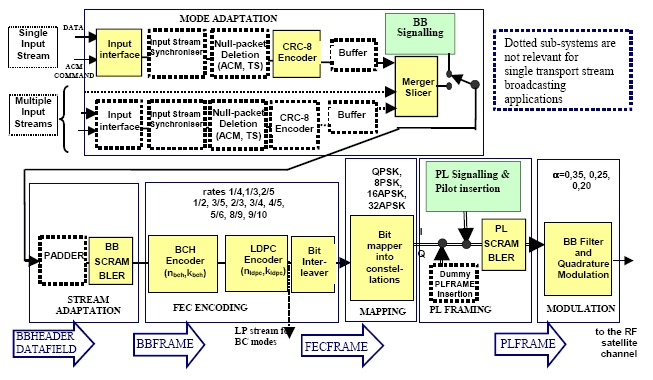
\includegraphics[scale=0.6]{DVBS2}
\caption{Functional block diagram of DVB-S2 ACM modem architecture} \label{fig:DVBSys}
\end{figure}


\subsection{Sub-Blocks Description}

The following subsystems description is organized according to the functional block diagram in \figref{fig:DVBSys}.

\subsubsection{Mode Adaptation}

DVB-S2 modem architecture deals with various input sequences:
\begin{itemize}
\item Single or multiple Transport Streams (TS), which are characterized by User Packets (UPs) of constant length equal to \(\unit{UPL} = 188\unit{bytes}\) (one MPEG packet) whose first byte is a sync-byte (\(47\ped{HEX}\));
\item Single or multiple Generic Streams (GS), which are characterized by continuous bit streams or streams of constant length user packets.
\end{itemize}
The first input bit is interpreted as the most significant bit (MSB). ACM command signalling allows setting of the transmission parameters to be adopted by DVB-S2 modulator, for a specific portion of input data.

Since the DVB-S2 modulator may produce variable transmission delay on the user information, the Input Stream Synchronizer provides a means to guarantee a constant bit rate (CBR) and constant end-to-end transmission delay.

The identification and erasure of MPEG null-packets allow to reduce the information rate and increase the error protection in the modulator. This process is carried out in a way that the removed null-packets can be re-inserted in the receiver in the exact place where they originally were. Specifications on this process are available in dedicated annex in \cite{b:DVBstandard}.

A systematic Cyclic Redundancy Check (CRC) encoding is provided so that the receiver can detect the presence of errors in received streams. The CRC of 8 bits is inserted in the Base-Band Header (BBHEADER), which has the overall length of 80 bits. BBHEADERs contain also other signaling information such as indications on the roll-off factor of the shaping filter (Square Root Raised Cosine), the presence/absence of padding bits, Adaptive/Constant Coding Modulation, the use of identification and erasure of null-packet function, etc.

\subsubsection{Stream Adaptation}
Stream adaptation (see \figref{fig:strformat}) provides padding to complete a constant length (\(k\ped{bch}\) bits) BBFRAME. \(k\ped{bch}\) depends on the FEC rate, as reported in \tbref{tb:codpar}. Padding may be applied in circumstances when the user data available for transmission are not sufficient to completely fill a BBFRAME, or when an integer number of UPs has to be allocated in a BBFRAME.
The input stream consists of a BBHEADER followed by a DATA FIELD. The output stream will be a BBFRAME.
\begin{figure} \centering
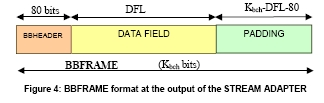
\includegraphics{data}
\caption{BBFRAME format at the output of the STREAM ADAPTER}\label{fig:strformat}
\end{figure}
\begin{description}
\item[PADDING] \(k\ped{bch} - \mathrm{DFL}-80\) zero bits are appended after the DATA FIELD so that the resulting BBFRAME have a constant length of \(k\ped{bch}\) bits. For Broadcast Service applications, \(\mathrm{DFL}= k\ped{bch}-80\), therefore no padding must be applied.
\item[SCRAMBLING] The complete BBFRAME should be randomized and the randomization sequence should be synchronous with the BBFRAME, starting from the MSB and ending after \(k\ped{bch}\) bits. Scrambling sequences are typically generated by feed-back shift registers. There are two main reasons why scrambling is used:
    \begin{itemize}
    \item It facilitates the work of a timing recovery circuit, an automatic gain control and other adaptive circuits of the receiver (eliminating long sequences consisting of 0 or 1 only).
    \item  It eliminates the dependence of a signal's power spectrum upon the actual transmitted data, making it more dispersed to meet maximum power spectral density requirements (because if the power is concentrated in a narrow frequency band, it can interfere\footnote{Standardization committees such as ETSI (European Telecommunications Standard Institute) have imposed various rules as to interferences.} with adjacent channels due to the cross modulation and the intermodulation caused by non-linearities of the receiving tract).
    \end{itemize}
\end{description}

\subsubsection{FEC Encoding}

This subsystem performs Outer Coding (BCH), Inner Coding (LDPC) and Bit Interleaving. The input stream is composed of BBFRAMEs and the output stream of FECFRAMEs.

Each BBFRAME (\(k\ped{bch}\) bits) is processed from the MSB to LSB by the FEC coding subsystem to generate a FECFRAME (\(n\ped{ldpc}\) bits). The parity check bits (BCHFEC) of the systematic BCH outer code must be appended after the BBFRAME and the parity check bits (LDPCFEC) of the inner LDPC encoder must be appended after the BCHFEC field, as shown in \figref{fig:fecformat}.

%We shall give more details as to FEC Encoding and Interleaving in the next sections.
\begin{figure} \centering
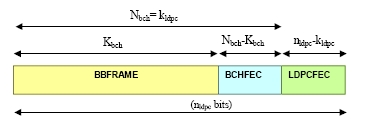
\includegraphics{FECformat}
\caption{Format of data before Bit Interleaving} \label{fig:fecformat}
\end{figure}

For 8PSK, 16APSK, and 32APSK modulation formats, the output of the LDPC encoder is bit interleaved using a block interleaver (see \figref{fig:BI} and \figref{fig:BI35}). Data is serially written into the interleaver column-wise, and serially read out row-wise (the MSB of BBHEADER is read out first, except 8PSK rate 3/5 case where MSB of BBHEADER is read out third) as shown in the figures.


\begin{figure} \centering
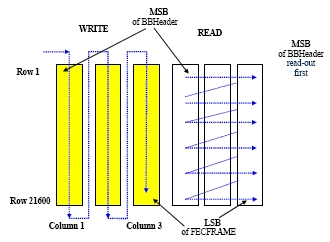
\includegraphics{Inter1}
\caption{Bit Interleaving scheme for 8PSK (for each rate except from 3/5) and normal FECFRAME length} \label{fig:BI}
\end{figure}


\begin{figure} \centering
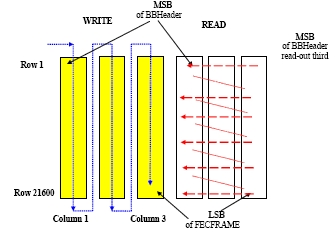
\includegraphics{Inter2}
\caption{Bit Interleaving scheme for 8PSK (rate 3/5) and normal FECFRAME length} \label{fig:BI35}
\end{figure}

\begin{table}
\begin{center}\begin{tabular}{|c|c|c|c|}
\hline
 Modulation &  Rows (\(n=64800\)) &  Rows (\(n=16200\)) & Columns \\
\hline
 8PSK &  21600 &  5400 & 3 \\
 16APSK &  16200 &  4050 & 4 \\
 32APSK &  12960 &  3240 & 5 \\
\hline
\end{tabular}\end{center}
\caption{Bit Interleaver structure}
\end{table}
%\section{Outer FEC: The BCH Code} \label{sec:BCHdes}

\subsubsection{Bit Mapping}

Each FECFRAME (which is a sequence of 64800 bits for normal FECFRAME, or 16200 bits for short FECFRAME), must be serial-to-parallel converted (parallelism level \(\eta\ped{MOD}\)= 2 for QPSK, 3 for 8PSK, 4 for 16APSK, 5 for 32APSK) in figures 9 to 12, the MSB of the FECFRAME is mapped into the MSB of the first parallel sequence.
Each parallel sequence shall be mapped into constellation, generating a \((I,Q)\) sequence of variable length depending on the selected modulation efficiency \(\eta\ped{MOD}\).

The input sequence is a FECFRAME, the output sequence is a XFECFRAME (compleX FECFRAME),
composed of \(\frac{64800}{\eta\ped{MOD}}\) (normal XFECFRAME) or \(\frac{16200}{\eta\ped{MOD}}\)
(short XFECFRAME) modulation symbols. Each modulation symbol is a complex vector in the format (I,Q) (I being the in-phase component and Q the quadrature
component) or in the equivalent format \( \rho \exp(\mathrm{j}\phi) \)(\(\rho\) being the modulus of the vector and \(\phi\) being its phase).


For QPSK, the System employs conventional Gray-coded QPSK modulation with absolute mapping (no differential coding). Bit mapping into the QPSK constellation is illustrated in \figref{fig:Q8PSK}. The normalized average energy per symbol is equal to \( \rho^2 = 1\).
Two FECFRAME bits are mapped to a QPSK symbol, i.e. bits \(2i\) and \(2i+1\) determines the \(i\)-th QPSK symbol, where \(i = 0 \virgola 1 \virgola 2 \virgola \ldots \virgola (N/2)-1\) and \(N \) is the coded LDPC block size.

For 8PSK, the System employs conventional Gray-coded 8PSK modulation with absolute mapping (no differential coding). Bit mapping into the 8PSK constellation is shown in \figref{fig:Q8PSK}. The normalized average energy per symbol is equal to \(\rho^2 = 1\).
For all the rates excluding \(3/5\), bits \(3i \virgola 3i+1 \virgola 3i+2 \) of the interleaver output determine the \(i\ap{th}\) 8PSK symbol where \(i = 0 \virgola 1 \virgola 2 \virgola \ldots \virgola (N/3)-1 \)and \(N\) is the coded LDPC block size. For rate 3/5 bits \(3i+2 \virgola 3i+1 \virgola 3i \) of the interleaver output determine the \(i\)-th 8PSK symbol where \(I = 0 \virgola 1 \virgola 2 \virgola \ldots \virgola (N/3)-1\) and \(N\) is the coded LDPC block size.

The 16APSK modulation constellation (see figure \figref{fig:Q8PSK}) is composed of two concentric rings of uniformly spaced 4 and 12 PSK points, respectively in the inner ring of radius \(\rho_1\) and outer ring of radius \(\rho_2\).
The ratio of the outer circle radius to the inner circle radius (\(\gamma =\rho_2/\rho_1\)) should be comply with \tbref{tb:16APSK_Radius}.
If \(4{\rho_1}^2+ 12{\rho_2}^2 = 16\) the average signal energy becomes 1.
Bits \(4i, 4i+1, 4i+2\) and \(4i+3\) of the interleaver output determine the \(i\)-th 16APSK symbol, where \(i = 0\virgola 1\virgola 2\virgola \ldots \virgola (N/4)-1\)
and \(N\) is the coded LDPC block size.

The 32APSK modulation constellation (see \figref{fig:Q8PSK}) is composed of three concentric rings of uniformly spaced 4, 12 and 16 PSK points, respectively in the inner ring of radius \(\rho_1\), the intermediate ring of radius \(\rho_2\) and the outer ring
or radius \(\rho_3\). \tbref{tb:32APSK_Radius} defines the values of \(\gamma_1 = \rho_2/\rho_1\) and \(\gamma_2 = \rho_3/ \rho_1\).
If \(4{\rho_1}^2+ 12{\rho_2}^2+ 16{\rho_3}^2 = 32\) the average signal energy becomes equal to 1.
Bits \(5i \virgola 5i+1 \virgola 5i+2 \virgola 5i+3\) and \(5i+4\) of the interleaver output determine the \(i\)-th 32APSK symbol, where \(i = 0 \virgola 1 \virgola 2 \virgola (N/5)-1\).

\begin{table}
\begin{center}\begin{tabular}{|c|p{1.47cm}||p{1.41cm}||p{1.56cm}||}
\hline
 Code Rate &  \multicolumn{1}{p{1.47cm}|}{\centering \(\eta\)} &  \multicolumn{1}{p{1.41cm}|}{\centering \(\gamma_1\)} &  \multicolumn{1}{p{1.56cm}|}{\centering \(\gamma_2\)} \\
\hline
 3/4 &  \multicolumn{1}{p{1.47cm}|}{\centering 3,74} &  \multicolumn{1}{p{1.41cm}|}{\centering 2,84} &  \multicolumn{1}{p{1.56cm}|}{\centering 5,27} \\
 4/5 &  \multicolumn{1}{p{1.47cm}|}{\centering 3,99} &  \multicolumn{1}{p{1.41cm}|}{\centering 2,72} &  \multicolumn{1}{p{1.56cm}|}{\centering 4,87} \\
 5/6 &  \multicolumn{1}{p{1.47cm}|}{\centering 4,15} &  \multicolumn{1}{p{1.41cm}|}{\centering 2,64} &  \multicolumn{1}{p{1.56cm}|}{\centering 4,64} \\
 8/9 &  \multicolumn{1}{p{1.47cm}|}{\centering 4,43} &  \multicolumn{1}{p{1.41cm}|}{\centering 2,54} &  \multicolumn{1}{p{1.56cm}|}{\centering 4,33} \\
 9/10 &  \multicolumn{1}{p{1.47cm}|}{\centering 4,49} &  \multicolumn{1}{p{1.41cm}|}{\centering 2,53} &  \multicolumn{1}{p{1.56cm}|}{\centering 4,3} \\
\hline
\end{tabular}\end{center}
\caption{Optimum constellation radius ratios \(\gamma_1\) and \(\gamma_2\) (linear channel) for 32APSK}
\label{tb:32APSK_Radius}
\end{table}
\begin{table}
\begin{center}\begin{tabular}{|c|c|c|}
\hline
 Code Rate &  \(\eta\) & \(\gamma\) \\
\hline
 2/3 &  2,66 & 3,15 \\
 3/4 &  2,99 & 2,85 \\
 4/5 &  3,19 & 2,75 \\
 5/6 &  3,32 & 2,7 \\
 8/9 &  3,55 & 2,6 \\
 9/10 &  3,59 & 2,57 \\
\hline
\end{tabular}\end{center}
\caption{Optimum constellation radius ratio \(\gamma\) (linear channel) for 16APSK} \label{tb:16APSK_Radius}
\end{table}

\subsubsection{Physical Layer (PL) Framing}
This block generates, synchronously with FECFRAMEs, physical layer frames (PLFRAMEs) and deal with
\begin{itemize}
\item the insertion of physical headers and optional pilot symbols (their insertion causes a loss of 2,4\% of capacity);
\item the insertion of dummy frames to be used in absence of data ready to be immediately transmitted;
\item the scrambling (or the randomization) for energy dispersal by multiplying the \((I+\im Q)\) samples by a complex radomization sequence \((C\ped{I}+ \im C\ped{Q})\).
\end{itemize}

\section{Inner and Outer FEC}

The DVB-S2 FEC section relies on two block codes concatenation, i.e., codewords generated by BCH encoder are, in turn, encoded by LDPC encoder\footnote{Note that each frame (either short or long) is processed from most significant to least significant bit, either by BCH or LDPC.}. Thus, BCH code is usually called \emph{outer code} and LDPC \emph{inner code}. Outputs from FEC encoding section are formatted according to \figref{fig:fecformat}. As we shall see later on, this BCH concatenation gives an extra protection \cite{b:DVBstandard} against unwanted error floors at high SNR\footnote{The \emph{iterative decoding} achieves very close to Shannon limit performance at low/medium  SNR. On the contrary, its performance may be significantly worse at high SNR. In fact, their free distance (the minimum Hamming distance between different codewords, i.e., the minimum Hamming weight of a nonzero codeword) can be low. This causes BER curve to flatten following the error floor tied to \(d\ped{free}\), after the waterfall region at low SNR. Performance of any binary code at high SNR can be well approximated by the expression of union bound, truncated to the contribution of free distance (terms at higher distance are negligible at high SNR). Such expression \cite{b:ErrFloor} is
\[
\mathrm{BER} \simeq \frac{1}{2}\frac{w\ped{free}}{k} \mathrm{erfc} \left( \sqrt{d\ped{free} \frac{k}{n}\frac{E\ped b}{N\ped 0} }\right)
\]}
When the decoding has to be performed, the above sequence of encoding steps must be, of course, inverted: in other words, LDPC starts to decode prior to BCH. As just said, error floor phenomena at high signal-to-noise ratio typically affect the decoding performance, and therefore the BCH extra protection against residual errors is aimed at counteracting to the performance degradation, enhancing FEC robustness at higher SNR.

In a some sense, the chain constituted, in order, by LDPC encoder, channel and LDPC decoder can be conceived as a super-channel on which BCH encoder/decoder operates. This kind of intuitive representation puts in evidence the advantage of concatenating two codes. The best choices on their kind of concatenation can give a powerful tool to enhance the performance of the overall FEC decoding, allowing to act by a outer coding on the weaknesses of the inner coding.


%\subsection{BCH design}
\subsection{BCH} \label{sec:BCHstruct}
BCH code is named for Bose, Ray-Chaudhury, and Hocquenghem, who published work in 1959 and1960 which revealed a means of designing codes over $GF(2)$ with a specified design distance. BCH codes are cyclic codes and thus, as explained in Appendix~B, can be specified by a generator polynomial.
In present Section we give only some notations over the particular, as we shall see, structure of BCH code employed in DVB-S2 and, more generally, over its design steps.

A BCH code of length $n$ with a specified minimum distance, or, i.e., capable of correcting (at least) $t$ errors, can be designed as follows \cite{b:moon,b:mcwilliams}:
\begin{enumerate}
\item Determine the smallest $m$ such that $GF(q^m)$ has primitive $n$th root (\secref{sec:factoring}) of unity $\beta$.
\item Select a nonnegative integer $b$. In most of cases, it is selected $b=1$.
\item Write down a list of $2t$ consecutive powers of $\beta$ (see \secref{sec:MathSurvey}):
\[
\beta^b \virgola \beta^{b+1} \virgola \ldots \virgola \beta^{b+2t-1}
\]
Determine the minimal polynomial of each of these powers of $\beta$. (Because of conjugacy, frequently these minimal polynomials are not distinct.)
\item The generator polynomial $g(x)$ is least common multiple (LCM) of these minimal polynomials. The code is a $(n\virgola n-\mathrm{deg}(g(x)))$ cyclic code.
\end{enumerate}

Two fields are involved in the construction of the BCH codes. The small field $GF(q)$ is where the generator polynomial has its coefficients and is the field where the elements of the codeword are. The big field $GF(q^m)$ is the field where the generator polynomial has its roots. For encoding purposes it is only sufficient to have the polynomial generator of the code, whereas, for decoding, the additionally knowledge of the extension field where the generator has its roots is necessary. Two definitions will be useful later on: first, if \(\beta\) selected is a primitive element then the code is called \emph{primitive}; second, when \(\beta=1\) the code is said to be a code in \emph{narrow-sense}.

It can be proved that following the constructive procedure described above produces codes with at least the specified minimum distance. As shown in Appendix B, since every codeword is a multiple of the generator polynomial, we can express the \emph{parity check condition} as follows
\begin{equation}
c(\beta^i)=m(\beta^i)g(\beta^i)=m(\beta^i)\cdot 0
\end{equation}
for \(i=b \virgola b+1 \virgola \ldots \virgola b+2t-1 \). In fact these powers of \(\beta\) are, by design, the roots of \(g(x)\). Rewriting these condition using the correspondent vector representation we get the following system of equations
\begin{equation}
c_0+c_1\beta^i+c_2\beta^{i+1}+\ldots+c_{n-1}{(\beta^{i})}^{n-1}=0
\end{equation}
always for \(i=b \virgola b+1 \virgola \ldots \virgola b+2t-1 \). Therefore \(2t\) parity check conditions can be also expressed in the matrix form
\begin{equation} \label{eq:pchk}
\left(
\begin{array}{ccccc}
  1 & \beta^i & \beta^{2i} & \cdots & \beta^{(n-1)i}
\end{array} \right)
\left(
\begin{array}{c}
  c_0 \\
  c_1 \\
  c_2 \\
  \vdots \\
  c_{n-1}
\end{array}
\right)
=0
\end{equation}
Stacking the row vectors for different values of \(i\) we get the following parity check matrix
\begin{equation}
\left(
  \begin{array}{ccccc}
    1 & \beta^b & \beta^{2b} & \ldots & \beta^{(n-1)b} \\
    1 & \beta^{b+1} & \beta^{2(b+1)} & \ldots & \beta^{(n-1)(b+1)} \\
    \vdots &  &  &  &  \\
    1 & \beta^{b+\delta-3} & \beta^{2(b+\delta-3)} & \ldots & \beta^{(n-1)(b+\delta-3)} \\
    1 & \beta^{b+\delta-2} & \beta^{2(b+\delta-2)} & \ldots & \beta^{(n-1)(b+\delta-2)} \\
  \end{array}
\right)
\end{equation}
where \(\delta=2t+1\) represent the \emph{design distance} (Hamming metric) of the code.

It can be proved (see \cite{b:moon}) that the matrix \(\vet H\) have at least \(\delta = 2t+1\) columns linearly dependent and, thus, the minimum distance of the code satisfies \( d\ped{min} \geq \delta \); that is, the code is capable of correcting at least \(t\) errors.

%\subsection{The Code Structure}

In DVB-S2 context, BCH outer code has been designed to avoid ``unpredictable and unwanted error floors which affect iterative decodings at high \(C/N\) ratios'', i.e., at low bit error rates (BER).

Although the mathematical background shown in this thesis in order to design, encoding and decoding is completely general, in the most practical cases the base fields of BCH codes is \(GF(2)\), as in DVB-S2 FEC section.  The polynomials which must be multiplied in order to obtain the wanted BCH code associated to a specific operating mode (or, i.e., error correction capability) are shown in Table \ref{tb:BCHpoly}. More specifically, multiplication of the first \(t\) of them provides a polynomial generator of the BCH code capable of correcting at least \(t\) error.   Notice that this procedure is in accordance with the third step to construct generator polynomial of the BCH code.

The encoding suggestions, provided in \cite{b:DVBstandard}, are typical of a cyclic codes in systematic form, whose specific properties and encoding steps are discussed in dedicated Appendix B. It is worth understanding that both systematic and non-systematic codewords are always multiple of the generator polynomial of the code (or, i.e., of the ideal, as also shown in \secref{sec:ideals}) so that parity check condition (\ref{eq:pchk}) is still valid as well as BCH bound. Furthermore, from a direct analysis of the polynomial supplied by \cite{b:DVBstandard} (Normal FEC-Frame), one could observe that these specific codes (one for each selected error protection level) are \emph{primitive} and, indeed, \emph{narrow-sense}. The reasons are described in the following

\begin{itemize}
\item \(g_1(x)\) is one of the possible primitive polynomial which has its roots in \(GF(2^{16})\). This can be quickly proved verifying that \(\alpha^{2^{16}-1}=1\) by computer aid or, more lazily, by direct consultation of any table of primitive polynomials. For the tables of primitive polynomials, the interested reader could refer to \cite{b:wicker}
\item Hence, this BCH is a narrow-sense code. In fact, by design, it follows that \(b\) must be equal to 1.
\end{itemize}

%Recalling that DVB-S2 transmission section operates in Adaptive Coding Modulation (ACM) we have -- always in Normal FEC-Frame mode -- different code rates to deal with variable link conditions.
Three different t-error correcting BCH codes (\(t=12\), \(t = 10\), \(t=8\)) should be applied to each BBFRAME, according to LDPC coding rates as shown in \tbref{tb:codpar}.
Outer FEC (i.e. BCH), although there are 11 LDPC coding rates, deal with only three different error protection level: \(t=12 \virgola t=10 \virgola t=8\). On the one hand we have, since this BCH is primitive, that the codeword length must be equal to \(2^{16}-1\). On the other hand we have in Table \ref{tb:codpar} multiple codeword lengths for each t-BCH code and all of them do not correspond to the primitive length BCH should have. %These questions raise an important point, especially in light of the above consideration as to the provided operating modes.
In general, for each code rate, a different set of polynomials to be multiplied would be expected, whereas, in DVB-S2, there is only one set of polynomials provided by \cite{b:DVBstandard}.

Eventually, we have to conclude that DVB-S2 BCH code is \emph{shortened}. A systematic \((n\virgola k)\) code can be shortened by setting a number of the information bits to zero (i.e, zero padding). This means that a linear \((n\virgola k)\) code consisting of $k$ information bits and \(n-k\) check bits (or redundancy bits) can be shortened into a \( (n-l \virgola k-l) \) linear code by setting the most (or the least, depending on the reference direction) significant first \(l\) bits to zero. As also described in \cite{b:moon}, shortening of a code does not have bad effects on its minimum distance properties and its decoding algorithms. However, shortened cyclic code might loose its cyclic property.



\begin{table} \centering
\begin{tabular}{|c|l|}
  \hline
  % after \\: \hline or \cline{col1-col2} \cline{col3-col4} ...
  \(g_1(x)\) & $1+x^2+x^3+x^5+x^{16}$ \\
  \(g_2(x)\) & $1+x+x^4+x^5+x^6+x^8+x^{16}$ \\
  \(g_3(x)\) & $1+x^2+x^3+x^4+x^5+x^7+x^8+x^9+ x^{10}+x^{11}+x^{16}$ \\
  \(g_4(x)\) & $1+x^2+x^4+x^6+x^9+x^{11}+ x^{12}+x^{14}+x^{16}$\\
  \(g_5(x)\) & $1+x+x^2+x^3+x^5+x^{8}+ x^{9}+x^{10}+x^{11}+x^{12}+x^{16}$ \\
  \(g_6(x)\) & $1+x^2+x^4+x^5+x^7+x^{8}+ x^{9}+x^{10}+x^{12}+x^{13}+x^{14}+x^{15}+x^{16}$\\
  \(g_7(x)\) & $1+x^2+x^5+x^6+x^8+x^{9}+ x^{10}+x^{11}+x^{13}+x^{15}+x^{16}$ \\
  \(g_8(x)\) & $1+x+x^2+x^5+x^6+x^{8}+ x^{9}+x^{12}+x^{13}+x^{14}+x^{16}$ \\
  \(g_9(x)\) & $1+x^5+x^{7}+ x^{9}+x^{10}+x^{11}+x^{16}$ \\
  \(g_{10}(x)\) & $1+x+x^2+x^5+x^7+x^{8}+ x^{10}+x^{12}+x^{13}+x^{14}+x^{16}$ \\
  \(g_{11}(x)\) & $1+x+x^2+x^3+x^5+x^{9}+ x^{11}+x^{12}+x^{13}+x^{16}$ \\
  \(g_{12}(x)\) & $1+x+x^5+x^6+x^{7}+ x^{9}+x^{11}+x^{12}+x^{16}$ \\
  \hline
\end{tabular}
\caption{BCH minimal polynomials for normal FECFRAME \(n\ped{LDPC}=64800\)}
\label{tb:BCHpoly}
\end{table}

\begin{table} \centering
\begin{tabular}{|c|c|c|c|c|}
  \hline
  LDPC Code  & BCH Uncoded & BCH Coded  & BCHFEC & BCH t-error\\
  Rate & Block & Block & & Correction\\
  \hline
  % after \\: \hline or \cline{col1-col2} \cline{col3-col4} ...
  1/4 & 16008 & 16200 & 192 & 12 \\
  1/3 & 21408 & 21600 & 192 & 12 \\
  2/5 & 25728 & 25920 & 192 & 12 \\
  1/2 & 32208 & 32400 & 192 & 12 \\
  3/5 & 38688 & 38880 & 192 & 12 \\
  2/3 & 43040 & 43200 & 160 & 10 \\
  3/4 & 48408 & 48600 & 192 & 12 \\
  4/5 & 51648 & 51840 & 192 & 12 \\
  5/6 & 53840 & 54000 & 160 & 10 \\
  8/9 & 57472 & 57600 & 128 & 8 \\
  9/10 & 58192 & 58320 & 128 & 8 \\
  \hline
\end{tabular}
\caption{Coding parameters for normal FECFRAME \(n\ped{LDPC}=64800\)} \label{tb:codpar}
\end{table}

\subsection{LDPC}

%\section{Inner FEC: Low Density Parity Check Code}

LDPC codes \cite{b:LDPCGall} were invented in 1960 by R. Gallager. They were largely ignored until the discovery of turbo codes \cite{b:Turbo} in 1993. Since then, LDPC codes have experienced a renaissance and are now one of the most intensely studied areas in coding.
%In this article we review the basic structure of LDPC codes and the iterative algorithms that are used to decode them. We also briefly consider the state of the art of LDPC design.

%In the year 1993, C. Berrou, A. Glavieux, and P. Thitimajshima presented their
%approach to error correcting coding, termed turbo coding, to the world. The new technique, with complexity only a small factor larger than that of standard coding schemes like convolutional codes, enables performance approaching the Shannon capacity of the additive white Gaussian noise channel within a fraction of a dB.
%
%In 1960 R. Gallager completed his Ph.D. thesis, Low-Density Parity-Check Codes.
%In this remarkable thesis Gallager introduced at least two lasting concepts: a powerful bounding technique to assess the maximum-likelihood performance of coding systems, and low-density parity-check (LDPC) codes together with their associated iterative decoding algorithm.


Much of the effort in coding over the last 50 years has focused on the construction of highly structured codes with large minimum distance. The structure keeps the decoding complexity manageable, while large minimum distance is supposed to guarantee good performance. This approach, however, is not without its drawbacks.
First, it seems that finding structured codes with large minimum distance turn out to be a harder problem than researchers imagined. Finding good codes in general is, in a sense, trivial: randomly chosen codes are good with high probability. More generally, one can easily construct good codes provided one admits sufficient \emph{description complexity} into the definition of the code. This conflicts, however, with the goal of finding
highly structured codes that have simple decodings.
Second, close to capacity, minimum distance is only a poor surrogate for the performance measure of real interest. Iterative coding systems take an entirely different approach. The basic idea is the following. Codes are constructed so that the relationship between their bits (the structure of their redundancy) is \emph{locally} simple, admitting simple
\emph{local decoding}.
The local descriptions of the codes are interconnected in a complex (e.g., random-
like) manner, introducing long-range relationships between the bits. Relatively high global description complexity is thereby introduced in the interconnection between the simple local structures. Iterative decoding proceeds by performing the simple local decodings and then exchanging the results, passing messages between locales across the `complex' interconnection. The locales repeat their simple decodings, taking into account the new information provided to them from other locales. Usually, one uses a graph to
represent this process. \emph{Locales} are nodes in the graph, and interconnections are represented as edges. Thus, description complexity is introduced without adding computational complexity per se, but rather as wiring or routing complexity.

In addition to the classical representation of block codes (i.e. by \(\vet H\) matrix), another useful and common way of representing an LDPC codes is through a graphical representation called a \emph{Tanner graph} \cite{b:LDPCGall, b:moon, b:MacKay}.
Tanner graphs of LDPC codes are bipartite graphs with variable nodes on one side and constraint nodes on the other. Each variable node corresponds to a bit, and each constraint node corresponds to one parity-check constraint on the bits defining a codeword. A parity-check constraint applies to a certain subset of the codeword bits, those that participate in the constraint. The parity-check is satisfied if the XOR of the participating bits is 0 or, equivalently, the modulo 2 sum of the participating bits is 0. Edges in the graph attach variable nodes to constraint nodes indicating that the bit associated with the variable node participates in the parity-check constraint associated with the constraint node. A bit sequence associated with the variable nodes is a codeword if and only if all of the parity-checks are satisfied.

\begin{figure}\centering
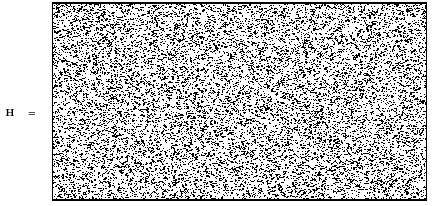
\includegraphics[scale=0.8]{sparseH}
\caption{A low-density parity-check matrix with \(N = 20000\) columns of weight \(j = 3\) and \(M = 10000\) rows of weight \(k = 6\) (reference \cite{b:MacKay}).} \label{fig:sparseH}
\end{figure}

The Tanner graph representation of the LDPC code closely mirrors the more standard
parity-check matrix representation of a code. In this latter description the code is represented as the set of all binary solutions \( \vet x = (x_1 \virgola x_2 \virgola \ldots \virgola x_n)\) to a simple linear algebraic equation (parity check equations \cite{b:mcwilliams, b:wicker, b:moon, b:MacKay}) \( \vet H \vet x\ap{T} = \vet 0\ap{T}\).
The elements of the parity-check matrix are 0s and 1s, and all arithmetic is modulo 2, that is, multiplication of \(\vet x\) by a row of \(\vet H\) means taking the XOR of the bits in \(\vet x\) corresponding to the 1s in the row of \(\vet H\). The connection between the parity-check matrix representation and the Tanner graph is straightforward, and is illustrated in \figref{fig:Tanner} by means of an example.
The elements of \(\vet x\) are in one-to-one correspondence with the variable
nodes in the Tanner graph. Thus, the variable nodes correspond to the columns of \(\vet H\).
The parity checks on \(\vet x\) are in one-to-one correspondence with the constraint nodes in the Tanner graph. Thus, the constraint nodes corresponds to the rows of \(\vet H\). The edges in the Tanner graph correspond to the 1s in \(\vet H\), that is, the entry in the
\(i\)-th row and \(j\)-th column of \(\vet H\) is a 1 if and only if the \(i\)-th constraint node is connected to the \(j\)-th variable node in the Tanner graph.

The Tanner graph captures the dependency structure of the various bits.
The iterative decoding algorithms we will discuss work directly on this bipartite graph.
Iterative algorithms for LDPC codes are message-passing and flipping algorithms, both introduced by Gallager \cite{b:LDPCGall}.

\begin{figure}\centering
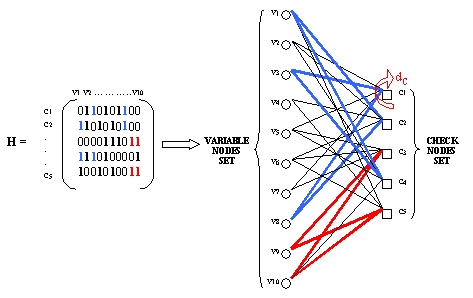
\includegraphics[scale=0.8]{LDPC}
\caption{A parity check matrix \(\vet H\) and the corresponding Tanner graph. To illustrate the relationship more clearly, some edge are shown in red or blue.} \label{fig:Tanner}
\end{figure}

\subsubsection{Iterative Decodings and Message-Passing}
In \emph{message-passing} decoders, messages are exchanged along the edges of the graph, and computations are performed at the nodes, as shown in \figref{fig:Belief}. Each message represents an estimate of the bit associated with the edge carrying the message.
These decoders can be understood by focusing on one bit as follows. Suppose the bits of an LDPC codeword are transmitted over a communications channel and, during transmission, some of them are corrupted so that a 1 becomes a 0 or vice versa.
Each bit node in the decoder gets to see the bit that arrived at the receiver corresponding to the one that was transmitted from the equivalent node at the
transmitter. Imagine that the node would like to know if that bit is in error or not and therefore asks all of its neighboring check nodes what they think the bit�s value should be. Each neighboring check node then asks their other neighbors what their bit values are and sends back to the original bit node the modulo 2 sum of those values.
The bit node now has several opinions as to the bit�s correct value and must somehow reconcile these opinions; it could, for example, take a majority vote. The above procedure constitutes one round or iteration of message passing.

\begin{figure}\centering
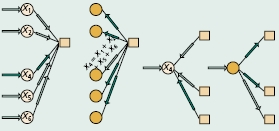
\includegraphics[scale=0.8]{beliefprop}
\caption{The principle of a message-passing decoder. Messages represent an
estimate of the bit associated with the edge carrying the message. Nodes query
neighboring nodes to collect opinions, process this information, and forward
their current estimate to their neighbors.} \label{fig:Belief}
\end{figure}

In order to improve performance, a further
such round can be performed. In more detail,
assume that those bit nodes that send their
observed bits to the checks to be summed first
ask their check node neighbors what they think is
their correct bit value. Those check nodes could
then query their other variable node neighbors
and forwarded their modulo 2 sum as an opinion.
With more information now available, the bit
nodes would have a better chance of communicating
the correct value to the check nodes, and
the opinions returned to the original node would
therefore have a better chance of being correct.
This gathering of opinions could obviously be
extended through multiple iterations; typically,
many iteration rounds are performed.

In actual decoding all nodes decode concurrently.
Each node gathers opinions from all its
neighbors and forwards to each neighbor an
opinion formed by combining the opinions of
the other neighbors. This is the source of the
term message passing. The process continues
until either a set of bits is found that satisfies all
checks or time runs out. The message passing
may proceed asynchronously. Note that with
LDPC codes, convergence to a codeword is easy
to detect since one need only verify that the parity
checks are satisfied.

The processing required for message-passing decoding LDPC codes is highly parallelizable and flexible. Each message-passing operation performed at a node depends on other nodes only through the messages that arrive at that node.
Moreover, message updating need not be synchronized. Consequently, there is great freedom to distribute in time and space the computation required to decode LDPC codes. Turbo codes are also decoded using belief propagation, but their structure does not admit the same level of atomization.

%In the above example, opinions about a bit
%were expressed as a binary value for that bit.
%Much better decoding is possible if the opinions
%are expressed as probabilities. If the transmitted
%bits are received in error with probability p, the
%probability that the observed bit is correct is 1 � p.
%If a check node forms a modulo 2 sum of k of
%these bits, the probability that the sum is correct is
%(1+(1 � 2p)k)/2. Thus, the opinions returned from
%the check nodes have a different probability of
%being correct than those coming from the channel.
%If the bit nodes properly take these probabilities
%into account when combining the opinions, better
%performance results. In the belief propagation algorithm
%the nodes assume that all incoming probabilities
%are independent and then combine them
%by applying the rules of probability.

There is a second distinct class of decoding algorithms
that is often of interest for very high speed
applications, such as optical networking.
This class of algorithms is known as flipping
algorithms. Bit flipping usually operates on
hard decisions: the information exchanged
between neighboring nodes in each iteration is a
single bit.
The basic idea of flipping is that each
bit, corresponding to a variable node assumes a
value, either 0 or 1, and, at certain times, decides
whether to flip itself (i.e., change its value from
a 1 to a 0 or vice versa). That decision depends
on the state of the neighboring check nodes
under the current values. If enough of the neighboring
checks are unsatisfied, the bit is flipped.
The notion of `enough' may be time-varying,
and it may also depend on soft information
available about the bit. Thus, under flipping,
variable nodes inform their neighboring check
nodes of their current value, and the check
nodes then return to their neighbors the parity
of their values. The underlying assumption is
that bits that are wrong will tend to have more
unsatisfied neighbors than bits that are correct.


%LDPC codes are linear binary block codes. The codewords can be expressed as the set of all binary solutions \((x_1 \virgola x_2 \virgola \ldots \virgola x_n)\) to the parity check equation
%\(\vet H \vet x\ap{T}= 0\), where the parity check matrix \(\vet H\) is a binary matrix. The codeword length is represented by \(n\). Each row of H induces one parity check
%constraint on x. The number of independent constraints is n-k, and k is the
%number of information bits that can be encoded with this code.
%Low-Density Parity-Check (LDPC) codes are called low-density because they
%are defined by giving a parity-check matrix H that is sparse, i.e., it has few
%nonzero entries.
%
%Another useful and common way of representing an LDPC codes is through a
%graphical representation called a Tanner graph, see Fig. 1. A Tanner graph of
%an LDPC code is a bipartite graph with variable nodes on one side and
%constraint or check nodes on the other side. Variable nodes correspond one-to-
%one with bits xi, hence they correspond to the columns of H. Constraint
%nodes correspond one-to-one with the parity checks that the bits xi must
%satisfy, hence they correspond to the rows of H. Edges in the graph connect
%constraint nodes to variable nodes, where an edge indicates the associated bit
%participates in the associated parity check. Thus, the edges in the graph
%correspond to the 1�s in the parity-check matrix H. A bit sequence associated
%to the variable nodes is a codeword if and only if the modulo 2 sum of the bits
%that neighbor a check node is 0 for all check nodes.



%Turbo codes have very close to Shannon limit performance at low/medium  SNR. On the contrary, turbo codes performance may be significantly worse at high SNR. In fact, their free distance (the minimum Hamming distance between different codewords, i.e., the minimum Hamming weight of a nonzero codeword) can be low. This causes BER curve to flatten following the error floor tied to \(d\ped{free}\), after the waterfall region at low SNR (typically at error rates major than \(10^{-6}\)).
%More specifically, performance of any binary code at high SNR can be well approximated by the expression of union bound, truncated to the contribution of free distance (terms at higher distance are negligible at high SNR). A small penalty deriving from sub-optimality (iterative decoding only approximates a ML decision) of iterative decoding should be taken into the account. As a consequence, we have
%\begin{equation}
%BER \simeq \frac{1}{2}\frac{w\ped{free}}{k} \mathrm{erfc} \left( \sqrt{d\ped{free} \frac{k}{n}\frac{E\ped b}{N\ped 0} }\right)
%\end{equation}

\subsubsection{Encoding Procedure for The DVB-S2 Code}

The LDPC code of DVB-S2 standard has the following structure (see the Annex A in \cite{b:DVBstandardTR})

\begin{equation}
\vet H = \left[
\begin{array}{c|c}
\vet H\ap{d} & \vet H\ap{p}
\end{array} \right]
\end{equation}
where \(\vet H\ap{d}\) is an \(r \times k\) matrix, and \(\vet H\ap{p}\) is a dual diagonal \(r \times r\) matrix that is shown below for example (\(r=5\))

\begin{equation}
\vet H\ap{p} = \left(
\begin{array}{ccccc}
1 & 0 & 0 & 0 & 0\\
1 & 1 & 0 & 0 & 0\\
0 & 1 & 1 & 0 & 0\\
0 & 0 & 1 & 1 & 0\\
0 & 0 & 0 & 1 & 1
\end{array} \right)
\end{equation}
The notation in use is the same employed as far in standard description, that is, \(r= n-k\) represents the number of redundancy bits, \(n\) the codeword length, and \(k\) the length of messages to be encoded. By now, it does not matter which rate LDPC has: clearly \(\vet H\) size change with coding rates and so its composition.

Codewords, represented by vector \(\vet x\), can be divided in a systematic part, namely \(\vet  s\), and a part relevant to the redundancy (parity) bits, namely \(\vet p\), in a way such that vector \(\vet x\) can be expressed as \(\vet x=(\vet s\virgola \vet p)\ap{T}\). The encoding is accomplished by searching the parity vector \(\vet p\) which satisfies the (system) equation \(\vet {Hx}= \vet 0\). This system, as the \(\vet x\), can be divided in two contributes as follows
\begin{equation}
\vet H\ap{d} \vet s + \vet H\ap{p} \vet p= \vet 0 \text{     or     } \vet H\ap{d} \vet s =\vet H\ap{p} \vet p= \vet v
\end{equation}
which is obviously equivalent to that given before.

So the encoding process can be carried out through two steps:
\begin{enumerate}
\item Determine the auxiliary vector \(\vet v=\vet{H}\ap{d}\vet s\). The number of XOR operations to do is \((n-k)\cdot(d\ped{c}-1)\), where \(d\ped{c}\) is the number of 1s in a row of \(\vet H\ap{d}\), which is constant in a regular LDPC.
\item Determine the \(r\) parity bits by a back substitution, using the equation \(\vet H\ap{p}\vet p = \vet v\), i.e.,
\begin{equation}
\begin{align}
p_1 &= v_1 \\
p_l &= v_l + p_{l-1}  & \text{for } l= 1 \virgola 2 \virgola \ldots\virgola r
\end{align}
\end{equation}
Here the number of operations (XOR) required is \(r-1\). This is actually a matrix inversion process, which can be almost costless executed because the matrix is bi-diagonal.
\end{enumerate}
The encoder structure is shown in \figref{fig:LDPCENC}. The overall number of operations to be performed is \(n(1-R)(d\ped{c}-1)\) (\(R\), as usually indicated in the vast majority of literature, is the code rate) and thus the encoder complexity grows linearly with \(n\).

\begin{figure}\centering
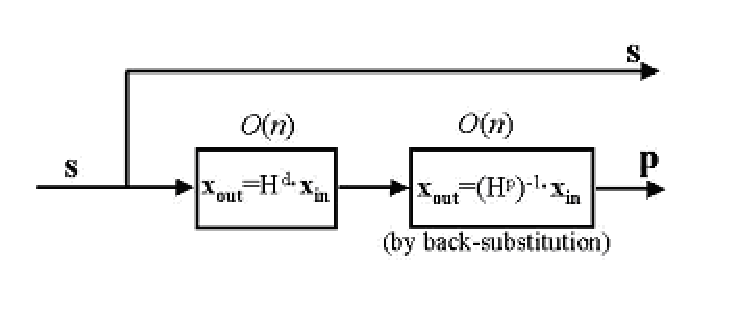
\includegraphics[scale=0.8]{LDPCENC}
\caption{Encoding process of random-like LDPC codes} \label{fig:LDPCENC}
\end{figure}

The very regular structure of \(\vet H\) matrix allows to minimize the amount of memory to be allocated so as to succeed in storing the position of one in there even when using the brute force to do that. However, the full matrix, during the encoding, is recovered from compressed information, which is contained in dedicated tables for each, of course, coding rate provided.

For example, only the location of the ones in the first column of \(\vet H\ap{d}\) is described by the table (in the first table row) in the standard: the following 359 columns are obtained through a cyclic shift of the first column of a number of locations starting from the first column.
In the same way, only the location of the ones in the 361st column of H is described by the table (second table row) in the standard: the following 359 columns are obtained via a cyclic shift of a number of locations starting from the 361st column. This procedure is followed up to the last (\(k\)-th) column of \(\vet H\ap{d}\).

Let us now recall the procedure indicated by ETSI in \cite{b:DVBstandard}.
The DVB-S2 LDPC encoder systematically encodes an information block of size \(k\ped{ldpc}\), \(\vet i= (i_0\virgola i_1\virgola i_2\virgola \ldots \virgola i_{k\ped{ldpc}})\) onto a codeword of size \(n\ped{ldpc}\), \(\vet c=(i_0\virgola i_1 \virgola \ldots \virgola p_0\virgola p_1 \virgola \ldots \virgola p_{n\ped{ldpc}-k\ped{ldpc}-1})\). The transmission of codewords starts in the given order from \(i_0\) and ends with \(p_{n\ped{ldpc}-k\ped{ldpc}-1}\). LDPC code parameters \((n\ped{ldpc}\virgola k\ped{ldpc})\) are given in table    These last two parameters depend on the coding rate and the code block size, which may be either normal or short.

The procedure to calculate the parity bits for each kind of block is the following
\begin{itemize}
\item Set all the parity bits to zero, that is, \(p_0=p_1=\ldots=p_{n\ped{ldpc}-k\ped{ldpc}-1}=0\)
\item Accumulate the first information bit, namely \(i_0\), at the parity address specified in the fist row of Tables B1 through B8 in Annex B \cite{b:DVBstandard}. %For example, for a 2/3 rate, we obtain
\item The structure of \(\vet H\) matrix can be now exploited in this way: the second column, indicating over which element of the output the second information bit is accumulated, can be obtained by the first column, and so on for the other columns. Hence
    \begin{itemize}
    \item For the next 359 information bits accumulate \(i_m\) at parity bit addresses \( \left\{ x + (r \mod 360\times q)\right\} \mod (n\ped{ldpc}-k\ped{ldpc}) \) where \(x\) denotes the address of the parity bit accumulator corresponding to the first bit \(i_0\), and \(q\) is a code rate dependent constant specified in Table 7a in \cite{b:DVBstandard}.
    \item For the 361th information bit \(i\ped{360}\), the addresses of parity bit accumulators are given in the second row of the tables B1 through B8 in Annex B \cite{b:DVBstandard}. In a similar way the addresses of the parity bit accumulators for the following 359 information bits, namely \(i_m \virgola i=361\virgola 362 \virgola \ldots \virgola 719\), are obtained using the formula \( \left\{ x + (r \mod 360\times q)\right\} \mod (n\ped{ldpc}-k\ped{ldpc}) \) where \(x\) denotes the address of the parity bit accumulator corresponding to the information bit \(i_{360}\), i.e., the entries in the second row of the tables B1 through B8 in Annex B \cite{b:DVBstandard}.
    \end{itemize}
\item In a similar manner, for every group of 360 new information bits, a new row from tables B1 through B8 in Annex B \cite{b:DVBstandard} are used to find the addresses of the parity bit accumulators.

\end{itemize}

After all of the information bits are exhausted, the final parity bits are obtained as follows (this is back substitution introduced before, now executed in-place, i.e., with no use of auxiliary vector):
\begin{itemize}
\item Sequentially perform the following operations starting with \(i=1\)
\begin{equation}
p_i = p_i + p_{i-1}\virgola \text{          } i= 0 \virgola 1 \virgola \ldots\virgola n\ped{ldpc}-k\ped{ldpc}-1
\end{equation}
\item Final content of \(p_i \virgola i= 0 \virgola 1 \virgola \ldots\virgola n\ped{ldpc}-k\ped{ldpc}-1\) is equal to the parity bit \(p_i\).
\end{itemize}

Following considerations can be done:
\begin{enumerate}
\item 	The sparse matrix \(\vet H\ap d\) is constituted by \(N\ped{S}\) sub-matrices (number of rows of tables B1 through B8) with \(r\)-rows and 360-columns, each of which is specified by a row of the tables B1 through B8; in detail, addresses of ones in the first column of each matrices is specified by a row of these tables.
\item 	Each column of  the sub-matrices constituting \(\vet H\ap d\) can be obtained via a cyclic shift of the first column,  in which the shift is of a number of positions (rows) equal to \(q\). The shift is cyclic since it is reduced modulo \(m\), the number of the rows of each sub-matrix.
\item	\(\vet H\ap d\)  has a fixed number of ones per row (\(d\ped c\)), depending on coding rate.
\item 	Number of ones per column in each sub-matrix is not fixed; tables B1 through B8 in fact has \textbf{col1} columns in the first \textbf{row1} rows and \textbf{col2} columns for \textbf{row2} (=\(N\ped{S}\)-row1) rows; this means that first \textbf{row1} sub-matrices of \(\vet H\ap d\) have \textbf{col1} ones per column, while \textbf{row2} sub-matrices have \textbf{col2} ones per column.
\item \(\vet H\ap p\) is a \(r \times r\) bi-diagonal matrix.
\end{enumerate}

\begin{figure}\centering
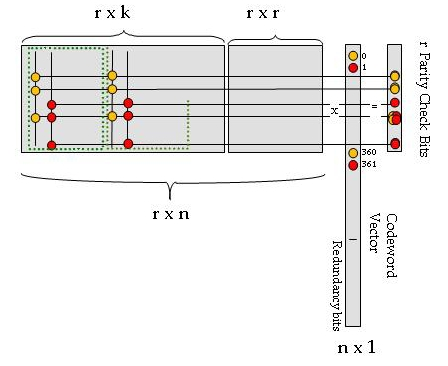
\includegraphics[scale=0.8]{LDPCProd}
\caption{Regularity properties of the LDPC generation matrix} \label{fig:LDPCProd}
\end{figure}


The code rate dependant constant \(q\) (introduced in paragraph before) allows a division of total number \(r\) of check equations in q congruence classes; each of them has 360 equations (\(r=360\cdot q\)). From this point of view and considering tables associated to LDPC coding procedure, a parity check equation can be identified by a couple of parameters \(R\) and \(Q\): the congruence class (\(R_x\)) and the position (\(Q_x\)) in the congruence class. These parameters are obtained from following relations:
\begin{subequations}
\begin{align}
R_x &= B_x \mod q \\
Q_x &= \frac{B_x}{q}
\end{align}
\end{subequations}
where \(B_x\) is a generic element of address tables B1 trough B8, \(0<R<q-1\) and \(0<Q<359\). These tables are used to address systematic bits to the corresponding check equation.

All parameters of the encoding procedure are summarized in \tbref{tb:LDPCENCPAR}, where in order from left to right we have:
\begin{enumerate}
\item Rate: LDPC coding rate
\item \(r=n-k\): number of code parity bits
\item \(q = 180\cdot (1-R)\): code rate dependent constant
\item \(d\ped{c}\): check nodes degree (number of bits per parity check equation)
\item \(N\ped{S}=180-q=k/360= \vet{row1}+\vet{row2}\): number of sub-matrices \(r\times 360\) of \(\vet H\ap{NS}\)
\item \textbf{row1}: number of sub-matrices with \textbf{col1} ones per column
\item \textbf{row2}: number of sub-matrices with \textbf{col2} ones per column
\item \textbf{col1}: variable nodes degree with \(0<index<360\cdot \vet{row1}\)
\item \textbf{col2}: variable nodes degree with \(360\cdot \vet{row1}<index< k\)
\item \#Bx: total number of elements in tables B1 through B8
\end{enumerate}

\begin{table}
\begin{center}\begin{tabular}{|c|cccccccccc|}
\hline
 Rate &  \(d\ped{c}\) &  \(q\) &  \(N\ped{S}\) &  \(k\) bit &  \(r\) bit &  \textbf{row1} &  \textbf{row2} &  \textbf{col1} &  \textbf{col2} & \#Bx \\
\hline
 1/4 &  2 &  135 &  45 &  16200 &  48600 &  15 &  30 &  12 &  3 & 270 \\
 1/3 &  3 &  120 &  60 &  21600 &  43200 &  20 &  40 &  12 &  3 & 360 \\
 2/5 &  4 &  108 &  72 &  25920 &  38880 &  24 &  48 &  12 &  3 & 432 \\
 1/2 &  5 &  90 &  90 &  32400 &  32400 &  36 &  54 &  8 &  3 & 450 \\
 3/5 &  9 &  72 &  108 &  38880 &  25920 &  36 &  72 &  12 &  3 & 648 \\
 2/3 &  8 &  60 &  120 &  43200 &  21600 &  12 &  108 &  13 &  3 & 480 \\
 3/4 &  12 &  45 &  135 &  48600 &  16200 &  15 &  120 &  12 &  3 & 540 \\
 4/5 &  16 &  36 &  144 &  51840 &  12960 &  18 &  126 &  11 &  3 & 576 \\
 5/6 &  20 &  30 &  150 &  54000 &  10800 &  15 &  135 &  13 &  3 & 600 \\
 8/9 &  25 &  20 &  160 &  57600 &  7200 &  20 &  140 &  4 &  3 & 500 \\
 9/10 &  28 &  18 &  162 &  58320 &  6480 &  18 &  144 &  4 &  3 & 504 \\
\hline
\end{tabular}\end{center}
\caption{LDPC parameters for the encoding procedure. }\label{tb:LDPCENCPAR}
\end{table}

\section{Modem Performance} \label{sec:Perf}

Spectral efficiency provided by DVB-S2 ranges from about \(0,5 \unit{bps {Hz}^{-1}}\), using the QPSK \(1/4\), to \(4,5 \unit{bps {Hz}^{-1}}\), using the 32APSK \(9/10\); \(E\ped{s}/N\ped 0\) goes from \(-2,4 \unit{dB}\) to \(16\unit{dB}\) (AWGN channel and an ideal demodulation have been assumed), as also illustrated in \figref{f:Perf2}. This performance has been computed by computer simulations \cite{b:DVBS2system, b:DVBstandardTR} at a Packet Error Rate (PER) equal to \(10^{-7}\), corresponding about to one erroneous Transport Stream Packet per transmission hour in a \(5 \unit{Mbit/s}\) video service
On an AWGN channel\footnote{We remind that the performance over AWGN channels represents in communications an upper bound to the performance over more realistic channels. For this reason, comparison of the performance between two systems can be accomplished without any loss of generality over an AWGN environment. Comparisons under gaussian hypotheses are expected to be virtually the same over any non-gaussian environment/channel.}, DVB-S2 gives an increase of transmission capacity (about 20-35\%) compared to DVB-S and DVB-DNSG under the same transmission conditions.

The DVB-S2 system may be used in `single carrier per transponder' or in `multiple-carriers per transponders' (FDM). On a transponder with the single carrier configuration, the transmission rate \(R\ped{s}\) can be adapted to available bandwidth (at \(-3\unit{dB}\)) in order to obtain the maximum transmission capacity compatible with the acceptable signal degradation due to transponder bandwidth limitations. In the multiple-carrier configuration (Frequency Division Multiplexing), the symbol rate \(R_s\) must be adapted to the BS (Broadcasting Services) frequencies interval so as to optimize transmissive capacity while keeping the mutual interferences between adjacent carriers at acceptable level.

\figref{f:Perf} shows the performance achieved by the modem architecture with respect to the unconstrained (from modulation levels and block length of codes) Shannon limit. The ideal \(\frac{E\ped b}{N\ped 0}\) ratios in \tbref{tb:EtaPerf} for each operating mode has been derived from the ideal \(\frac{E\ped s}{N\ped 0}\) ratios by using the following dB-relation \begin{equation}
\frac{E\ped b}{N\ped 0} = \frac{E\ped s}{N\ped 0} - 10\log_{10}(\eta\ped{CM})
\end{equation}
where \(\eta\ped{CM}\) is the ideal joint efficiency of modulation and coding adopted to transmit symbols.

\figref{f:Perf2} shows, over the plane \(C/N\) -- spectral efficiency, the overall performance compared to either the constrained Shannon bounds or the DVB-S performance.
The gain of DVB-S2 with respect to DVB-S in terms of \(C/N\), for a given spectral efficiency, remains virtually constant, around \(2-2,5 \unit{dB}\) \cite{b:DVBstandardTR, b:DVBstandard}.


\begin{figure} \centering
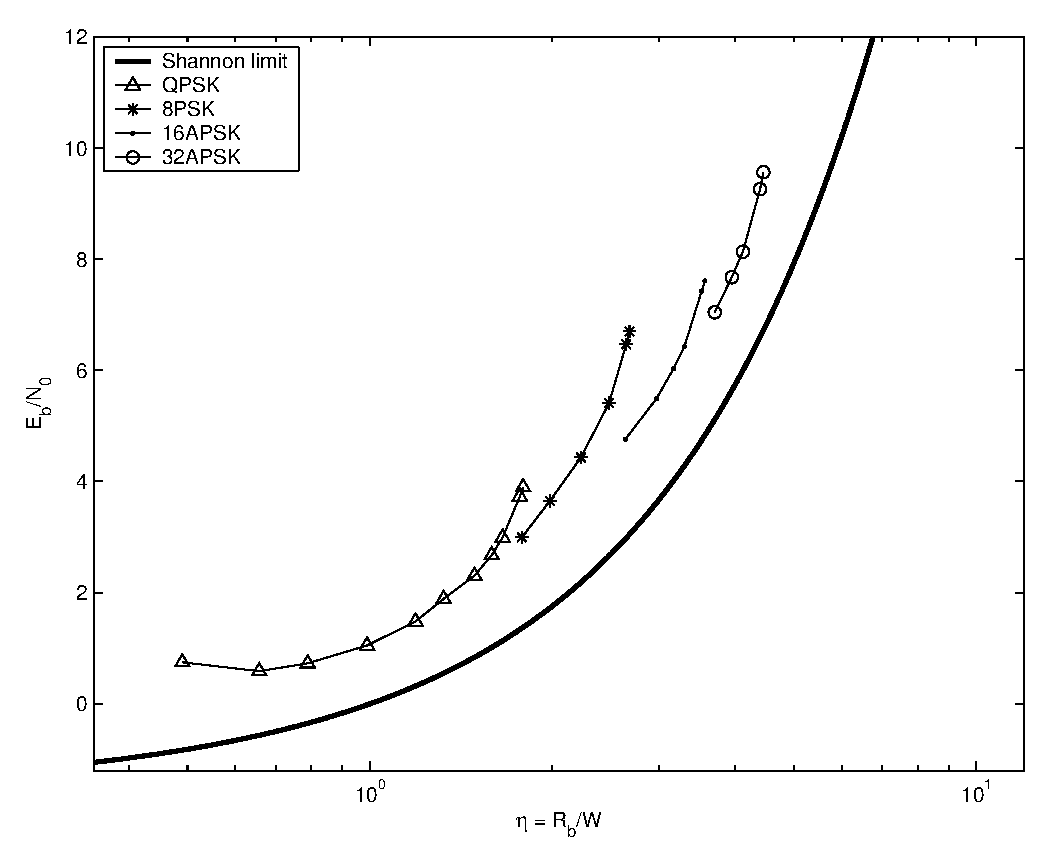
\includegraphics[scale = 0.3]{performance}
\caption{Performance of DVB-S2 for each modulation format and coding rate at \(\mathrm{PER}=10^{-7}\) with respect to absolute Shannon limit}\label{f:Perf}
\end{figure}

\begin{figure} \centering
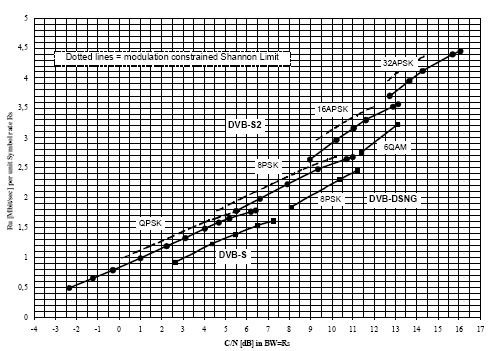
\includegraphics[scale = 0.7]{PvsShConstr}
\caption{Performance Shannon limits constrained} \label{f:Perf2}
\end{figure}

\begin{table}
\begin{center}\begin{tabular}{|c|p{1.88cm}||p{2.47cm}||p{2.78cm}||p{2.84cm}||}
\hline
 Modulation &  \multicolumn{1}{p{1.88cm}|}{\centering Coding rate (LDPC)} &  \multicolumn{1}{p{2.47cm}|}{\centering Spectral efficiency} &  \multicolumn{1}{p{2.78cm}|}{\centering Ideal \(E\ped{s}/N\ped 0\) for normal FECFRAME} &  \multicolumn{1}{p{2.84cm}|}{\centering Ideal \(E\ped b/ N\ped 0\) for normal FECFRAME} \\
\hline
 QPSK &  \multicolumn{1}{p{1.88cm}|}{\centering 1/4} &  \multicolumn{1}{p{2.47cm}|}{\centering 0,490243} &  \multicolumn{1}{p{2.78cm}|}{\centering -2,35} &  \multicolumn{1}{p{2.84cm}|}{\centering 0,75} \\
 QPSK &  \multicolumn{1}{p{1.88cm}|}{\centering 1/3} &  \multicolumn{1}{p{2.47cm}|}{\centering 0,656448} &  \multicolumn{1}{p{2.78cm}|}{\centering -1,24} &  \multicolumn{1}{p{2.84cm}|}{\centering 0,59} \\
 QPSK &  \multicolumn{1}{p{1.88cm}|}{\centering 2/5} &  \multicolumn{1}{p{2.47cm}|}{\centering 0,789412} &  \multicolumn{1}{p{2.78cm}|}{\centering -0,3} &  \multicolumn{1}{p{2.84cm}|}{\centering 0,73} \\
 QPSK &  \multicolumn{1}{p{1.88cm}|}{\centering 1/2} &  \multicolumn{1}{p{2.47cm}|}{\centering 0,988858} &  \multicolumn{1}{p{2.78cm}|}{\centering 1} &  \multicolumn{1}{p{2.84cm}|}{\centering 1,05} \\
 QPSK &  \multicolumn{1}{p{1.88cm}|}{\centering 3/5} &  \multicolumn{1}{p{2.47cm}|}{\centering 1,188304} &  \multicolumn{1}{p{2.78cm}|}{\centering 2,23} &  \multicolumn{1}{p{2.84cm}|}{\centering 1,48} \\
 QPSK &  \multicolumn{1}{p{1.88cm}|}{\centering 2/3} &  \multicolumn{1}{p{2.47cm}|}{\centering 1,322253} &  \multicolumn{1}{p{2.78cm}|}{\centering 3,1} &  \multicolumn{1}{p{2.84cm}|}{\centering 1,89} \\
 QPSK &  \multicolumn{1}{p{1.88cm}|}{\centering 3/4} &  \multicolumn{1}{p{2.47cm}|}{\centering 1,487473} &  \multicolumn{1}{p{2.78cm}|}{\centering 4,03} &  \multicolumn{1}{p{2.84cm}|}{\centering 2,31} \\
 QPSK &  \multicolumn{1}{p{1.88cm}|}{\centering 4/5} &  \multicolumn{1}{p{2.47cm}|}{\centering 1,587196} &  \multicolumn{1}{p{2.78cm}|}{\centering 4,68} &  \multicolumn{1}{p{2.84cm}|}{\centering 2,67} \\
 QPSK &  \multicolumn{1}{p{1.88cm}|}{\centering 5/6} &  \multicolumn{1}{p{2.47cm}|}{\centering 1,654663} &  \multicolumn{1}{p{2.78cm}|}{\centering 5,18} &  \multicolumn{1}{p{2.84cm}|}{\centering 2,99} \\
 QPSK &  \multicolumn{1}{p{1.88cm}|}{\centering 8/9} &  \multicolumn{1}{p{2.47cm}|}{\centering 1,766451} &  \multicolumn{1}{p{2.78cm}|}{\centering 6,2} &  \multicolumn{1}{p{2.84cm}|}{\centering 3,73} \\
 QPSK &  \multicolumn{1}{p{1.88cm}|}{\centering 9/10} &  \multicolumn{1}{p{2.47cm}|}{\centering 1,788612} &  \multicolumn{1}{p{2.78cm}|}{\centering 6,42} &  \multicolumn{1}{p{2.84cm}|}{\centering 3,89} \\
 8PSK &  \multicolumn{1}{p{1.88cm}|}{\centering 3/5} &  \multicolumn{1}{p{2.47cm}|}{\centering 1,779991} &  \multicolumn{1}{p{2.78cm}|}{\centering 5,5} &  \multicolumn{1}{p{2.84cm}|}{\centering 3,00} \\
 8PSK &  \multicolumn{1}{p{1.88cm}|}{\centering 2/3} &  \multicolumn{1}{p{2.47cm}|}{\centering 1,980636} &  \multicolumn{1}{p{2.78cm}|}{\centering 6,62} &  \multicolumn{1}{p{2.84cm}|}{\centering 3,65} \\
 8PSK &  \multicolumn{1}{p{1.88cm}|}{\centering 3/4} &  \multicolumn{1}{p{2.47cm}|}{\centering 2,228124} &  \multicolumn{1}{p{2.78cm}|}{\centering 7,91} &  \multicolumn{1}{p{2.84cm}|}{\centering 4,43} \\
 8PSK &  \multicolumn{1}{p{1.88cm}|}{\centering 5/6} &  \multicolumn{1}{p{2.47cm}|}{\centering 2,478562} &  \multicolumn{1}{p{2.78cm}|}{\centering 9,35} &  \multicolumn{1}{p{2.84cm}|}{\centering 5,41} \\
 8PSK &  \multicolumn{1}{p{1.88cm}|}{\centering 8/9} &  \multicolumn{1}{p{2.47cm}|}{\centering 2,646012} &  \multicolumn{1}{p{2.78cm}|}{\centering 10,69} &  \multicolumn{1}{p{2.84cm}|}{\centering 6,46} \\
 8PSK &  \multicolumn{1}{p{1.88cm}|}{\centering 9/10} &  \multicolumn{1}{p{2.47cm}|}{\centering 2,679207} &  \multicolumn{1}{p{2.78cm}|}{\centering 10,98} &  \multicolumn{1}{p{2.84cm}|}{\centering 6,70} \\
 16APSK &  \multicolumn{1}{p{1.88cm}|}{\centering 2/3} &  \multicolumn{1}{p{2.47cm}|}{\centering 2,637201} &  \multicolumn{1}{p{2.78cm}|}{\centering 8,97} &  \multicolumn{1}{p{2.84cm}|}{\centering 4,76} \\
 16APSK &  \multicolumn{1}{p{1.88cm}|}{\centering 3/4} &  \multicolumn{1}{p{2.47cm}|}{\centering 2,966728} &  \multicolumn{1}{p{2.78cm}|}{\centering 10,21} &  \multicolumn{1}{p{2.84cm}|}{\centering 5,49} \\
 16APSK &  \multicolumn{1}{p{1.88cm}|}{\centering 4/5} &  \multicolumn{1}{p{2.47cm}|}{\centering 3,165623} &  \multicolumn{1}{p{2.78cm}|}{\centering 11,03} &  \multicolumn{1}{p{2.84cm}|}{\centering 6,03} \\
 16APSK &  \multicolumn{1}{p{1.88cm}|}{\centering 5/6} &  \multicolumn{1}{p{2.47cm}|}{\centering 3,300184} &  \multicolumn{1}{p{2.78cm}|}{\centering 11,61} &  \multicolumn{1}{p{2.84cm}|}{\centering 6,42} \\
 16APSK &  \multicolumn{1}{p{1.88cm}|}{\centering 8/9} &  \multicolumn{1}{p{2.47cm}|}{\centering 3,523143} &  \multicolumn{1}{p{2.78cm}|}{\centering 12,89} &  \multicolumn{1}{p{2.84cm}|}{\centering 7,42} \\
 16APSK &  \multicolumn{1}{p{1.88cm}|}{\centering 9/10} &  \multicolumn{1}{p{2.47cm}|}{\centering 3,567342} &  \multicolumn{1}{p{2.78cm}|}{\centering 13,13} &  \multicolumn{1}{p{2.84cm}|}{\centering 7,61} \\
 32APSK &  \multicolumn{1}{p{1.88cm}|}{\centering 3/4} &  \multicolumn{1}{p{2.47cm}|}{\centering 3,703295} &  \multicolumn{1}{p{2.78cm}|}{\centering 12,73} &  \multicolumn{1}{p{2.84cm}|}{\centering 7,04} \\
 32APSK &  \multicolumn{1}{p{1.88cm}|}{\centering 4/5} &  \multicolumn{1}{p{2.47cm}|}{\centering 3,951571} &  \multicolumn{1}{p{2.78cm}|}{\centering 13,64} &  \multicolumn{1}{p{2.84cm}|}{\centering 7,67} \\
 32APSK &  \multicolumn{1}{p{1.88cm}|}{\centering 5/6} &  \multicolumn{1}{p{2.47cm}|}{\centering 4,11954} &  \multicolumn{1}{p{2.78cm}|}{\centering 14,28} &  \multicolumn{1}{p{2.84cm}|}{\centering 8,13} \\
 32APSK &  \multicolumn{1}{p{1.88cm}|}{\centering 8/9} &  \multicolumn{1}{p{2.47cm}|}{\centering 4,397854} &  \multicolumn{1}{p{2.78cm}|}{\centering 15,69} &  \multicolumn{1}{p{2.84cm}|}{\centering 9,26} \\
 32APSK &  \multicolumn{1}{p{1.88cm}|}{\centering 9/10} &  \multicolumn{1}{p{2.47cm}|}{\centering 4,453027} &  \multicolumn{1}{p{2.78cm}|}{\centering 16,05} &  \multicolumn{1}{p{2.84cm}|}{\centering 9,56} \\
\hline
\end{tabular}\end{center}
\caption{DVB-S2 performance at \(\unit{PER}=10^{-7}\)}\label{tb:EtaPerf}
\end{table} 


\chapter{BCH Encoding Algorithms for DVB-S2 Digital Transmissions} \label{ch:BCHAlg&Arch}


\section{Encoding Algorithm Description}

As introduced in Section , the systematic encoding of a message
\begin{equation}
 \vet m = (m_{k\ped{BCH}-1} \virgola m_{k\ped{BCH}-2} \virgola \ldots  \virgola m_{1} \virgola m_{0})
\end{equation}
here expressed in vectorial form, provides a codeword
\begin{equation}
\vet c = (m_{k\ped{BCH}-1} \virgola m_{k\ped{BCH}-2} \virgola \ldots  \virgola m_{1} \virgola m_{0} \virgola d_{n\ped{BCH}-k\ped{BCH}-1} \virgola \ldots \virgola d_0)
\end{equation} \label{eq:codsyst}
composed of \(r=n\ped{BCH}-k\ped{BCH}\) redundancy bits, aimed at protecting information messages, in the least significant positions. Codewords in systematic form have in the most significant positions the exact replica of information bits.

According to the cyclic code theory (see Appendix B), the systematic encoding of messages can be carried out through these three steps:
\begin{enumerate}
\item Multiplication of the message polynomial $m(x)$ by $x^r$. It can be easily realized through a left shift of the information bits by $r$ positions and a zero padding of the least significant $r$ bits.
\item Division of this vector by the polynomial generator. Coefficients of the remainder, expressed in polynomial form
    \begin{equation}
    d(x) = d_{r-1}x^{r-1} +  d_{r-2}x^{r-2} + \ldots+ d_1 x^1 + d_0 \label{eq:remainder}
    \end{equation}
    represent the \(r\) parity bits.
\item Finally, as also stated in \secref{sec:algebraicstruct},
\begin{equation} \label{eq:systematic}
 x^{r}m(x)-d(x)
\end{equation}
provides a codeword. Furthermore, since we are in $GF(2)$ and thus $-d(x) = d(x)$, the expression \eqref{eq:systematic} can be rewritten as
\begin{equation}
 x^{r}m(x)+d(x) \label{eq:sistematica}
\end{equation}
\end{enumerate}

A signal flow diagram of a possible polynomial division implementer is given in \figref{fig:PolyDiv}. This kind of architecture is usually called Linear Feedback Shift Register because of the feedback wire connecting the last stage with the first stage of the register. We shall show that the LSFR can succeed in computing the remainder (or parity) bits. This linear system provides instant-by-instant quotient and remainder bits together.

It is possible to demonstrate that this LFRS yields at each sampling instant the temporary remainder bits, which in turns have to be updated at the next time instant. Let us give an intuitive proof of this only focusing on the remainder bits (state) evolution of LFSR. Hereafter we will work only with polynomial coefficients in GF(2), even if generalizations in other base fields\footnote{Very synthetically, multiplier and adder in LFSR shown in \figref{fig:SerEnc} have to implement these operation in Galois arithmetic.} are straightforward (e.g. see \cite{b:mcwilliams, b:wicker, b:moon, b:ProakisDG}) .

The binary digits in register, after a certain number of computation cycles required (by now it does not matter how many cycles are required), represent the remainder of division. It is useful to observe that taking the remainder after division by \(g(z)=z^4+z^2+1\) is as imposing \(z^4=z^2+1\)\footnote{Over the real field, for example, taking the remainder after division by 4 of any number is as imposing \(4=0\) so that \(13 \textrm{mod} 4 = 1\) because 13 can be thought as \(4\times3+1\) and, given that \(4=0\), then the remainder is 1.}.
This operation is performed by the feedback and taps (i.e. those represented as \(g_1\virgola g_{r-1}\) in \figref{fig:PolyDiv}) of the LFSR.

Since degree of \(g(z)\) is 4, the shift register length must be 4 (the remainder of division is a polynomial of degree \(r=3\), which thus have 4 coefficients) as well as the second taps (i.e. \(g_2\)) must be enabled. If the message, from MSB to LSB, \(m(z)=z^8+z^4\) enters the first sum (modulo 2) node, we have a delay line between entering bit and bit in \(x_3\) equals to 4. This means that by the feedback wire and taps enabling/disabling all the polynomial coefficients are relatively summed with those of the same degree. When, for example, a \(z^8\) generates the partial result \(r(z)=(1+z^2)\) corresponding to \(z^4(1+z^2)\) at the fifth time instant, the entering coefficient is relevant to degree 4 and then must be summed with the one carried by the feedback wire in order to update \(x_0\).

Using the equivalent polynomial notation, let us describe the temporal sequence of all the operations performed.
\begin{enumerate}
\item All the register flip flops are set to 0. Coefficient of \(z^8\) enter \(x_0\), so determining \(\vet x =  (1\virgola0\virgola1\virgola0)\). We can represent the polynomial division together with digits in the flip flops by the following expression
    \[ (r_{1}(z)=1+0\cdot z^1+0\cdot z^2+0\cdot z^3)\cdot z^8\]
    where \(r_{i}(z)\) represent the partial remainder at \(i\)-th iteration.

\item \[(r_{2}(z)=0+1\cdot z^1+0\cdot z^2+0\cdot z^3)\cdot z^7 + (m_2(z) = 0\cdot z^7)\]
\item \[(r_{3}(z)=0+0\cdot z^1+1\cdot z^2+0\cdot z^3)\cdot z^6 + (m_3(z) = 0\cdot z^6)\]
\item \[(r_{4}(z)=0+0\cdot z^1+0\cdot z^2+1\cdot z^3)\cdot z^5 + (m_4(z) = 0\cdot z^5)\]
\item Here we have \((r_{5}(z)=1+0\cdot z^1+1\cdot z^2+0\cdot z^3)\cdot z^4 + (m_5(z) = 1\cdot z^4)\) and then
    \[
    (r_{5}(z)=0+0\cdot z^1+1\cdot z^2+0\cdot z^3)\cdot z^4
    \]
\item
\[(r_{6}(z)=0+0\cdot z^1+0\cdot z^2+1\cdot z^3)\cdot z^3 + (m_6(z) = 0\cdot z^3)\]
\item
\[(r_{7}(z)=1+0\cdot z^1+1\cdot z^2+0\cdot z^3)\cdot z^2+ (m_7(z) = 0\cdot z^2)\]
\item
\[(r_{8}(z)=0+1\cdot z^1+0\cdot z^2+1\cdot z^3)\cdot z^1+ (m_8(z) = 0\cdot z^1)\]
\item
\[(r_{9}(z)=1+0\cdot z^1+0\cdot z^2+0\cdot z^3)\cdot z^0+ (m_9(z) = 0\cdot z^0)\]
\(r(z)=r_9(z)\) corresponding to \(\vet x=(1\virgola0\virgola0\virgola0)\) is also the result of division by \(g(z)\).
\end{enumerate}
The key observation to be made in order to understand the encoding process is interpreting each delay tier as the degree of a polynomial (like \(z\)-transform).

For the architecture in \figref{fig:SerEnc}, analogous observations upon delay tier between input and output can be made. Here the entering coefficients are summed with the maximum degree coefficients of the partial remainder \(r_{i}(z)\) at each clock cycle, and thus the delay tier is exactly 0. If the result of this sum is 1 then the feedback is enabled, else it does not. As we shall show in the next section, the choice of feeding the shift register by the right-hand side allows us to achieve better performance.

\section{Serial Architectures} \label{sec:SArch}

A problem not yet dealt with is how (and when) the parity bits, once computed, can be extracted from the register. As shown in the previous section, LFSR in  \figref{fig:PolyDiv} gives the parity bits as all the bits of message-zero-padded, \(m(x)x^r\), enter the fist sum (modulo 2) node. Therefore, provided that the remainder after division can be fetched and stored in a single clock tick, this LFSR takes \(n\ped{BCH}\) clock cycles to yield the wanted result.

It is interesting to notice that only at a certain discrete time instant (they furthermore fall periodically) the registers of LFSR contain redundancy bits representing the remainder after division. This drawback prevents this type of architecture from working serially because results of division algorithm have to be properly fetched and stored in any other register when the parity bits are ready.

As just noticed, architecture in \figref{fig:PolyDiv} is slightly unsuitable for a serial systematic encoder since results of divisions (redundancy bits) have to be read in parallel at every \((j+1) n\ped{BCH}\) instant for \(j= 0 \virgola 1 \virgola 2 \ldots\). This can be technically performed, but however the architecture would not be serial anymore. Nevertheless, these facts will become quite interesting in parallelization of the architecture.

On the other hand, a mere serial hardware architecture is illustrated in Figure \ref{fig:SerEnc}. Differently from above, here the encoder is fed by the opposite side, thus immediately enabling the feedback, allowing the structure so devised to yield the remainder at every $(j+1) k\ped{BCH}$ instead of $(j+1) n\ped{BCH}$ for  \(j= 0 \virgola 1 \virgola 2 \ldots\). This permits to read serially parity bits and, besides, set (each register is reset) the device so as to make it ready to encode properly next incoming bit streams.
Serial encoding in systematic form is accomplished (see \figref{fig:SerEnc}) by:

\begin{description}
\item[ Systematic Bits Transmission and Parity Computation]
For clock cycles 1 to $k\ped{BCH}$, the information bits are transmitted in the natural order (switch S2 in position 2), while also feeding the shift register, to allow parity bits to be calculated in the Linear Feedback Shift Register (LFSR) (to that purpose, switch S1 must be on, activating the feedback mode).
\item[Parity Bits Transmission]
For clock cycles $k\ped{BCH}+1$ to $n\ped{BCH}$, the parity bits in the LFSR are transmitted (switch S2 in position 1) and the LFSR feedback mode is switched off (by setting S1 off).
\end{description}

From the above timing consideration, it follows that the latter architecture, spending \(k\ped{BCH}\) clock cycles against \(n\ped{BCH}\), performs more efficiently encoding in case of parallel fetching of the parity bits, as we shall see later on.
%In general, there are two ways to encode an information stream. One that enables to encode the messages at  \(n\ped{BCH}\) clock cycles -- supposing the parity bits are fetched in parallel, i.e., in one clock tick --, another one that, under the same hypothesis, yields the redundancy bits  at \(n\ped{BCH}\) clock cycles.

\begin{figure}
\begin{signalflow}[node distance=9mm, xscale=1.2]%
   % The \tikzgrid environment creates a fixed sized grid, where each
   % node in the grid is placed using the familiar array syntax.
   % The grid size is set using the node distance option.
   % Tip: Use the xscale and yscale options to get different spacing in the
   %      x and y directions.
  \tikzgrid{
      % building blocks
         &
      \node[coordinate]       (c1)  {}           &
             &
      \node[node]       (n1)  {}           &
             &
      \node[node]       (n2)  {}           & &
      \node[coordinate] (c2)  {}           &
      \node[coordinate] (c3)  {}           &
      \node[node] (n3)        {}           & &
      \node[coordinate] (c4)  {}
      \\ &
        & &
      \node[multiplier] (m1)  {$g_1$} & &
      \node[multiplier] (m2)  {$g_2$} & & & &
      \node[multiplier] (mn)  {$g_{r-1}$}
      \\
      \node[input]     (in) {$u(i)$}      &
      \node[adder]      (a1)  {}           &
      \node[delay]      (b1) {$x_0$}       &
      \node[adder]      (a2)  {}           &
      \node[delay]      (b2) {$x_1$}       &
      \node[adder]      (a3)  {}           &
      \node[delay]      (b3) {$x_2$}       &
      \node[coordinate] (c5) {}            &
      \node[coordinate] (c6) {}            &
      \node[adder] (a4)  {}                &
      \node[delay]      (br) {$x_{r-1}$}   &
      \node[coordinate] (cr)  {}           &
  }
  % signal paths
  % r is short hand notation for a real signal.
  % Use c to get a complex style signal
  \path[r>] (in)--(a1);
  \path[r>] (c1)--(a1);
  \path[r>] (a1)--(b1);
  \path[r]  (br)--(cr);
  \path[r]  (cr)--(c4);
  \path[r>] (c4)--(n3);
  \path[r>] (n3)--(mn);
  \path[r>] (n3)--(c3);
  \path[r.] (c3)--(c2);
  \path[r>] (n2)--(n1);
  \path[r]  (n1)--(c1);
  \path[r>] (b3)--(c5);
  \path[r.] (c5)--(c6);
  \path[r>] (c6)--(a4);
  \path[r>] (a4)--(br);
  \path[r>] (mn)--(a4);
  \path[r>] (c2)--(n2);
  \path[r>] (n2)--(m2);
  \path[r>] (n1)--(m1);
  \path[r>] (m1)--(a2);
  \path[r>] (m2)--(a3);
  \path[r>] (b1)--(a2);
  \path[r>] (a2)--(b2);
  \path[r>] (b2)--(a3);
  \path[r>] (a3)--(b3);
\end{signalflow}
\caption{Linear Feedback Shift Register architecture implementing the polynomial division in $n\ped{BCH}$ clock cycles}\label{fig:PolyDiv}
\end{figure}

\begin{figure}\centering
%
%% Serial Architecture (Type 2: serial fetching)
\begin{signalflow}[node distance=10mm]%
   % The \tikzgrid environment creates a fixed sized grid, where each
   % node in the grid is placed using the familiar array syntax.
   % The grid size is set using the node distance option.
   % Tip: Use the xscale and yscale options to get different spacing in the
   %      x and y directions.
  \tikzgrid{
      % building blocks
      \node[coordinate]       (c1)  {}           &&
      \node[node]       (n1)  {}           &&
      \node[node]       (n2)  {}           & &
      \node[coordinate] (c2)  {}           &
      \node[coordinate] (c3)  {}           &
      \node[node] (n3)        {}           & &
      \node[node] (n4) {}                  &
      \node[coordinate] (c4)  {}
      \\
        & &
      \node[multiplier] (m1)  {$g_1$} & &
      \node[multiplier] (m2)  {$g_2$} & & & &
      \node[multiplier] (mn)  {$g_{r-1}$}
      \\
      \node[coordinate]  (a1)                 &
      \node[delay]      (b1) {$x_0$}       &
      \node[adder]      (a2)  {}           &
      \node[delay]      (b2) {$x_1$}       &
      \node[adder]      (a3)  {}           &
      \node[delay]      (b3) {$x_2$}       &
      \node[coordinate] (c5) {}            &
      \node[coordinate] (c6) {}            &
      \node[adder] (a4)  {}                &
     \node[delay]      (br) {$x_{r-1}$}   &
     \node[node]        (ny) {}     &
      \node[adder]      (cr)  {}           &
      \\ &&&&&&&&&
      \node[input] (in) {$u(i)$}       & &
      \node[node]  (n9) {}
      \\ &&&&&&&&&&
      \node[node] (n10) {}
    }
  % signal paths
  % r is short hand notation for a real signal.
  % Use c to get a complex style signal
  \path[r>]  (in)--(n9);
  \path[r] (c1)--(a1);
  \path[r>] (a1)--(b1);
  \path[r]  (br)--(cr);
  \path[r]  (cr)--(c4);
  \path[r>] (c4)--(n3);
  \path[r>] (n3)--(mn);
  \path[r>] (n3)--(c3);
  \path[r.] (c3)--(c2);
  \path[r>] (n2)--(n1);
  \path[r]  (n1)--(c1);
  \path[r>] (b3)--(c5);
  \path[r.] (c5)--(c6);
  \path[r>] (c6)--(a4);
  \path[r>] (a4)--(br);
  \path[r>] (mn)--(a4);
  \path[r>] (c2)--(n2);
  \path[r>] (n2)--(m2);
  \path[r>] (n1)--(m1);
  \path[r>] (m1)--(a2);
  \path[r>] (m2)--(a3);
  \path[r>] (b1)--(a2);
  \path[r>] (a2)--(b2);
  \path[r>] (b2)--(a3);
  \path[r>] (a3)--(b3);
 % \path[r>] (br)--(n7);
%  \path[r>] (n7)--(cr);
\end{signalflow}

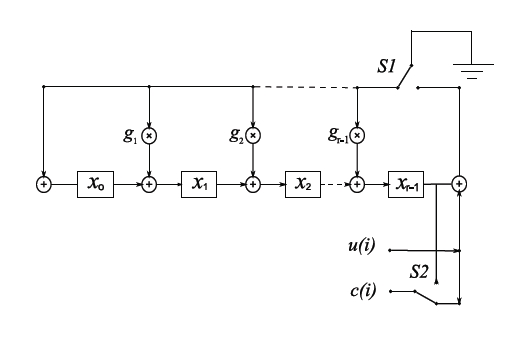
\includegraphics[scale=0.7]{serenc}
\caption{Serial encoder architecture based on LFSR (systematic encoding): it implements the systematic encoding of any codeword in \(n\ped{bch}\) clock ticks. At the end of each message encoding, encoder does not require a reset of the state register and thus is ready to immediately encode a new incoming message.} \label{fig:SerEnc}
\end{figure}
%\begin{figure}
%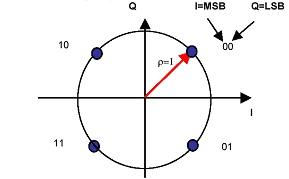
\includegraphics{4PSK}
%\caption{Serial encoder architecture implementing the polynomial division in $k\ped{BCH}$ clock cycles}\label{f:enck}
%\end{figure}

\section{Encoding Algorithms for Parallel Architectures}

\subsection{Modelling System} \label{s:model}

From the theory of control we know that any linear system, fed by an input signal \(\vet u(i)\) can be described by the following system of linear equation
\begin{subequations} \label{eq:LinSys}
\begin{align}
\vet y(i) & = \vet {Cx}(i) + \vet{Du}(i) \label{subeq:GeneralOutput} \\
\vet x(i+1) &= \vet {Ax}(i) + \vet{Bu}(i) \label{subeq:GeneralState}
\end{align}
\end{subequations}
where \eqref{subeq:GeneralOutput} expresses its outcomes \(\vet y(i)\) at each sampling (discrete) instant, while \eqref{subeq:GeneralState} describes its trajectory of state \(\vet x(i)\), i.e., the state evolution of the linear system in question. Without descending in further details, we shall particularize both equations for the linear feedback shift register shown in \figref{fig:PolyDiv} and, starting from them, find equations relevant to an architecture with a \(p\) degree of parallelism. We shall notice that they will perfectly match with system \eqref{eq:LinSys}.

The Linear Feedback Shift Register (LFSR) depicted in \figref{fig:PolyDiv} is a linear system, and thus can be described by the well known output equation expressing \( y(i)\), the scalar output, and the state transition equation expressing the vector state \(\vet x(i)\) as a function of the discrete time \(i\)
\begin{subequations} \label{eq:LFSR}
\begin{align}
 y(i) & = \vet {cx}(i) + d\cdot u(i) \\
\vet x(i+1) &= \vet {Ax}(i) + \vet{b}u(i) \label{eq:statequation}
\end{align}
\end{subequations}

In particular, for the desired parallel BCH encoding procedure, we are only interested in the (state) vector
\begin{equation}
\vet x(i) =
\left(
\begin{array}{ccccc}
  x_0(i)   & x_1(i) & \ldots  & \ldots & x_{r-1}(i) \\
\end{array}
\right)\ap T
\end{equation}
and in its temporal evolution/transition because \(\vet x(i)\) represents the parity bits after the required number of computation cycles. Thus, hereafter we shall focus only on \eqref{eq:statequation}. The scalar $u(i)$ indicates the input at the sampling instant $i$, as put in evidence in \figref{fig:PolyDiv} and \figref{fig:SerEnc}. The matrix \(\vet A\) models the state evolution of the system in absence of external stimulus (i.e., \(u(i)=0\)), and thus is usually called the state transition matrix. For analogous reasons, the column vector $\vet b$ is called as the input-to-state transfer relationship. %Let us recall that all the operations of this linear system has to be performed over $GF(2)$.

The form of \(\vet A \virgola \vet b\) depends uniquely on the position of taps and connections in the LFSR. In other words, that form is strongly dependent on the selected architecture implementing the encoding algorithm. More precisely, the matrix $\vet A$ depends on the taps collocations of LSFR, whereas vector $\vet b$ depends on where the input/s is/are connected to the system.

Now, referring to the LFSR architecture depicted in \figref{fig:PolyDiv}, which can yield the redundancy bits after $n\ped{BCH}$ clock cycles, we can write, on the one hand,
\begin{align}
\vet A & = \left (
\begin{array} {ccccc}
0      &  0     & \ldots &  0     & g_0\\
1      &  0     & \ldots & 0      & g_1\\
\vdots &  1     & \ldots &   0    & g_2\\
       & \vdots & \ldots & \vdots & \vdots\\
0      & 0      & \ldots & 1      & g_{r-1} \\
\end{array} \right ) &
\vet b & = \left(
\begin{array}{c}
  1 \\
  0 \\
   \vdots \\
    \vdots \\
    0\\
\end{array} \right) \label{eq:ParSyst}
\end{align}
where $\vet A$, $r$ by $r$ state transition square matrix, contains in the last column the polynomial generator coefficient except for its coefficient of maximum degree. On the other hand, column vector $\vet b$ of length $r$ gives a mathematical representation of the physical input-to-system connections.

As introduced in Section \ref{sec:SArch}, the adoption of the architecture in \figref{fig:SerEnc} permits to save some clock ticks. Not surprisingly, only $\vet b $ has changed its form whereas the representation of matrix $\vet A$ given in \eqref{eq:ParSyst} still holds. Since inputs enter now from the right-hand side, we have the new column vector
\begin{equation}\label{eq:vetb}
\vet b =
\left(
\begin{array}{c}
  g_0 \\
  g_1 \\
   \vdots \\
    \vdots \\
    g_{r-1}\\
\end{array}
\right)
\end{equation}
which models -- as before -- the input incidence on the system state.


\subsection{Parallel Linear System Description}

In the previous section we have briefly described a possible model of system
which can be easily exploited in parallelizing a general serial architecture
with a degree of parallelism $p$. Starting from \eqref{eq:statequation} and
applying instant-by-instant and recursively the following substitutions
\begin{align*}
\vet x(i) &= \vet {Ax}(i-1) + \vet{b}u(i-1)\\
\vet x(i-1) &= \vet {Ax}(i-2) + \vet{b}u(i-2)\\
\vdots \\
\vet x(i-p+1) &= \vet {Ax}(i-p) + \vet{b}u(i-p)\\
\vet x(i) &= \vet {A} \left[ \vet{Ax}(i-2) + \vet{b}u(i-2)\right] + \vet{b}u(i)\\
&= \vet A^2 \vet x (i-2) + \vet{Ab} u(i-2) + \vet{b} u(k-1)
\end{align*}
we can observe that the evolution of this system at a generic sampling instant $i$ depends on
\begin{itemize}
\item the state vector relevant to a generic former instant;
\item a set of former inputs whose cardinality is equal to the difference among the current time index and the former instant selected.
\end{itemize}

This is equivalent, from an architectural implementation point of view, in feeding the encoding processor by a set of parallel inputs, associating to each of the multiple input wires a different (multiple) time instant. Hence, parallelization is straightforwardly achieved.

Returning to the above expression, the system evolution for a generic degree of parallelism $p$ is modelled by the following state equation
\begin{equation}\label{eq:pseq}
\vet x(i) = \vet A^p(i-p) + \sum_{k=0}^{p-1}{\vet A^k \vet b u(i-k-1)}
\end{equation}
Now, setting the column vectors $\vet A^k \vet b$ as follows
\begin{equation}\label{eq:Bmatrix}
\left(
\begin{array}{ccccc}
  \vet b & \vet{Ab} & \ldots & \vet A^{p-2} \vet b &  \vet A^{p-1} \vet b
\end{array}
\right)
\end{equation}
we can define a new $r$ by $p$ $\vet B_p$ matrix which represent the incidence of the last $p$ inputs
\begin{equation}\label{eq:newu}
\vet u(ip) =
\left(
\begin{array}{ccccc}
  u(ip-1)   & u(ip-2) & \ldots  & \ldots & u \left[ p(i-1))\right] \\
\end{array}
\right)\ap T
\end{equation}
on the system evolution. Considering both \eqref{eq:Bmatrix} and \eqref{eq:newu}, we can therefore rewrite the state equation \eqref{eq:pseq} as
\begin{equation} \label{eq:SEmatr}
\vet x (ip) = \vet A^p \vet x \left[ (i-1)p \right] + \vet B_p \vet u(ip)
\end{equation}
where the sum $\sum_{k=0}^{p-1}{\vet A^k \vet b u(i-k-1)}$ has just been replaced by the above matrices product.

\subsection{Matrices Structure and Properties} \label{sec:Regularity}

In every practical case, the wanted degree of parallelism is strictly less than the number of registers containing the remainder bits at the end of every bit stream processing. For this reason, in this section we shall describe the main characteristics of matrices $\vet A^p$ and $\vet B_p$ only within the range $0 < p \le r$ of our interest.

Therefore for a generic degree $p$ (within the above specified range) we have
\begin{equation} \label{eq:Apreg}
\vet A^p =
\left(
\begin{array}{cc}
\vet 0 & \vet C_1 \\
\vet I & \vet C_2
\end{array}
\right)
\end{equation}
where
\begin{itemize}
\item \(\vet 0\) represents a null \(p \times p\) matrix;
\item $\vet I$ represent a square $r-p$ by $r-p$ identity matrix;
\item $\vet C_1$ is a $p \times p$ matrix where each row represents the combinatorial connections (1 when it is active, 0 otherwise) between last and first $p$ bits of vector $\vet x(i)$;
\item $\vet C_2$ is a $(r-p) \times p$ matrix where each row represents the combinatorial connections between last $p$ bits and the remaining bits of the vector \(\vet x(i)\)
\end{itemize}

Differently from $\vet A^p$ matrix, $\vet B_p$ as well as $\vet b$ (as just said in \secref{s:model}) is strictly dependent on where inputs are. Referencing to the LFSR architecture depicted in \figref{fig:PolyDiv}, we have therefore
\begin{equation} \label{eq:Btrivial}
\vet B_p =
\left(
\begin{array}{c}
\vet I \\
\vet 0
\end{array}
\right)
\end{equation}
in case on which the feedback starts at least (depends on the position of the first one in the message) after $\frac{r}{p}$ clock ticks (supposing that \(p\) is a divisor of \(r\)). Identity matrix has size $p\times p$. For example, for a \bch{7}{15} with a degree of parallelism $p=5$
\footnote{The degree of parallelism must be a divisor of numbers of clock ticks to encode a codeword. This architecture spends a number of ticks equal to 15 (codeword length) and therefore \(p\) can be 5.}
we get

\begin{align} \label{eq:triex}
\vet A^5 & =
\left( \begin{array}{cccccccc}
 0 &  0 &  0 &  1 &  1 &  0 &  1 & 0 \\
 0 &  0 &  0 &  0 &  1 &  1 &  0 & 1 \\
 0 &  0 &  0 &  0 &  0 &  1 &  1 & 0 \\
 0 &  0 &  0 &  0 &  0 &  0 &  1 & 1 \\
 0 &  0 &  0 &  1 &  1 &  0 &  1 & 1 \\
 1 &  0 &  0 &  0 &  1 &  1 &  0 & 1 \\
 0 &  1 &  0 &  1 &  1 &  1 &  0 & 0 \\
 0 &  0 &  1 &  1 &  0 &  1 &  0 & 0 \\
\end{array}\right) &
\vet B_5 & = \left(
\begin{array}{ccccc}
 1 &  0 &  0 &  0 & 0 \\
 0 &  1 &  0 &  0 & 0 \\
 0 &  0 &  1 &  0 & 0 \\
 0 &  0 &  0 &  1 & 0 \\
 0 &  0 &  0 &  0 & 1 \\
 0 &  0 &  0 &  0 & 0 \\
 0 &  0 &  0 &  0 & 0 \\
 0 &  0 &  0 &  0 & 0 \\
\end{array}
\right)
\end{align}

As just shown, the structure of above matrix $\vet B_5$ is quite trivial. This result is a direct consequence of the way by which we have defined $\vet B_p$ in \eqref{eq:Bmatrix}. Because of simple nature of vector $\vet b$ (which has only a one on the first row), the products between it and increasing powers of $\vet A$ can be obtained by selecting the first column of the first $p$ powers \( \vet A^0= \vet I \virgola \vet A^1 \virgola \vet A^2 \virgola \ldots \vet A^{p-1} \) of state matrix. In other words, $\vet B_p$ can be conveniently expressed as
\begin{equation}\label{eq:Bp2}
\left[
\begin{array}{ccccc}
  \vet I(1:,1) & \vet A(1:,1) & \ldots & {\vet A}^{p-2}(1:,1) &  \vet A^{p-1}(1:,1)
\end{array}
\right]
\end{equation}
where a notation as \( \vet X(1: \virgola j) \) indicates the \(j\)-th column of any matrix.  In our case we have then to select each first column of matrices in \eqref{eq:Bp2}.

The matrix $\vet B_p$ in \eqref{eq:triex} becomes non-structured as the shift register are fed on the opposite side relatively to first and less efficient architecture shown previously (\figref{fig:PolyDiv}). In fact, taking into account the new definition \eqref{eq:vetb} of column vector $\vet b$ relevant to the positions of inputs into the system, we get a new \(\vet B_p\) matrix which, differently from the previous, does not show any property of regularity. In other words, this new matrix has no longer the trivial form shown in \eqref{eq:triex}.

\section{Some Considerations}

From an hardware point of view, following considerations can be made:
\begin{enumerate}
\item since codeword length compliant with DVB-S2 standard is long (either short or long FECFRAME), a serial encoder (e.g., that depicted in \figref{fig:SerEnc}) may be rather inefficient and slow;
\item parallel architectures are more flexible solutions when different \(t\)-error correction BCH codes are needed.  Since the standard provides different \(t\) (for BCH) that can be switched on a frame basis, encoder is required to be versatile;
\item the overall architecture (inner LDPC encoder in parallel implementation) has to be taken into account and a parallel encoder make the interface design simpler.
%the concatenation with LDPC encoder (more complex than BCH) along the FEC chain has to be taken into the account so as to achieve the best performance and follow speed requirements imposed by LDPC encoder section and the design options of the overall TX section.
\end{enumerate}
On the contrary, serial architectures, being based on an elementary LSFR sub-structure, are rather simpler than their parallel version. But, for the reasons enumerated above, they have not been taken in consideration to design the encoding section of DVB-S2.










\chapter{Hardware Implementation of BCH Encoder} \label{ch:BCHencImpl}

%\section{Serial Architectures}
%\section{Parallel Architecture}

\section{FEC Encoding Section}

The parallelism of the input memory of the LDPC encoding section suggests a \(p = 8\) degree of parallelism for BCH architecture. First, because LDPC input memory requires 360 bits and LDPC encoder processes the same number of bits at every clock ticks (i.e., it has 360 as degree of parallelism). Hence, \(p\) should be a divisor of 360.
Second, \(p\) should be even a divisor of each BCH block length (\(n\ped{bch}\)) associated to LDPC coding rates, provided by DVB-S2.
Furthermore, BCH serial architectures based on LFSRs are, of course, simple to implement, but generally they are very slow (i.e., they reach typically a lower throughput). Therefore, in order to best match BCH encoding speed with the frequency requirements imposed by the overall designed TX DVB-S2 section, we have chosen a degree of parallelism equal to 8.

Encoded bits, passing through an interface circuit, enter LDPC input memory on a byte basis. The interface allows each codeword coming from BCH encoder to be read in the proper order and format (recall that a systematic code is required as output). A block diagram of the overall FEC section is depicted in \figref{fig:ovrsys}.

\begin{figure} \centering
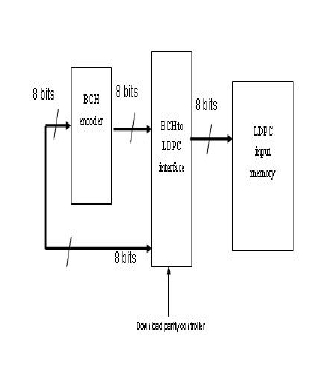
\includegraphics[width = 0.8\linewidth, height= 0.35\textheight]{FECARCH}
\caption{Block diagram of the overall FEC tx section} \label{fig:ovrsys}
\end{figure}

As we shall detail in the next section, the interface between BCH and LDPC is constituted by a simple 8 bits multiplexer together with a suited circuitry to store and download the parity bits after each computation cycle. This interface addresses properly encoded bits into LDPC input memory and it must be driven by a control logic based on clock cycles required (see \tbref{tb:clkreq}) to provide a codeword.

Another important question to raise up is certainly giving the architecture a flexible structure so as to succeed in dealing with each coding rate provided by DVB-S2 FEC. A more versatility, as we shall see, requires an additional usage of memory: as a matter of fact, some additional coefficient of matrices mentioned in the previous chapter must be stored into some LUTs (Look Up Tables).

\begin{table} \centering
\begin{tabular}{||p{2.44cm}||p{2.5cm}||p{2.53cm}||p{2.28cm}||p{2.06cm}||}
\hline
 \multicolumn{1}{|p{2.44cm}|}{\centering BCH Uncoded Block} &  \multicolumn{1}{p{2.5cm}|}{\centering BCH Coded Block \(N\ped{BCH}\)} &  \multicolumn{1}{p{2.53cm}|}{\centering Ticks to transmit informative bits} &  \multicolumn{1}{p{2.28cm}|}{\centering Parity bits download} &  \multicolumn{1}{p{2.06cm}|}{\centering Total clock cycles} \\
\hline
 \multicolumn{1}{|p{2.44cm}|}{\centering 16008} &  \multicolumn{1}{p{2.5cm}|}{\centering 16200} &  \multicolumn{1}{p{2.53cm}|}{\centering 2001} &  \multicolumn{1}{p{2.28cm}|}{\centering 24} &  \multicolumn{1}{p{2.06cm}|}{\centering 2025} \\
 \multicolumn{1}{|p{2.44cm}|}{\centering 21408} &  \multicolumn{1}{p{2.5cm}|}{\centering 21600} &  \multicolumn{1}{p{2.53cm}|}{\centering 2676} &  \multicolumn{1}{p{2.28cm}|}{\centering 24} &  \multicolumn{1}{p{2.06cm}|}{\centering 2700} \\
 \multicolumn{1}{|p{2.44cm}|}{\centering 25728} &  \multicolumn{1}{p{2.5cm}|}{\centering 25920} &  \multicolumn{1}{p{2.53cm}|}{\centering 3216} &  \multicolumn{1}{p{2.28cm}|}{\centering 24} &  \multicolumn{1}{p{2.06cm}|}{\centering 3240} \\
 \multicolumn{1}{|p{2.44cm}|}{\centering 32208} &  \multicolumn{1}{p{2.5cm}|}{\centering 32400} &  \multicolumn{1}{p{2.53cm}|}{\centering 4026} &  \multicolumn{1}{p{2.28cm}|}{\centering 24} &  \multicolumn{1}{p{2.06cm}|}{\centering 4050} \\
 \multicolumn{1}{|p{2.44cm}|}{\centering 38688} &  \multicolumn{1}{p{2.5cm}|}{\centering 38880} &  \multicolumn{1}{p{2.53cm}|}{\centering 4836} &  \multicolumn{1}{p{2.28cm}|}{\centering 24} &  \multicolumn{1}{p{2.06cm}|}{\centering 4860} \\
 \multicolumn{1}{|p{2.44cm}|}{\centering 43040} &  \multicolumn{1}{p{2.5cm}|}{\centering 43200} &  \multicolumn{1}{p{2.53cm}|}{\centering 5380} &  \multicolumn{1}{p{2.28cm}|}{\centering 20} &  \multicolumn{1}{p{2.06cm}|}{\centering 5400} \\
 \multicolumn{1}{|p{2.44cm}|}{\centering 48408} &  \multicolumn{1}{p{2.5cm}|}{\centering 48600} &  \multicolumn{1}{p{2.53cm}|}{\centering 6051} &  \multicolumn{1}{p{2.28cm}|}{\centering 24} &  \multicolumn{1}{p{2.06cm}|}{\centering 6075} \\
 \multicolumn{1}{|p{2.44cm}|}{\centering 51648} &  \multicolumn{1}{p{2.5cm}|}{\centering 51840} &  \multicolumn{1}{p{2.53cm}|}{\centering 6456} &  \multicolumn{1}{p{2.28cm}|}{\centering 24} &  \multicolumn{1}{p{2.06cm}|}{\centering 6480} \\
 \multicolumn{1}{|p{2.44cm}|}{\centering 53840} &  \multicolumn{1}{p{2.5cm}|}{\centering 54000} &  \multicolumn{1}{p{2.53cm}|}{\centering 6730} &  \multicolumn{1}{p{2.28cm}|}{\centering 20} &  \multicolumn{1}{p{2.06cm}|}{\centering 6750} \\
 \multicolumn{1}{|p{2.44cm}|}{\centering 57472} &  \multicolumn{1}{p{2.5cm}|}{\centering 57600} &  \multicolumn{1}{p{2.53cm}|}{\centering 7184} &  \multicolumn{1}{p{2.28cm}|}{\centering 16} &  \multicolumn{1}{p{2.06cm}|}{\centering 7200} \\
 \multicolumn{1}{|p{2.44cm}|}{\centering 58192} &  \multicolumn{1}{p{2.5cm}|}{\centering 58320} &  \multicolumn{1}{p{2.53cm}|}{\centering 7274} &  \multicolumn{1}{p{2.28cm}|}{\centering 16} &  \multicolumn{1}{p{2.06cm}|}{\centering 7290} \\
\hline
\end{tabular}
\caption{Clock cycles required to provide each codeword for each operating mode of DVB-S2} \label{tb:clkreq}
\end{table}

\section{Encoder Description}

A block diagram of BCH encoder architecture is shown in \figref{fig:HWarch}. A brief description on its functioning is given below.
\begin{itemize}
\item All the informative \(k\ped{bch}\) bits enter in parallel (\(p\) bits, i.e., 8 at once), from MSB to LSB, all 192 combinatorial blocks, which perform logic function indicated by \(\vet B_p\) matrix. In other words, each block carries out a row by columns product (over \(GF(2)\)) between the \(i\)-th row of \(\vet B_p\) the \(p\) inputs. Since operations are in GF(2), sums are implementable by XOR gates, multiplications by AND gates. \figref{fig:COMBin} gives a schematic illustration of each combinatorial networks processing \(p\) inputs.
\item  Each flip-flop labelled by \(x_i\) represents a single bit of state vector \(\vet x\) of the system and after exactly \(\frac{k\ped{bch}}{p}\) clock ticks it contains the result of division algorithm.
\item  Combinatorial networks toward the BCH-to-LDPC interface (i.e, on the output side) perform the feedback: each XOR gate is fed by the last \(p\) bits of register state \(\vet x\) (from \(x_{184}\) to \(x_{191}\)) passing through output-combinatorial network described by the two sub-matrices \(\vet C_1\) and \(\vet C_2\) (see \secref{sec:Regularity}). More in details, expression \eqref{eq:Apreg} in \secref{sec:Regularity}, showing an high regularity of \(\vet A^p\), allows to split computation of the first term in \eqref{eq:SEmatr} (i.e, \(\vet A^p \vet x \left[ (i-1)p \right]\)) in two contributes
    \begin{enumerate}
    \item row by column products involving last \(p\) bits of \(\vet x\) and therefore last \(p\) columns of matrix \(\vet A^p\). In other words, the combinatorial networks near to BCH-LDPC interface perform the following product
        \begin{equation} \label{eq:prodotto}
        \left(
        \begin{array}{c}
        \vet C_1 \\
        \vet C_2
        \end{array}
        \right)
        \left(
        \begin{array}{c}
        x_{184}(i) \\
        \vdots \\
        x_{191}(i)
        \end{array}
        \right)
        \end{equation}
     \item 	row by column product involving (starting from bit \(x_8\) of vector \(\vet x\) which correspond to row 9 of matrix \(\vet A^p\)) first \(n-k-p\) bits of vector \(\vet x\) is realized by sum modulo 2 (i.e., XOR gates) nodes on the right of the combinatorial networks. \figref{fig:COMBout} gives a schematic representation of this combinatorial networks together with modulo 2 sum nodes.
     \end{enumerate}
\item Logic functions relevant to sub-matrix \(\vet I\) of \(\vet A^p\) are implemented by XOR gates at the output of combinatorial networks connected to the last \(p\) bits of the state vector.
\item At the end of each computation cycle, the encoder register must be reset.
\end{itemize}

Due to intrinsic simplicity of matrices \(\vet A^p\) and \(\vet B_p\) (they are only composed by zeroes and ones), the two combinatorial networks can be implemented in a very simple way by programmable XOR gates with eight inputs.
More in detail, each coefficient of the above two matrices says which wires have to be connected to each combinatorial network (XOR).


\tikzstyle{8XOR}=[draw, minimum height=9cm, text centered,					
                  inner sep= 0pt, text width= 4em, minimum width= 3cm]

\begin{figure}
\begin{signalflow}[]
\node[input] (i1) {\(x_{184}\)};
\node[input] (i2) [below from=i1] {\(x_{185}\)};
\node[input] (i3) [below from=i2] {\(x_{186}\)};
\node[input] (i4) [below from=i3] {\(x_{187}\)};
\node[input] (i5) [below from=i4] {\(x_{188}\)};
\node[input] (i6) [below from=i5] {\(x_{189}\)};
\node[input] (i7) [below from=i6] {\(x_{190}\)};
\node[input] (i8) [below from=i7] {\(x_{191}\)};
\node[multiplier] (m1) [right from= i1,label=above:\(a_{j\virgola 184}\)] {};
\node[multiplier] (m2) [right from= i2,label=above:\(a_{j\virgola 185}\)] {};
\node[multiplier] (m3) [right from= i3,label=above:\(a_{j\virgola 186}\)] {};
\node[multiplier] (m4) [right from= i4,label=above:\(a_{j\virgola 187}\)] {};
\node[multiplier] (m5) [right from= i5,label=above:\(a_{j\virgola 188}\)] {};
\node[multiplier] (m6) [right from= i6,label=above:\(a_{j\virgola 189}\)] {};
\node[multiplier] (m7) [right from= i7,label=above:\(a_{j\virgola 190}\)] {};
\node[multiplier] (m8) [right from= i8,label=above:\(a_{j\virgola 191}\)] {};
\node[8XOR] (8XOR) [right from=m4] {\Huge XOR};
\node[coordinate] (c1) [right from=8XOR] {};
\node[adder] (a1) [right from=c1] {};
\node[input] (x) [above from=a1, label=above:{\(x_{j-8}(i)\) for \(j \geq 8\)}] {};
\node[output] (out) [right from=a1, label=right:{\(y_j(i)\)}] {};
% signal path
\path[r>] (i1)--(m1);
\path[r>] (i2)--(m2);
\path[r>] (i3)--(m3);
\path[r>] (i4)--(m4);
\path[r>] (i5)--(m5);
\path[r>] (i6)--(m6);
\path[r>] (i7)--(m7);
\path[r>] (i8)--(m8);
\path[r>] (m1) -- +(1,0);
\path[r>] (m2) -- +(1,0);
\path[r>] (m3) -- +(1,0);
\path[r>] (m4) -- +(1,0);
\path[r>] (m5) -- +(1,0);
\path[r>] (m6) -- +(1,0);
\path[r>] (m7) -- +(1,0);
\path[r>] (m8) -- +(1,0);
\path[r] (8XOR) -- (c1);
\path[r>] (x)--(a1);
\path[r>] (c1)--(a1);
\path[r>] (a1)--(out);
\end{signalflow}
\caption{Block scheme of the combinatorial networks acting on the last \(p\) bits of \(\vet x\). \(a_{j \virgola l}\) is the coefficient at \(j\)-th row and \(l\)-th column of \(\vet A^8\) matrix }\label{fig:COMBout}
\end{figure}

\begin{figure}
\begin{signalflow}[]
\node[input] (i1) {\(u(ip-1)\)};
\node[input] (i2) [below from=i1] {\(u(ip-2)\)};
\node[input] (i3) [below from=i2] {\(u(ip-3)\)};
\node[input] (i4) [below from=i3] {\(u(ip-4)\)};
\node[input] (i5) [below from=i4] {\(u(ip-5)\)};
\node[input] (i6) [below from=i5] {\(u(ip-6)\)};
\node[input] (i7) [below from=i6] {\(u(ip-7)\)};
\node[input] (i8) [below from=i7] {\(u[p(i-1)]\)};
\node[multiplier] (m1) [right from= i1,label=above:\(b_{j\virgola 0}\)] {};
\node[multiplier] (m2) [right from= i2,label=above:\(b_{j\virgola 1}\)] {};
\node[multiplier] (m3) [right from= i3,label=above:\(b_{j\virgola 2}\)] {};
\node[multiplier] (m4) [right from= i4,label=above:\(b_{j\virgola 3}\)] {};
\node[multiplier] (m5) [right from= i5,label=above:\(b_{j\virgola 4}\)] {};
\node[multiplier] (m6) [right from= i6,label=above:\(b_{j\virgola 5}\)] {};
\node[multiplier] (m7) [right from= i7,label=above:\(b_{j\virgola 6}\)] {};
\node[multiplier] (m8) [right from= i8,label=above:\(b_{j\virgola 7}\)] {};
\node[8XOR] (8XOR) [right from=m4] {\Huge XOR};
\node[coordinate] (c1) [right from=8XOR] {};
\node[adder] (a1) [right from=c1] {};
\node[input] (x) [above from=a1, label=above:{\(y_{j}(i)\)}] {};
\node[output] (out) [right from=a1, label=right:{\(x_j(i+1)\)}] {};
% signal path
\path[r>] (i1)--(m1);
\path[r>] (i2)--(m2);
\path[r>] (i3)--(m3);
\path[r>] (i4)--(m4);
\path[r>] (i5)--(m5);
\path[r>] (i6)--(m6);
\path[r>] (i7)--(m7);
\path[r>] (i8)--(m8);
\path[r>] (m1) -- +(1,0);
\path[r>] (m2) -- +(1,0);
\path[r>] (m3) -- +(1,0);
\path[r>] (m4) -- +(1,0);
\path[r>] (m5) -- +(1,0);
\path[r>] (m6) -- +(1,0);
\path[r>] (m7) -- +(1,0);
\path[r>] (m8) -- +(1,0);
\path[r] (8XOR) -- (c1);
\path[r>] (x)--(a1);
\path[r>] (c1)--(a1);
\path[r>] (a1)--(out);
\end{signalflow}
\caption{Block scheme representing the combinatorial networks acting on the \(p\) bit of input. \(b_{j \virgola l}\) is the coefficient at \(j\)-th row and \(l\)-th column of the \(\vet B_8\) matrix} \label{fig:COMBin}
\end{figure} 

\section{Dealing with Each Error Protection}

Architecture we have shown as far can only address the greater \(t\) error protection modalities. However, DVB-S2 has been designed to operate in ACM (Adaptive Coding and Modulation) mode, so that a flexible architecture, capable of changing his behavior on a frame basis, would be more desirable.

From our analysis of the two matrices, we have reach the conclusion that they are very regular and, even changing the polynomial generator of the code, this interesting property still holds. The degree of parallelism \(p\), once set by design, cannot vary. Henceforth all our considerations will be constrained to a specific degree of parallelism, \(p=8\), even though the method we are going to show is general at all.

BCH of DVB-S2 provides three protection level \(t = 8\virgola 10 \virgola 12\) associated to the following different generators
\begin{align}
g\ped{t_{12}}(x) & = g_1(x)g_2(x)\ldots g_{12}(x) \label{eq:BCHt12}\\
g\ped{t_{10}}(x) & = g_1(x)g_2(x)\ldots g_{10}(x) \label{eq:BCHt10}\\
g\ped{t_8}(x) & = g_1(x)g_2(x)\ldots g_{8}(x) \label{eq:BCHt8}
\end{align}
where the above polynomials are in \tbref{tb:BCHpoly}.
According to the decrease of the degree of polynomial generator, also the number \(r\) of redundancy bits decreases and thus the number of FFs illustrated in \figref{fig:HWarch} would be oversized. This implies that, \(\vet x\) being changed, size of matrices \(\vet A^8\) and \(\vet B_8\) has to change. In \secref{sec:Regularity} we have shown that, for a reasonable level of parallelism, matrix \(\vet A^p\) shows some regularity. In practice, its structure shown in \eqref{eq:Apreg} does not change from \(t_8\) to \(t_{12}\), although its coefficients are, of course, subject to variations. Same consideration can be made upon \(\vet B_p\) matrix, which however shows no regularity property for this kind of architecture.

\figref{fig:COMBin} and \figref{fig:COMBout} clearly show that these kind of combinatorial network are programmable by means of their coefficients, determining which wire has to be connected to the 8-inputs XOR gate and which not. Imposing, for example, that all of these coefficients are forced to zero, we would get the result of having inhibited the \(j\)-th combinatorial network. This is exactly what we can do to deal with all the protection level \(t\).

In particular, either \(\vet A^8\) or \(\vet B_8\) can be embedded into the their largest matrices of size, respectively, \(192 \times 192\) and \(192 \times 8\) in this way:
\begin{description}
\item[Medium Protection Level](\(t=10\)) Matrices \((\vet A^8)\ped{o}\) and \((\vet B_8)\ped{o}\) oversized (they should be \(160 \times 160\) and \(160 \times 8\) respectively) turn out to be as follows
    \begin{align}
    (\vet A^8)\ped{o} &=
    \left(
    \begin{array}{cc}
    \vet 0 & \vet 0 \\
    \vet 0 & (\vet A^8)\ped{t_{10}}
    \end{array}
    \right) &
    (\vet B_8)\ped{o} &=
    \left(
    \begin{array}{c}
    \vet 0 \\
    (\vet B_8)\ped{t_{10}}
    \end{array}
    \right)
    \end{align} \label{eq:embedding}
    This corresponds to inhibit the first 32 couples of combinatorial networks since their coefficients are all nulls. Thus, all the first 32 FFs (from \(x_0\) to \(x_{31}\)) of the BCH encoder will contain always zeroes.
\item[Low Protection Level](\(t=8\)) The oversized matrices are build in the same manner and now the first 64 couples of combinatorial networks are inhibited since their coefficients are all nulls.
\end{description}

\begin{figure} \centering
%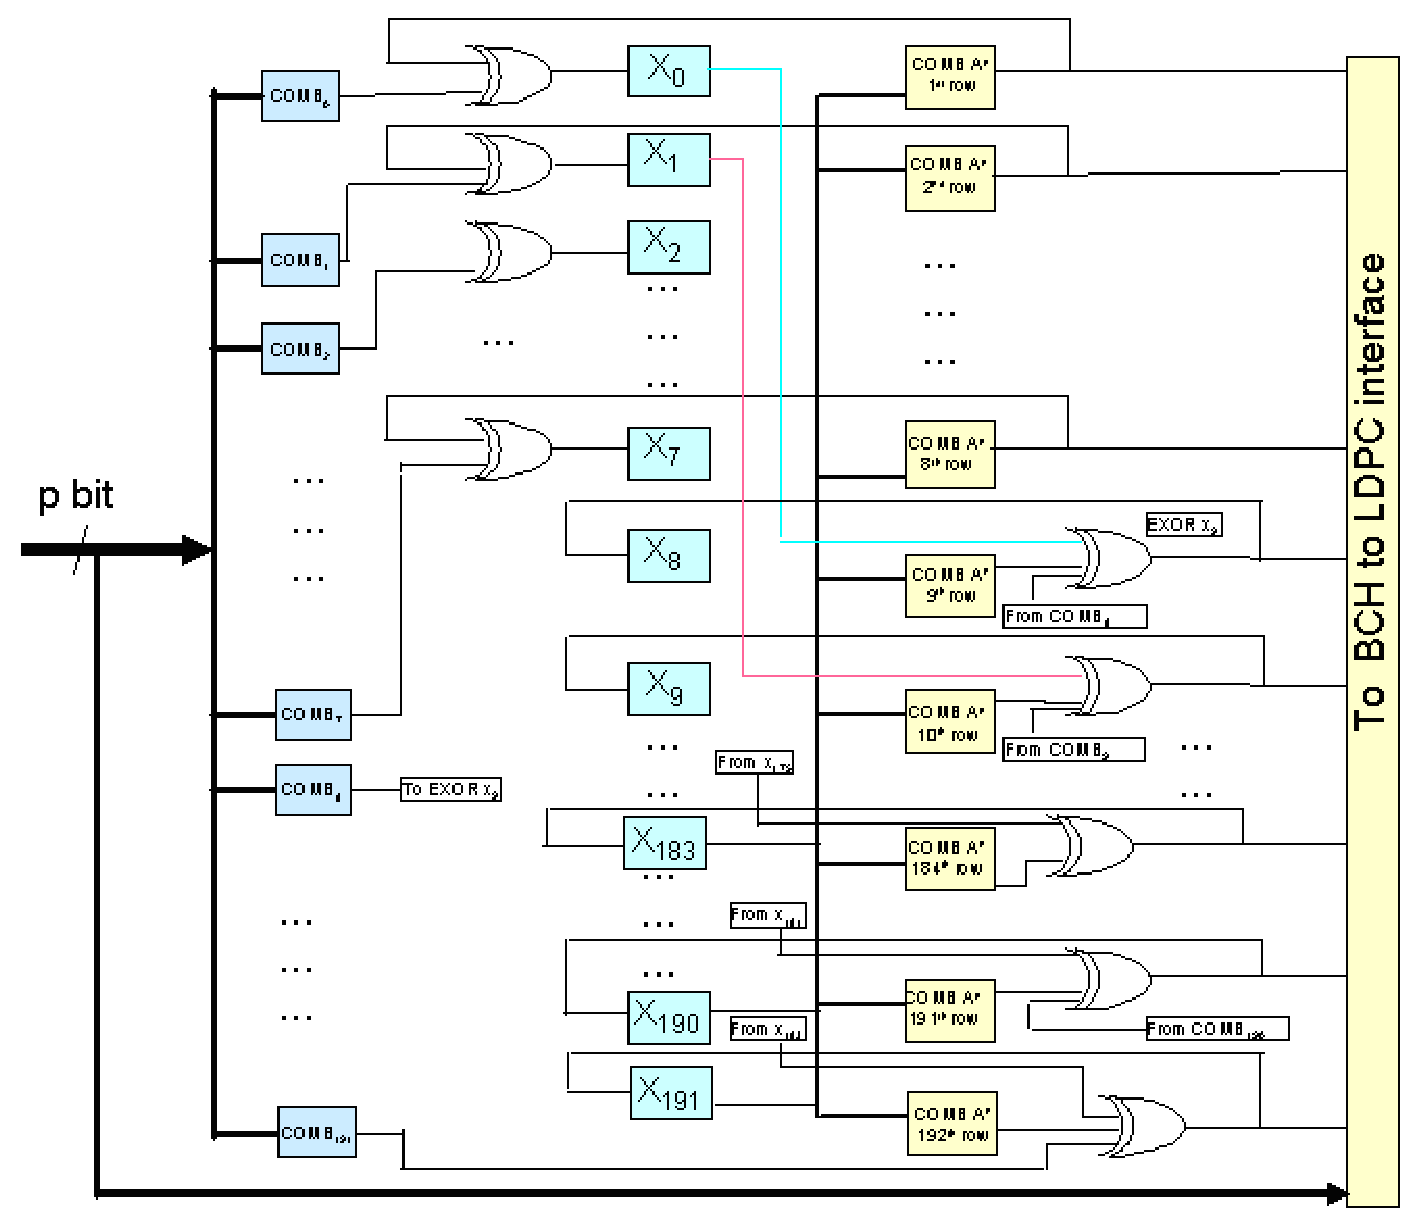
\includegraphics[width = 0.8\linewidth, height= 0.8\textheight]{encblock}
\tikzstyle{BUS}
 = [line width=2pt,
      >= real tip,
      draw]
\tikzstyle{phan}
  = [minimum size=\delaysize]
\begin{signalflow}[node distance=1cm]
\node[coordinate] (c1)  {};
%
%\node[coordinate] (c183) [below from=c182] {};
%\node[coordinate] (c184) [below from=c183] {};
%\node[coordinate] (c186) [below from=c184] {};
%\node[coordinate] (c191) [below from=c186] {};
%% Input Combinatorials
\node[delay] (a1)  [right from=c1] {\(\vet b_1 \vet u\)};
\node[delay] (a2) [below from=a1] {\(\vet b_2 \vet u\)};
\node[phan] (a3) [below from=a2] {\(\vdots\)};
\node[delay] (a8) [below from=a3] {\(\vet b_8 \vet u\)};
\node[delay] (a9) [below from=a8] {\(\vet b_9 \vet u\)};
\node[phan]  (phh) [below from=a9] {\(\vdots\)};
\node[delay] (a183) [below from=phh] {\(\vet b_{184} \vet u\)};
\node[delay] (a184) [below from=a183] {\(\vet b_{185} \vet u\)};
\node[phan] (a186) [below from=a184] {\(\vdots\)};
\node[delay] (a191) [below from=a186] {\(\vet b_{192} \vet u\)};
%% Some coordinates
\node[coordinate] (c2) [left from=a2] {};
\node[coordinate] (c3) [left from=a8] {};
\node[coordinate] (c4) [left from=a9] {};
\node[coordinate] (c9) [below from=c4, below=2.37cm] {};
\node[coordinate] (c182) [below from=c9,below=.63cm] {};
\node[coordinate] (c183) [left from=a191, right=.14cm] {};

\node[coordinate] (input) [left from=c9] {};
%% First XORs stage
\node[adder]  (x1) [right from=a1, left=0cm] {};
\node[adder]  (x2) [right from=a2,left=0cm] {};
\node[adder]  (x8) [right from=a8,left=0cm] {};
\node[adder]  (x9) [right from=a9,left=0cm] {};
\node[adder]  (x183) [right from=a183,left=0cm] {};
\node[adder]  (x184) [right from=a184,left=0cm] {};
\node[adder]  (x191) [right from=a191,left=0cm] {};
%% Feedbacks
\node[input]  (i1) at (x1) [above= .65cm,label=right:{\(y_0\)}] {};
\node[input]  (i2) at (x2) [above= .65cm,label=right:{\(y_1\)}] {};
\node[input]  (i8) at (x8) [above= .65cm,label=right:{\(y_7\)}] {};
\node[input]  (i9) at (x9) [above= .65cm,label=right:{\(y_8\)}] {};
\node[input]  (i183) at (x183) [above= .65cm,label=right:{\(y_{183}\)}] {};
\node[input]  (i184) at (x184) [above= .65cm,label=right:{\(y_{184}\)}] {};
\node[input]  (i191) at (x191) [above= .65cm,label=right:{\(y_{191}\)}] {};
%% Register of state
\node[delay]  (s1) [right from=x1] {\(x_0\)};
\node[delay]  (s2) [right from=x2] {\(x_1\)};
\node[delay]  (s8) [right from=x8] {\(x_7\)};
\node[delay]  (s9) [right from=x9] {\(x_8\)};
\node[phan]   (ph) [below from=s9] {\(\vdots\)};
\node[delay]  (s183) [below from=ph] {\(x_{183}\)};
\node[delay]  (s184) [below from=s183] {\(x_{184}\)};
\node[phan] (sp) [below from=s184] {\(\vdots\)};
\node[delay]  (s191) [below from=sp] {\(x_{191}\)};

%% Outputs
\node[output] (so1) [right from=s1] {};
\node[output] (so2) [right from=s2] {};
\node[output] (so8) [right from=s8] {};
\node[output] (so9) [right from=s9] {};
\node[output] (so183) [right from=s183, left=0cm] {};

%% Bus on the right side
%\node[coordinate] (cc184) [right from=s191] {};
%\node[coordinate] (cc9) [above from=cc184] {};
%\node[coordinate] (cc8) [above from=cc9] {};
%\node[coordinate] (cc2) [above from=cc8] {};
%\node[coordinate] (cc7) [above from=cc8] {};
%\node[coordinate] (cc6) [above from=cc7] {};
%\node[coordinate] (cc3) [above from=cc6] {};
%\node[coordinate] (cc2) [above from=cc3] {};
%\node[coordinate] (cc1) [above from=cc2] {};
\node[coordinate] (cc191) [right from=s191, right=1cm] {};
\node[coordinate] (cc186) [right from=s184, right=1cm] {};
\node[coordinate] (cc183) [right from=s183, right=1cm] {};
\node[coordinate] (cc9)   [right from=s9, right=1.15cm] {};
\node[coordinate] (cc8)  [right from=s8, right=1.15cm] {};
\node[coordinate] (cc2) [right from=s2, right=1.15cm] {};
\node[coordinate] (cc1) [right from=s1, right=1.15cm] {};

%% Cominatorial networks on the right side
\node[delay] (b1) [right from=cc1] {};
\node[delay] (b2) [right from=cc2] {};
\node[phan] (b3)  [below from=b2] {\(\vdots\)};
\node[delay] (b4) [right from=cc8] {};
\node[delay] (b5) [right from=cc9] {};
\node[delay] (b6) [right from=cc183] {};
\node[delay] (b7) [right from=cc186] {};
\node[delay] (b8) [right from=cc191] {};

%% At the output of the above combinatorial
\node[output] (n1) [right from=b1, label=right:{\(y_0\)}, right=1cm] {};
\node[output] (n2) [right from=b2, label=right:{\(y_1\)}, right=1cm] {};
\node[output] (n3) [right from=b4, label=right:{\(y_7\)}, right=1cm] {};
\node[adder]  (n4) [right from=b5] {};
\node[output] (n4b) [right from=n4, label=right:{\(y_8\)}]  {};
\node[adder]  (n5) [right from=b6] {};
\node[output] (n5b) [right from=n5, label=right:{\(y_{183}\)}]  {};
\node[adder]  (n6) [right from=b7] {};
\node[output] (n6b) [right from=n6, label=right:{\(y_{184}\)}]  {};
\node[adder]  (n7) [right from=b8] {};
\node[output] (n7b) [right from=n7, label=right:{\(y_{191}\)}]  {};

\node[input]  (ii4) at (n4) [above= .65cm,label=right:{\(x_0\)}] {};
\node[input]  (ii5) at (n5) [above= .65cm,label=right:{\(x_{175}\)}] {};
\node[input]  (ii6) at (n6) [above= .65cm,label=right:{\(x_{176}\)}] {};
\node[input]  (ii7) at (n7) [above= .65cm,label=right:{\(x_{183}\)}] {};
%\node[input]  (i183) at (x183) [above= .65cm,label=right:{\(y_{183}\)}] {};
%\node[input]  (i184) at (x184) [above= .65cm,label=right:{\(y_{184}\)}] {};
%\node[input]  (i191) at (x191) [above= .65cm,label=right:{\(y_{191}\)}] {};

%%% BUS WIRES
\path[BUS] (c1)--(c2)--(c3)--(c4)--(c9)--(c182)--(c183)
            (c1)--(a1)
            (c2)--(a2)
            (c3)--(a8)
            (c4)--(a9)
            (c9)--(a183)
            (c183)--(a191)
            (c182)--(a184);
\path[BUS]  (cc191)--(cc183)--(cc9)--(cc8)--(cc2)--(cc1);


%%% COMB1 to adder connections
\path[r>]   (a1)--(x1);
\path[r>]   (a2)--(x2);
\path[r>]   (a8)--(x8);
\path[r>]   (a9)--(x9);
\path[r>]   (a183)--(x183);
\path[r>]   (a184)--(x184);
\path[r>]   (a191)--(x191);

%%%% State register outputs
\path[r>]   (s1)--(so1);
\path[r>]   (s2)--(so2);
\path[r>]   (s8)--(so8);
\path[r>]   (s9)--(so9);
\path[r>]   (s183)--(so183);

%%% First adders stage to state ragister connections
\path[r>]   (x1)--(s1);
\path[r>]   (x2)--(s2);
\path[r>]   (x8)--(s8);
\path[r>]   (x9)--(s9);
\path[r>]   (x183)--(s183);
\path[r>]   (x184)--(s184);
\path[r>]   (x191)--(s191);

%% Feedback connections to the first adders stage
\path[r>]   (i1)--(x1);
\path[r>]   (i2)--(x2);
\path[r>]   (i8)--(x8);
\path[r>]   (i9)--(x9);
\path[r>]   (i183)--(x183);
\path[r>]   (i184)--(x184);
\path[r>]   (i191)--(x191);

%% Feedforward connection to the last adders stage
\path[r>]   (ii4)--(n4);
\path[r>]   (ii5)--(n5);
\path[r>]   (ii6)--(n6);
\path[r>]   (ii7)--(n7);

%% Last 8 FFs of X to BUS
\path[r]  (s184)--(cc186)
          (s191)--(cc191);

%%% COMB2 to out/adders connections
\path[r>]  (b1)--(n1);
\path[r>]  (b2)--(n2);
\path[r>]  (b4)--(n3);
\path[r>]  (b5)--(n4);
\path[r>]  (b6)--(n5);
\path[r>]  (b7)--(n6);
\path[r>]  (b8)--(n7);

%%% Last adders to output
\path[r>]  (n4)--(n4b);
\path[r>]  (n5)--(n5b);
\path[r>]  (n6)--(n6b);
\path[r>]  (n7)--(n7b);

%%% Right Hand BUSES
\path[BUS] (cc1)--(b1)
           (cc2)--(b2)
           (cc8)--(b4)
           (cc9)--(b5)
           (cc183)--(b6)
           (cc186)--(b7)
           (cc191)--(b8);
\end{signalflow} 
\caption{Architecture oriented to digital hardware implementation. Each combinatorial network on the left-hand side implements a row by column product of \(\vet B_8 \vet u\). Each row of matrix \(\vet B_8\) is indicated as \(\vet b_j\) with \(0\leq j<192\). Each combinatorial network on the right-hand side implements a row by column sub-product in \eqref{eq:prodotto}. The 8 bit bus on the input side carries message bits to be encoded.} \label{fig:HWarch}
\end{figure}


\section{Interface and Parity Bits Extraction}

The interface between BCH and LDPC encoder can be implemented as illustrated in \figref{fig:Interface}. The parity bits, once computed (at \(n\ped{bch}\) clock tick), can be saved (in a single clock cycle) in a shift register architecture, which has been called in \figref{fig:Interface} 192 (or rather, up to 192) to 8 bit converter. In fact, its task is formatting data in the DVB-S2 format. Furthermore, this kind of architecture allows to write all the parity bits extracted from BCH encoder (in a single clock tick) into LDPC input memory with a degree of parallelism equal to 8\footnote{Note also that \(p=8\) is not only a divisor for 360, but also for 192(\(t=12\)), 160(\(t=10\)) and 128(\(t=8\))}.

Further detailing, the converter is composed by 8 shift register blocks with size equal to 24 bits. In a preliminary fase all the parity bits computed by the BCH encoder are stored in these blocks following the labelling indicated in \figref{fig:Download} (to succeed in storing these bits, MUXs between each flip flop can be used). Afterward, the converter works as a shift register, thus allowing to download data eight at once, i.e., with a degree of parallelism equal to 8.

To summarize, let us see, in order for each iteration, the operations carried out by this specific interface:

\begin{enumerate}
\item Once the parity bits have been computed, they are stored in another shift register according to the bit-to-bit mapping illustrated in \figref{fig:Download}. MUXs between a FF and its neighbor allow to store bits all at once (in parallel) as they are switched on wires carrying results of encoding (these wires may be directly connected to the BCH encoder register).
\item As MUXs are switched on wires interconnecting FFs each other, all the bits previously stored, shifting along FFs, are carried by some 'strategic' wires on the 8 bits bus, which conveys parity bits toward the output multiplexer.
    Practically, the register is working as a shift register.
\item The output multiplexer has two inputs buses connected to: informative bits and redundancy bits. MUX should be driven by a proper control logic on the operating mode basis.
\end{enumerate}



\begin{figure} \centering
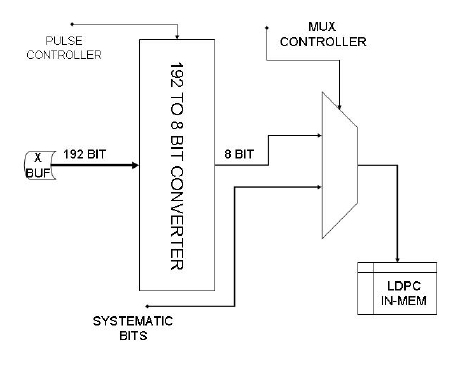
\includegraphics[scale=0.8]{Interface}
\caption{Interface architecture. Parity bits are loaded into the 192 to 8 bits converter.} \label{fig:Interface}
\end{figure}


\begin{figure} \centering
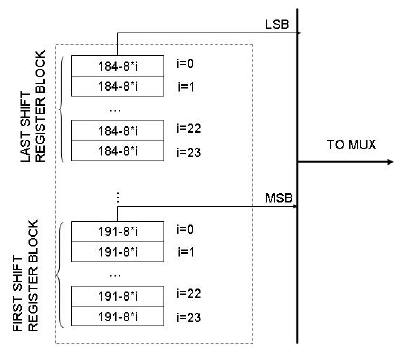
\includegraphics[scale=1]{download}
\caption{192 to 8 bits converter architecture. Values into each FF represent the index mapping between the BCH encoder register and the interface register, used to extract and format data.} \label{fig:Download}
\end{figure}


\section{Frequency and Memory Requirements}

Taking into account LDPC outer encoder frequency requirements and imposing a data rate equal to \(1 \unit{Gbps}\), in the worst case, that is, when \(t=8\) and LDPC code rate is equal to \(9/10\), we obtain the maximum frequency requirement so as to guarantee this challenging performance:
\begin{equation}
(f\ped{clk})\ped{MAX}= \frac{frame}{s}\cdot 7290 = 125 \unit{MHz}
\end{equation}
Concerning to memory requirement either, the architecture proposed takes six (two per each level of BCH protection parameter \(t\)) LUTs to store coefficients used by the combinatorial networks. As a matter of fact, storing of the \(\vet C_1\) and \(\vet C_2\) sub-matrices (recall that they represent two sub-blocks, whose aggregated size is \(192 \times 8\), of the \(\vet A^8\) matrix) coefficients as well matrix \(\vet B_8\), whose size is \(192 \times 8\), coefficients is required. To provide an encoder capable of dealing with each \(t\)-error protection level, those matrices have to be saved in LUTs for each \(t\).
The size of each LUT is equal to \(192 \unit{Bytes}\) and thus the BCH encoder, apart from additional memory required by the BCH-LDPC interface and the encoder state register, requires an amount of memory equal to
\begin{equation}
 2\cdot3\cdot192\unit{B} = 1,125\unit{KiB}.
\end{equation}


\chapter{Software Package for VHDL Validation} \label{ch:SWForVDL}
%Goal of this Chapter is to show results provided by simulations aimed at verifying the good functioning of algorithms and architecture proposed. At a first stage, it will be proved that encoder makes its work encoding any bitstream in a proper way through a ; at a second stage,


\section{Software Implementation of Serial Encoder}

This section describes the software implementations of the architecture illustrated in \figref{fig:SerEnc}. Recall that only this architecture is actually serial since the other one (depicted in \figref{fig:PolyDiv}), which computes parity bits in \(n\ped{bch}\) clock ticks, needs a parallel fetching of the encoding result and a reset of the register at the end of each computation cycle\footnote{Clearly, in software, this distinction is not so strict}.

The software implementation shown below simulates the serial architecture depicted in \figref{fig:SerEnc}. For the first \(k\) clock ticks, the informative bits exits while the feedback loop is enabled. From \(k\) to \(n\) instead, the feedback loop is disabled and then all the parity bits ready to be fetched are carried (serially) to the output while zeros are going to be stored into each stage of the shift register, thus resetting the register. This is certainly an advantage with respect to architecture depicted in \figref{fig:PolyDiv}, which requires a parallel fetching of the parity bits together with, in turn, a reset of the shift register.

To simulate the two different behaviors of the serial encoder, which for \(k\) clock cycles yields the bits of message while for the next one produces the parity bits, a integer \texttt{encStep} counter has been employed. It follows a useful description of the used variable:
\begin{itemize}
\item \texttt{ticks} is a function parameter and refers to the numbers of iteration/clock-ticks which have to be simulated; \texttt{m[], out[]}, other ones function parameters, are vector relevant to input and output. The function \texttt{Run} reads from \texttt{m[]} and write in turn the result of \texttt{ticks} computation cycles.
\item Vector of integer \texttt{state[]} represent the values contained in each register of the encoder.
\item \texttt{g[]} represent in vectorial form polynomial generator of the BCH code.
\item \texttt{r} is the length of the shift register.
\end{itemize}

%\listing{serial.c}
%\lstinputlisting[caption={[senc]BCH Serial Encoder}]{serenc.c}
\lstinputlisting{serial.c}
This piece of software works serially, but the user may define the number of iterations that emulator machine has to perform. Anyway this software emulator, as its more physical version, takes \(n\) clock ticks to encode a single codeword.

\section{Software Implementations of Parallel Encoder}

Matrices \(\vet A^8\) and \(\vet B_8\) defined in \secref{sec:Regularity} have been pre-computed via software by a Matlab routine. Useful coefficients of these matrices can be stored in local variables (software) or in LUT (hardware). Note that, concerning the \(\vet A^8\) matrix, the sub-matrices \(\vet C_1\) and \(\vet C_2\) should be stored in a dedicated memory for each t-error correction level to make the architecture flexible.

The first software implementation refers to the slower parallel architecture which spends \(n\) clock ticks to provide codewords associated to messages. Pre-computed parts of the matrix \(\vet A^8\) relevant to each operating modes are loaded and saved in memory on \( (n \virgola k) \) (only those provided by the standard) basis. Matrix \(\vet B_p\), already defined in \eqref{eq:Btrivial} (see also the example in \secref{sec:Regularity}), is trivial and its save in memory can be avoided since that form corresponds to connect the eight inputs to the first XOR stage of the architecture. In other words, the 192 combinatorial networks on the input side (depicted in \figref{fig:HWarch}) in this kind of architecture are not necessary.
The following function is dedicated to simulate the functioning of combinatorial networks on the output side:
%\begin{itemize}
%\item Input combinatorial network acting on the eight inputs and entering each XOR gate together with the feedback wire. Function \texttt{combc(index, input)} provides the result of row by column product between matrix \(\vet B_8\) and inputs.
%\item Feedback combinatorial network acting on the last eight values of the state register. Function \texttt{combn(index, n, regold)} implements the product row by column between \(\vet C_1 \virgola \vet C_2\) and \(x_{184}\virgola \ldots \virgola x_{191}\).
%\end{itemize}
\begin{itemize}
\item Feedback combinatorial network acting on the last eight values of the state register. Function \texttt{combn(index, n, regold)} implements the product row by column between \(\vet C_1 \virgola \vet C_2\) and \(x_{184}\virgola \ldots \virgola x_{191}\).
\end{itemize}

\lstinputlisting{comb1.c}

%As we shall see in the description of technology solution adopted to implement via hardware the BCH encoder, we hav
The first part of function \texttt{BCHnclkpar(int n,int k)} is relevant to the error protection level and consequently due to the state vector allocation (recall that register length can be 128, 160, 192 with respect to \(t = 8 \virgola 10 \virgola 12\) possible values). In case of mismatch with the couples \(n \virgola k\), provided by the standard DVB-S2 for the normal FECFRAME, simulation is aborted.
The \texttt{for} cycle in the middle part of the program updates cyclically the register of the encoder, using the above function implementing each combinatorial networks. %To prevent that combinatorial networks deal with register values relevant to the future,
Eventually, output is formatted in the systematic form complyant with the DVB-S2 standard requirements.

\lstinputlisting{parnclk.c}


The second implementation is connected to the faster architecture (its correspondent serial version is depicted in \figref{fig:SerEnc}) which spends \(k\) clock ticks to compute parity bits, saving, compared to the first, \(r\) clock cycles for each computation cycle or, i.e., for each encoding cycle. The function \texttt{combn(index, n, regold)} implementing the combinatorial networks on the output side is the same of the slower architecture according to what we said in Chapter \ref{ch:BCHAlg&Arch} (i.e. matrix \(\vet A_8 \) cannot change).
Therefore here we have two functions:
\begin{itemize}
\item Function \texttt{combc(index, input)} provides the result of row by column product between matrix \(\vet B_8\) and the inputs.
\item  Function \texttt{combn(index, n, regold)} implements the product row by column between \(\vet C_1 \virgola \vet C_2\) and \(x_{184}\virgola \ldots \virgola x_{191}\).
\end{itemize}

\lstinputlisting{comb2.c}

\lstinputlisting{parkclk.c}

\section{Galois Fields Tables}

As said in \secref{sec:BCHstruct}, the knowledge of the big field \(GF(2^{16})\) where the roots of polynomial generators are is necessary to make error detection and decoding (e.g. by Berlekamp-Massey Algorithm). Galois field associated to this BCH code can be built by using \(g_1(x)\) in \tbref{tb:BCHpoly}, which is also the primitive polynomial of \(GF(2^{16})\) for the reasons already expressed in \secref{sec:BCHstruct}.

All the \(2^{16}-1\) elements of this field can be obtained by a LFSR structure (implementing the division algorithm as that depicted in \figref{fig:PolyDiv}) where each connection/disconnection (since we are over GF(2)) corresponds to coefficients of \(g_1(x)\). This LFSR architecture, however, performs all their operations in absence of external stimulus (i.e, the single input \(u(i)\) is forced to zero \(u(i) = 0\)).
%This structure is also an optimal pseudo-noise source since generates maximum length sequences.
The state evolution repeats for each multiple of \(2^{16}-1\): if the shift register is initialized by a unitary seed (\(0\virgola \ldots \virgola 0 \virgola 1 \)), then we will find the same seed after \(2^{16}-1\) clock ticks. This means that the initialization seed is a primitive element of GF(\(2^{16}\)).
Each primitive element can be found by trial end errors:according to Definition A.3.2, when an initialization seed leads to have a 1 at \(2^{16}-1\) clock tick, then a primitive element has been found, otherwise it does not. In our simulation, for the sake of simplicity, \(\alpha = 1\) has been used as primitive element.

\lstinputlisting{gfield.c}

At each clock cycle (evolution of the shift-register state) two tables are written down: \begin{enumerate}
\item Each \(\alpha^i\) for \(i = 1\virgola \ldots \virgola 2^{16}-2\) is stored in the \texttt{powOfAlpha[i]} vector/table.
\item Inverse of the \texttt{powOfAlpha[i]} vector/table is saved in the vetor/table
\texttt{index\-Al\-pha[i]} which, given the \(\alpha^i\) value (in decimal notation), provides the correspondent exponent of primitive element \(\alpha\). In practice, this vector/table expresses a base \(\alpha\) logarithm (i.e. \(\log_{\alpha}\) operator).
\end{enumerate}
Usefulness of these two vector/tables will be made clear later on.

\section{Decoding BCH}

Algebraic decoding of a binary BCH code consists of the following steps:
\begin{enumerate}
\item Computation of syndrome (this is implemented by \texttt{errordetection} function).
\item Determination of an \emph{error locator polynomial}, whose roots provide an indication of where the errors are. There are two ways of finding the locator polynomial: Peterson's algorithm and the Berlekamp-Massey algorithm (used in our simulations). In addition, there are techniques based on Galois-field Fourier transforms.
\item Finding the roots of the error locator polynomial. Usually, this is done using the \emph{Chien search}, which is an exhaustive search over all elements in the field.
\end{enumerate}

\subsection{Error Detection}
Before trying to decode a BCH codeword, a preliminary error detection must be accomplished. Parity check \eqref{eq:pchk} evaluation in the \(2t\) roots of polynomial generator provides the code syndrome
\begin{equation} \label{eq:syndr}
\vet S = S_1 = c(\alpha) \virgola S_2 = c(\alpha^2) \virgola \ldots \virgola S_{2t} = c(\alpha^{2t})
\end{equation}
If the codeword received has not been corrupted by noise, then the syndrome is null since \(g(\alpha) = g(\alpha^2) = \ldots = g(\alpha^{2t})\); otherwise it is not and then the decoding should be accomplished to exploit redundancy introduced and try to correct errors occurred. Values in \eqref{eq:syndr} lie over \(GF(2^{16})\) and all the decoding operations have to be carried out in the Galois field where the roots are.

\lstinputlisting{errdet.c}

To evaluate the \(2t\) equations relevant to the syndrome, the tables/vectors pre-computed (because roots are always in \(GF(2^{16})\), given that BCH code is \emph{shortened}) are necessary to compute the \(2t\) syndromes. In fact, the function \texttt{errordetection()} takes as parameters \texttt{powOfAlpha[], indexAlpha[]} vectors. They are useful to
\begin{itemize}
\item compute products among elements of \(GF(2^{16}) \) expressed in exponential form (recall that each element in Galois fields can be written as any power of any primitive element), exploiting exponential properties which still hold in finite fields;
\item find the correspondent power of the primitive element which represents, for example, the sum between two elements of GF (e.g. \( \alpha^2 + \alpha^{11}\)).
\end{itemize}

If any error is detected (i.e. \texttt{syn} is \texttt{true}) then the codeword corrupted can be corrected using the Berlekamp-Massey algorithm.

\subsection{Berlekamp-Massey Algorithm}

Before giving a brief description of the algorithm, let us introduce some notation and mathematical concept. Returning to \eqref{eq:syndr}, suppose that \(\vet r\), the received vector, contains \(\nu\) errors in locations \( i_1 \virgola i_2 \virgola \ldots \virgola i_{\nu}\) so that each element of \(\vet S\) can be rewritten as
\begin{equation}
S_j = \sum_{l =1}^{\nu} {{(\alpha^j)}^{i_l}} = \sum_{l =1}^{\nu} {{(\alpha^{i_l})}^j}
\end{equation}
Letting \(X_l = \alpha^{i_l}\), we obtain the following \(2t\) equations
\begin{equation}
S_j = \sum_{l =1}^{\nu} {{X_l}^j} \qquad j = 1\virgola 2\virgola \ldots \virgola 2t
\end{equation}
in the \(\nu\) unknown error locators. In principle this set of nonlinear equations could be solved by an exhaustive search, but this would be computationally expensive or intractable.
To overcome this problem, a new polynomial is introduced, the \emph{error locator polynomial} which casts the problem in a different, and more tractable, setting.

The error locator polynomial is defined as
\begin{equation} \label{eq:elp}
\Lambda(x) = \prod_{l = 1}^{\nu} {(1-X_lx)} = \Lambda_{\nu}x^{\nu} + \ldots +\Lambda_1x + \Lambda_0
\end{equation}
where \(\Lambda_0 = 1\). In practice, the roots of \eqref{eq:elp} are at the reciprocals of the error locators.

It is possible to demonstrate (for this proof and further information see \cite{b:moon}) that there exist a linear feedback shift register relationship between the syndromes and the coefficients of the error locator polynomial. In practice, we can write
\begin{equation} \label{eq:SynLocLFSR}
S_j = - \sum_{i = 1}^{\nu} {\Lambda_i S_{j-i}} \qquad j = \nu+1 \virgola \nu + 2 \virgola \ldots \virgola 2t
\end{equation}
This formula describes the output of a linear feedback shift register (LFSR) with coefficients \(\Lambda_1 \virgola  \Lambda_2 \virgola \ldots \virgola \Lambda_{\nu} \). From this point of view, the decoding problem consists of finding \(\Lambda_j\) coefficients in such a way that the LFSR generates the known sequence of syndromes \(S_1\virgola S_2\virgola \ldots \virgola S_{2t}\).

In the Berlekamp-Massey algorithm, we build the LFRS that produces the entire sequence \( \{S_1\virgola S_2\virgola \ldots \virgola S_{2t} \}\) by successively modifying an existing LFSR, if necessary to produce increasingly longer sequences. Clearly, we start with an LFRS that could produce \(S_1\). We determine if that LFRS could also produce the sequence \( \{S_1\virgola S_2\}\); if it can, then no modifications are necessary. If the sequence cannot be produced using the current LFSR configuration, we determine a new LFRS that can produce the longer sequence. Proceeding inductively in this way, we start from an LFSR capable of producing the sequence \( \{S_1\virgola S_2\virgola \ldots \virgola S_{k-1} \}\) and modify it, if necessary, so that it can also produce the sequence \( \{S_1\virgola S_2\virgola \ldots \virgola S_{k} \}\). At each stage, the modification to the LFRS are accomplished so that the LFSR is the shortest possible. By this means, after completion of the algorithm an LFSR has been found that is able to produce \( \{S_1\virgola S_2\virgola \ldots \virgola S_{2t} \}\) and its coefficients correspond to the error locator polynomial \(\Lambda(x)\) of smallest degree.

Since we build up the LFSR using information from prior computations, we need a notation to represent the \(\Lambda(x)\) used at different stages of algorithm. Let \(L_k\) denote the length of LFSR produced at stage \(k\) of the algorithm. Let
\begin{equation}
\Lambda^{[k]}(x) = 1 + \Lambda_1^{[k]}x + \cdots + \Lambda_{L_k}^{[k]}x^{L_k}
\end{equation}
be the \emph{connection polynomial} at stage \(k\), indicating the connections for the LFSR capable of producing the output sequence \(\{S_1\virgola S_2\virgola \ldots \virgola S_{k} \}\). That is,
\begin{equation}
S_j = - \sum_{i = 1}^{L_k} {\Lambda_i^{[k]} S_{j-i}} \qquad j = L_k+1 \virgola L_k + 2 \virgola \ldots \virgola k
\end{equation}

At some intermediate step, suppose we have a connection polynomial \(\Lambda^{[k-1]}(x)\) of length \(L_{k-1}\) that produces \( \{S_1\virgola S_2\virgola \ldots \virgola S_{k-1} \}\) for some \(k-1 < 2t\). We check if this connection polynomial also produces \(S_k\) by computing the output
\begin{equation}
\hat{S_k} = - \sum_{i = 1}^{L_k-1} {\Lambda_i^{[k-1]} S_{k-i}}
\end{equation}
If \(\hat{S_k}\) is equal to \(S_k\), then there is no need to update the LFSR, so \(\Lambda^{[k]}(x)= \Lambda^{[k-1]}(x)\) and \(L_k=L_{k-1}\). Otherwise, there is some nonzero \emph{discrepancy} associated with \(\Lambda^{[k-1]}(x)\),
\begin{equation} \label{eq:discrepancy}
d_k = S_k - \hat{S_k} = S_k + \sum_{i = 1}^{L_k-1} {\Lambda_i^{[k-1]} S_{k-i}} =
\sum_{i = 0}^{L_k-1} {\Lambda_i^{[k-1]} S_{k-i}}
\end{equation}
In this case we can update the connection polynomial using the formula
\begin{equation}
\Lambda^{[k]}(x) = \Lambda^{[k-1]}(x) + A x^l \Lambda^{[m-1]}(x)
\end{equation}
where \(A\) is some element in the field, \(l\) is an integer, and \(\Lambda^{[m-1]}(x)\) is one of the prior connection polynomials produced by our process associated with nonzero discrepancy \(d_m\).
Using this new connection polynomial, we compute the new discrepancy, denoted by \({d_k}'\), as
\begin{align}
{d_k}' &= \sum_{i = 0}^{L_k} {\Lambda_i^{[k]} S_{k-i}}\\
     &= \sum_{i = 0}^{L_k-1} {\Lambda_i^{[k-1]} S_{k-i}} + A \sum_{i = 0}^{L_m-1} {\Lambda_i^{[m-1]} S_{k-i-l}} \label{eq:discrep2}
\end{align}
Now, let \(l=k-m\). Then, by comparison with the definition of the discrepancy in \eqref{eq:discrepancy}, the second summation gives
\begin{equation}
A \sum_{i = 0}^{L_m-1} {\Lambda_i^{[m-1]} S_{m-i}} = A d_m
\end{equation}
Thus, if we choose \(A=-d_m^{-1}d_k\), then the summation in \eqref{eq:discrep2} gives
\begin{equation}
{d_k}' = d_k -d_m^{-1} d_k d_m = 0
\end{equation}
So the new connection polynomial produces the sequence \( \{S_1\virgola S_2\virgola \ldots \virgola S_{k} \}\) with no discrepancy. We do not investigate here on how to find the shortest LFSR reproducing syndromes with no discrepancy. We assume that below algorithm could do that. For a complete treatment on LFSR length in Massey algorithm see \cite{b:moon}.

Algorithm shown below use the following variables
\begin{itemize}
\item Vectors/tables \texttt{pow}, \texttt{index} to simplify multiplications among the elements of the Galois field
\item Vector \texttt{c[]}, which indicates the current connection polynomial, that is \[ c(x) = \Lambda^{[k]}(x)\]
Vector \texttt{p[]}, which indicates a previous connection polynomial, in formula
\[ p(x)=\Lambda^{[m-1]}(x)\]
\item Variable \texttt{d}, which indicates the discrepancy computed at the current time; variable \texttt{dm}, which however indicates the discrepancy computed with \(p(x)\) connection polynomial, i.e., at any previous time
\item An auxiliary vector \texttt{T[]} to be used during the update cycle (with length change) of vector \texttt{c[]}
\item Variable \texttt{l} represents the amount of shift in update, namely \(l = k-m\); \texttt{L} contains the current length of the LFSR
\end{itemize}

Let us start to briefly describe the set of operations carried out by the \texttt{BerlMass()} C function. After the initialization step, the following operations are accomplished:
\begin{enumerate}
\item Compute discrepancy by \(S_k+ \sum_{i = i}^{L} {c_i S_{k-i}}\) calculation. This computation is made by the useful pre-computed tables \texttt{pow[], index[]}, and using the ANSI C bit-wise operators.
\item If the result of that calculation is zero, then there is no change in polynomial and \texttt{l} turns \texttt{l+1}. If discrepancy is nonzero, then there exist two options yet:
    \begin{itemize}
    \item If the double of the current LFSR length is greater equal than \texttt{k}, the step counter, then \(c(x)\) is updated, but retains its length.
    \item Else \(c(x)\) length and values change together. The non-updated \(c(x)\) is saved into \(p(x)\) and so the discrepancy associated to is stored into \texttt{dm}. The amount of shift in update turns 1.
    \end{itemize}
\end{enumerate}
After \(2t\) cycles, \(c(x)\) contains the coefficients of error locator polynomial \(\Lambda(x)\).
\lstinputlisting{berlmass.c}


\subsection{Chien Search}

Having now the error locator, its root must be found in our field of interest (\(GF(2^{16}\)). Since the search must be accomplished in a finite field, we can examine every element of the field to determine if it is a root. Thus polynomial \(\Lambda(x)\) can be evaluated at each nonzero element of the field in succession: \(x=1 \virgola x= \alpha \virgola x = \alpha^2 \virgola \ldots \virgola x= \alpha^{2^{16}-2} \).

This can be easily implemented by two nested \texttt{for} cycles: the outer scans all the elements in GF, the inner evaluate the polynomial performing the above substitution and accumulating (step-by-step) in a \texttt{tmp} temporary variable its result. Clearly, if the overall result of this calculation gives 1 (in index form), then a root has been found. Supposing, for example, to have found \(\alpha^{12}\) as root. Its inversion can be easily accomplished using some elementary properties of finite fields: expression \(\alpha^{-12}\) can be thought as \(\alpha^{-12}\alpha^{2^{16}-1} = \alpha^{2^{16}-13}\).

If the roots found are distinct and all lie in the reference field, then we use these to determine the error locations. If they are not distinct or lie in the wrong field, then the received word is not within distance \(t\) of any codeword. The correspondent error pattern is said to be an uncorrectable error pattern. An uncorrectable error pattern results in a decoder failure.

\section{Software Robustness and Validation}

The first proof of software functioning consists in a set of simulations to validate the package developed in C programming language and thus support VHDL designers in synthesization of the BCH encoder architecture. To this latter specific purpose, it was convenient setting up a package which can be used to simulate not only the correct functioning of the envisaged parallel encoder but, above all, his capacity of correcting \(t\) errors on a operating mode basis.

This has been accomplished interconnecting each block of an ideal communication chain composed, in order, by:
\begin{description}
\item[A Pseudo-Noise Source:] a LFSR with optimum taps, i.e., capable of generate sequences of maximum period;
\item[BCH Encoder/s] which emulates each kind of architectures and algorithms already discussed. The type of algorithm and relevant architecture to be emulated can be selected by the user before starting simulation cycle.
\item[An Error Pattern Generator:] without any loss of generality, the macro-block channel plus modem has been substituted by a pseudo-random error pattern generator. It generates an IID (Independent Identically Distributed) stochastic process whose samples, representing the errors occurred during the frame transmission, are distributed as an uniform p.d.f. In practice, we shall simulate an hard detection/corretion of errors.
\item[An Error Detection Block and Syndrome Calculator:] this block have the \\
    simple task of computing syndromes associated to a received codeword. Clearly, if any error is occurred then the codeword must be processed by decoder to try correcting errors. Otherwise, no codewords are needed being corrected.
\item[A Berlekamp Massey Decoder:] when the number of errors is less or equal to \(t\), Berlekamp Massey algorithm and, in turn, the Chien search of roots can correct the errors occurred during transmissions; in the other cases the decoder state its failure in decoding.
\end{description}

In order to verify the functionality of all the algorithms, the positions of error found at the decoder size are compared with the positions added by the error pattern generation function. In case of any mismatch with the added error positions between decoder and error generator, a decoding failure is stated. The result of each simulation cycle can be saved onto a file, which can be indicated by the user.


\subsection{Error Pattern Generation}

Positions of errors are determined by using a C function (\texttt{uniform01()}) generating a uniform distributed r.v. between \([0\virgola1[\), namely \(X\); then
\[
Y = \lfloor n\ped{bch}\cdot X \rfloor
\]
represent the random error location, distributed uniformly between \([0\virgola n\ped{bch}-1]\).

\subsection{The C Code}

This section provides the code used in the simulation campaign (the implementation of \texttt{uniform01()} will be omitted).

\lstinputlisting{main.c}










\chapter{Preliminary Laboratory Test of DVB-S2 TX Section} \label{ch:TestTXSec}

\section{Introduction}

This chapter presents the results of preliminary tests performed on the TAS-I developed TX section of DVB-S2 system whose VHDL has been synthesized, for preliminary validation and test before the equipment production, onto the Stratix II DSP development board. The above section, in particular, includes the BCH section, subject of some of the previous chapters.

A brief description of the TX Section and its individual functional blocks depicted in \figref{fig:TXSection} is given below.

\begin{figure} \centering
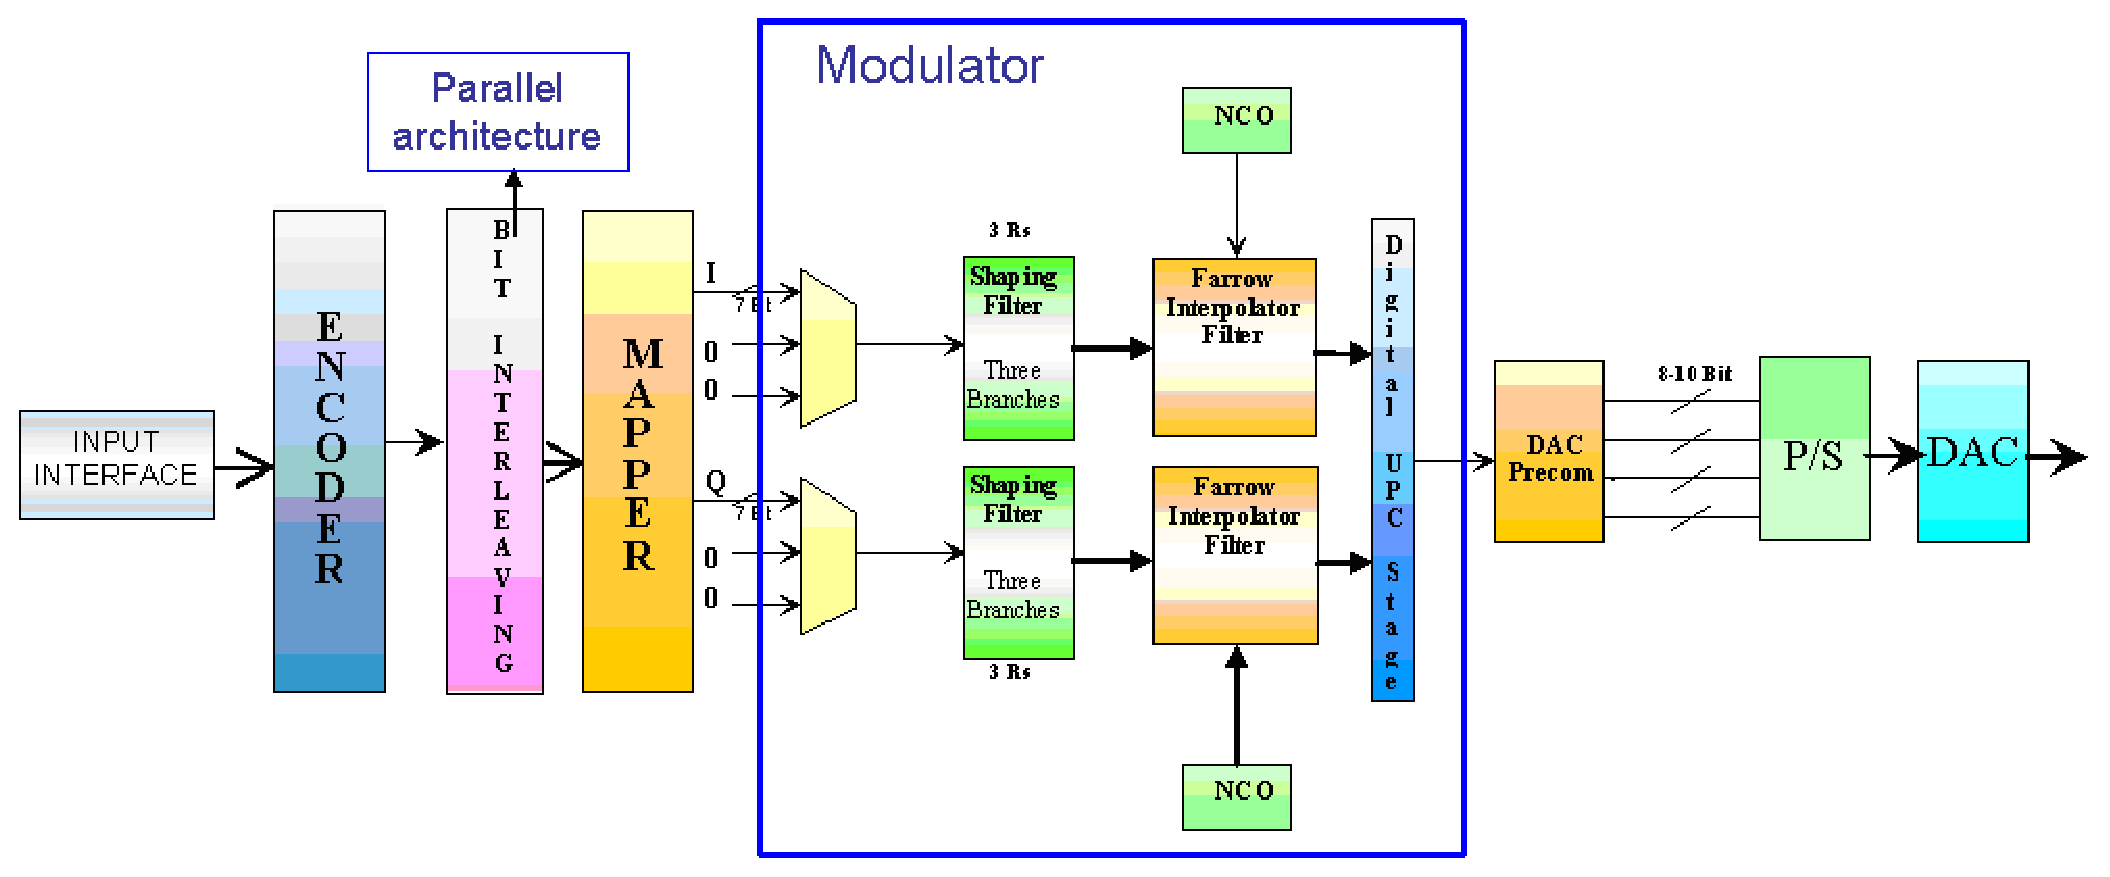
\includegraphics[scale=0.55, angle=90]{TXSection}
\caption{TX Section Architecture}
\label{fig:TXSection}
\end{figure}

\begin{description}
\item[Input Interface] This is the flexible block acquiring the source data: as many packets as required are acquired  depending on the output symbol rate, modulation and coding rate of the PLFRAME to be generated.

\item[DVB-S2 Formatter] As described in chapter \ref{ch:DVBS2Arch&Conc}, this block composes the frame. The DVB-S2 normal FEC-frame has a fixed length of 64800 bits, excluding pilot bits insertion.

\item[Base Band Header Insertion] This block inserts a fixed length Baseband Header (BBHEADER) of 10 bytes shall be inserted in front of the DATA FIELD, describing its format (the maximum efficiency loss introduced by the BBHEADER is 0,25\% for \(n\ped{ldpc}=64800\) and 1\% for \(n\ped{ldpc}=16200\), assuming that inner code rate is \(1/2\). As said in chapter 2, Data field is simply constituted by the information bits; finally, zero-bits shall be appended after this field in order to have a constant length of \(k\ped{bch}\) bits (Padding).

\item[BB Scrambling] This block is necessary since the complete BBFRAME shall be randomized. The randomization sequence shall be synchronous with the BB\-FRAME, starting from the MSB and ending after \(k\ped{bch}\) bits. The randomization is realized by adding the BBFRAME sequence (starting from MSB) to a random sequence generated by a linear shift register and initialized at the beginning of each frame. The scrambling sequence has been stored in a ROM memory; informative bits are processed in parallel by means of a standard parallelization of a linear system.

\item[Physical Layer Scrambling Block] Prior to modulation, each PLFRAME, excluding the PLHEADER, has to be randomized for energy dispersal by multiplying the \((I+ \im Q)\) samples by a complex randomization sequence \((CI+ \im CQ)\). The randomization sequence is re-initialized at the end of each PLHEADER, besides the PLFRAME duration depends on the modulation selected, thus the randomization sequence length shall be truncated to the current PLFRAME length. The scrambling code sequences are constructed by combining two real \(m\)-sequences (generated by means of two generator polynomials of degree 18) into a complex sequence. The resulting sequences thus constitute segments of a set of \emph{Gold sequences}. The physical layer scrambling has been generated by a ROM memory which is read starting from the address 0 at the beginning of each frame.

\item[Encoder Block] This functional block provides the following functions:
    \begin{itemize}
    \item 	CRC-8 (1-Byte Cyclic Redundancy Check) insertion on the incoming packets;
    \item outer (BCH) and inner (LDPC) encoding, according to the selected coding rate (see \tbref{tb:codpar});
    \item bit interleaving, when the selected modulation format is an 8PSK.
    \end{itemize}

\item[CRC-8 Encoder] This functional block is necessary only for packetized streams only.

\item[Bit Interleaving Block] The direct implementation of the Bit Interleaving suggested by Hughes Network Systems (HNS) in the ETSI standard definition strongly reduces the maximum achievable baud rate; in effect maximum baud rate is \(f\ped{ck}/\eta\), where \(f\ped{ck}\) is the operating frequency and \(\eta\) is the modulation efficiency.

    Later on an alternative parallel architecture is introduced that doesn't present this limitation.

    Our goal has been to carry out a parallel bit interleaving by means of a block that outputs one modulation signal per clock cycle in order to maximize the achievable baud rate. In this case, if \(f\ped{ck}\) [MHz] is the operating frequency, we will have a maximum achievable baud rate equal to \(f\ped{ck}\) [MBaud].

    The goal is obtained by means of a parallel architecture, which allows to read \(\eta\) consecutive bits per clock cycle belonging to different symbols; in this way, we provide one symbol per clock cycle.

\item[Mapper Block] Mapping into constellation is carried out according to the selected modulation format (Q-PSK or 8-PSK); constellations are stored in a ROM (Read Only Memory) and a 7-bit representation has been used for \(I\) and \(Q\) components.

\item[Shaping Filter] The \(I\) and \(Q\) data paths at the output of the serial to parallel block are processed by the SRRC (Squared Root Raised Cosine) filter and polyphase interpolator included on the same structure.

    This filter is used to provide the interpolation and pulse shaping of the data in order to minimize intersymbol interference. The complex valued coded symbols stream is applied at the input of this sub-unit which performs SRRC pulse shaping by a FIR filter running at rate \(3 R\ped s\) . The choice of a processing rate equal to \(3 R\ped s\) is made considering that the desired sampling frequency  \(f\ped{SA}\) is achieved by interpolating the shaped signal; as a consequence an adequate attenuation of the signal spectrum replica, centered around the interpolator input sampling frequency, is required.
%obtained at the DDPU output,
\item[Interpolator Section] In this specific case a third order Farrow Interpolator block has been used to change the rate at the output of the polyphase filter, depending on the input bit rate selected.

\item[Digital Up Conversion (UPC) Stage] This block realizes the up-conversion from the baseband frequency to the intermediate frequency.

\item[DAC Precompensation Filter] This block has been designed to compensate the signal distortion (about \(4\unit{dB}\) from DC to half the sampling frequency) introduced by the D/A conversion; in order to correct this linear distortion a FIR filter is used, just before the DAC.

    This is most for a number of reasons, e.g. the need for complex filter coefficients in case compensation were done at base-band; however, high speed operations are actually desirable: hence, a coefficient simplification is introduced to avoid multiplications and the transpose form of a FIR filter has been used; pipelining can also be used for it to further enhance speed if required.

\end{description}

\clearpage

\section{Test Objectives and Setup}

Aim of this test campaign is to verify the encoder and modulator design and its performances in terms of constellation implementation quality: this is pursued via a statistical characterization on phase and magnitude error.

All tests have been performed after synthesizing the VHDL-based design onto a Stratix II DSP Development Board, which includes an EP2S180 device. Additionally, this board provides two 14-bit D/A converters with an up to 165-Megasample per second rate and single-ended output.

In order to best evaluate the modulator performances, signal at the output of D/A converter has been routed to an ultra-broadband Vector Signal Analyzer (VSA) which also executes demodulation. The VSA is composed by the association of:

\begin{enumerate}

\item a MSO6054A 6000 series oscilloscope (\(500\unit{MHz}\) bandwidth, \(4\unit{Gsa/s}\));

\item the 89601A vector signal analyzer software, running onto a PC interconnected to the oscilloscope via an Ethernet port.

\end{enumerate}

Test setup equipments is shown in \figref{fig:TestEqu}, Stratix II FPGA hosts the VHDL-based design.

\begin{figure} \centering
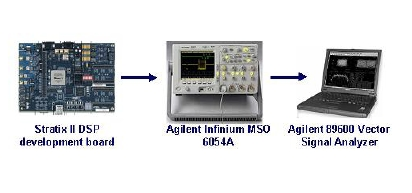
\includegraphics[scale=.8]{te1}
\caption{Laboratory Test} \label{fig:TestEqu}
\end{figure}

In particular, sampling rate and IF center frequency have been designed in order to meet the requirements in presence of the HW constraints imposed by both the prototyping board and the anti-image filters available. A parallel to serial converter at the output of modulator has been added to serialize the four parallel data streams at the output of Tx section. Note that the four parallel flows are normally necessary to relax the high speed as well as the relevant criticality in the transfer of data from the TX DSP section to the DAC. The overall transmitter schematic diagram is shown in figure above.

Tx section performances have been evaluated in terms of constellation quality, furthermore, a statistical analysis of magnitude and phase errors has been computed exploiting the dedicated tool available in VSA.

The tool is based on the EVM (Error Vector Magnitude) analysis. EVM is the Root Mean Square (RMS) of the error vectors computed and expressed as a percentage of the square root of the mean power of the ideal signal. The instrument, apart from peak values, can also provide the statistically estimated standard deviation of the EVM and of the phase error.

The error vector is the magnitude of the vector, at the detected symbol location, which connects the I/Q reference-signal phasor to the I/Q measured-signal phasor, and is computed as follows (for a graphical representation refer to the phasor diagram shown below):
\begin{equation}
\mathrm{EVM}[n] = \sqrt{{I\ped{err}[n]}^2 + {Q\ped{err}[n]}^2}
\end{equation}
where the variable \(n\) indicates the discrete symbol time and obviously the error in phase is \(I\ped{err} = I\ped{Ref}-I\ped{Meas}\), that is, the reference \(I\) component is subtracted to the measured component.
In a similar way the component of error in quadrature can be measured as follow: \(Q\ped{err} = Q\ped{Ref}-Q\ped{Meas}\).

\begin{figure} \centering
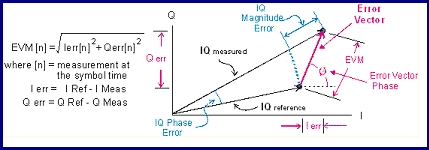
\includegraphics[scale=.8]{EVMAGN}
\caption{Error vector magnitude computation} \label{fig:EVMAGN}
\end{figure}

In addition, magnitude error and phase error (computed as described in \figref{fig:MAGNPHASE}) vs time diagram (expressed in symbols) have been plotted to better evaluate constellation quality.

\begin{figure} \centering
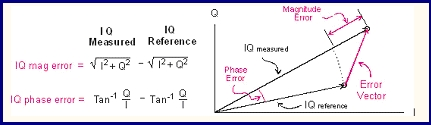
\includegraphics[scale=.8]{MAGNPHASE}
\caption{Magnitude and phase error computation} \label{fig:MAGNPHASE}
\end{figure}

\clearpage

\section{Test Results}

In this preliminary test campaign, some measurements on the developed DVB-S2 TX section have been performed. For both \(2 \unit{MBaud}\) and \(30 \unit{MBaud}\) symbol rates, demodulated signal constellations have been plotted.

From a statistical point of view, modulator performance have been evaluated computing phase and magnitude error in the way indicated before.

From results of these preliminary test, degradation due to imperfect image rejection and DAC distortion is clear.

\subsection{2 MBaud --- 16 APSK}

In this test, signal constellation demodulated by VSA has been visually and qualitatively analyzed. In addition, phase and magnitude error have been plotted and quantified via statistical measurements to better analyze the modulation quality.

\begin{figure} \centering
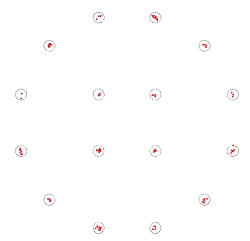
\includegraphics[scale=1.2]{2MBaud16APSK2}
\caption{2MBaud 16 APSK constellation} \label{fig:16PSK2MBaud}
\end{figure}

The statistical analysis of errors leads to the following results:

\begin{center}\begin{tabular}{||p{4.22cm}||p{4.03cm}||}
\hline
 \multicolumn{1}{|p{4.22cm}|}{\centering EVM} &  \multicolumn{1}{p{4.03cm}|}{\centering 2\%} \\
 \multicolumn{1}{|p{4.22cm}|}{\centering Magnitude Error} &  \multicolumn{1}{p{4.03cm}|}{\centering 0,9\%} \\
 \multicolumn{1}{|p{4.22cm}|}{\centering Phase Error} &  \multicolumn{1}{p{4.03cm}|}{\centering 3 deg} \\
\hline
\end{tabular}\end{center}
A very limited degradation with respect to the ideal constellation is actually evident.
%\begin{figure} \centering
%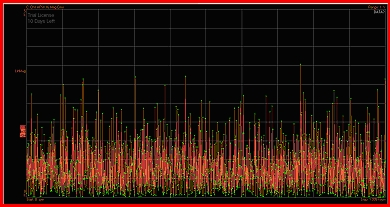
\includegraphics[scale=0.8]{IQerr}
%\caption{\(I\)-\(Q\) Magnitude Error (16-APSK --- 2 MBaud)}
%\end{figure}

%\begin{figure} \centering
%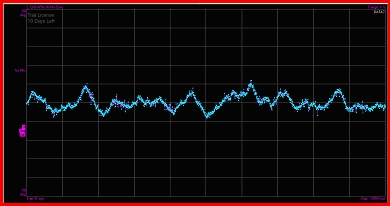
\includegraphics[scale=0.8]{IQPHA16APSK}
%\caption{\(I\)-\(Q\) Phase Error (16-APSK --- 2 MBaud)}
%\end{figure}

\begin{figure} \centering
\subfloat[Signal Spectrum]{
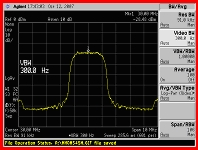
\includegraphics[scale=.8]{Spectrum16APSK2MB}
} \qquad
\subfloat[Replica Distance]{
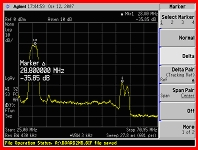
\includegraphics[scale=.8]{SpectrRepl2MB}
}
\caption{\(2 \unit{MBaud}\) 16-APSK Signal spectra} \label{fig:SigReplica}
\end{figure}

\clearpage

\subsection{30 MBaud --- 8 PSK}

In this test, degradation of modulator performances due to the absence of a DAC pre-compensation filter is clear. In following figures a less scattered plot with pre-compensation filter can be seen.

\begin{figure} \centering
\subfloat[Signal constellation quality in presence of DAC compensation]{
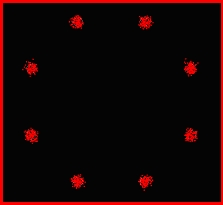
\includegraphics[scale=.8]{8PSKConst}
} \qquad
\subfloat[Signal constellation quality in absence of DAC compensation]{
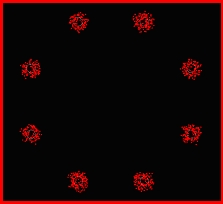
\includegraphics[scale=.8]{8PSKConstNDAC} \label{fig:noDAC}
} %\qquad
%\subfloat[Signal constellation quality in presence of DAC compensation]{
%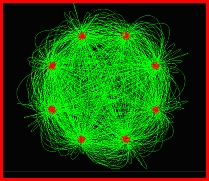
\includegraphics[scale=.8]{8PSKdac}
%} \qquad
%\subfloat[Signal constellation quality in absence of DAC compensation]{
%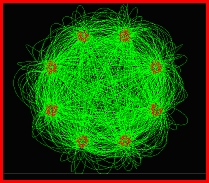
\includegraphics[scale=.8]{8PSKnodac}
%}
\caption{\(30 \unit{MBaud}\) 8-PSK Scatter Plots} \label{fig:8PSK30MBaud}
\end{figure}

Signal spectra comparison in \figref{fig:SpectrComp} shows the distortion introduced by the DAC: the blue curve, as a matter of fact, is the no-precompensated signal spectrum, which results in a very scattered constellation (\figref{fig:noDAC}); the yellow one, representing the signal spectrum of the same signal processed by the precompensation filter, results in a better scatter plot.

\begin{figure} \centering
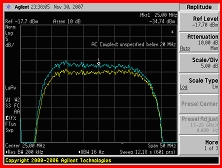
\includegraphics[scale=1.3]{DACvsNDAC}
\caption{Spectra comparison between the spectrum of the signal precompensated (yellow one) and that of the signal non-precompensated (blue one)} \label{fig:SpectrComp}
\end{figure}


The statistical analysis of errors leads to the following results:
\begin{center}\begin{tabular}{||p{3.13cm}||p{4.91cm}p{4.78cm}||}
\hline
 \multicolumn{1}{|p{3.13cm}|}{\centering} &  \multicolumn{1}{p{4.91cm}}{\centering Without pre-compensation filter} &  \multicolumn{1}{p{4.78cm}|}{\centering With pre-compensation filter} \\
\hline
 \multicolumn{1}{|p{3.13cm}|}{\centering EVM} &  \multicolumn{1}{p{4.91cm}}{\centering 9\%} &  \multicolumn{1}{p{4.78cm}|}{\centering 4\%} \\
 \multicolumn{1}{|p{3.13cm}|}{\centering Magnitude Error} &  \multicolumn{1}{p{4.91cm}}{\centering 6\%} &  \multicolumn{1}{p{4.78cm}|}{\centering 2\%} \\
 \multicolumn{1}{|p{3.13cm}|}{\centering Phase Error} &  \multicolumn{1}{p{4.91cm}}{\centering 3 deg} &  \multicolumn{1}{p{4.78cm}|}{\centering 1,5 deg} \\
\hline
\end{tabular}\end{center}



%\begin{figure} \centering
%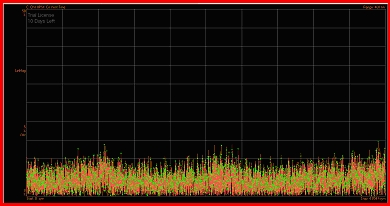
\includegraphics[scale=.8]{IQMagn8PSK}
%\caption{I-Q Magnitude Error (30 MBaud 8-PSK)}
%\end{figure}

%\begin{figure} \centering
%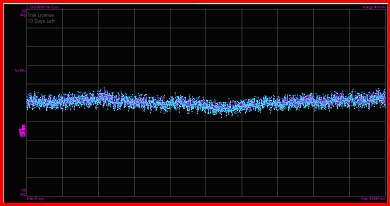
\includegraphics[scale=.8]{IQPha8PSK}
%\caption{I-Q Phase Error (30 MBaud 8-PSK)}
%\end{figure}

\clearpage

\subsection{30 MBaud --- 16 APSK}

In this test, signal constellation demodulated by VSA has been visually and qualitatively analyzed. In addition, phase and magnitude error have been plotted and quantified via statistical measurements to better analyze the modulation quality.


\begin{figure} \centering
\subfloat[Scatter]{
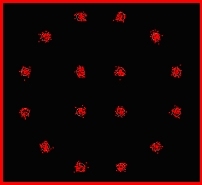
\includegraphics[scale=.8]{16APSKSca1}
} \qquad
\subfloat[Scatter]{
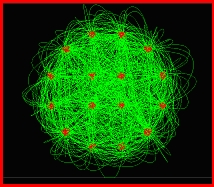
\includegraphics[scale=.8]{16APSKSca2}
} \caption{\(30 \unit{MBaud}\) 16-APSK Scatter Plots} \label{fig:16APSK30MBaud}
\end{figure}

The statistical analysis of errors leads to the following results:
\begin{center}\begin{tabular}{||p{4.22cm}||p{4.03cm}||}
\hline
 \multicolumn{1}{|p{4.22cm}|}{\centering EVM} &  \multicolumn{1}{p{4.03cm}|}{\centering 3\%} \\
 \multicolumn{1}{|p{4.22cm}|}{\centering Magnitude Error} &  \multicolumn{1}{p{4.03cm}|}{\centering 1,5\%} \\
 \multicolumn{1}{|p{4.22cm}|}{\centering Phase Error} &  \multicolumn{1}{p{4.03cm}|}{\centering 2 deg} \\
\hline
\end{tabular}\end{center}


%\begin{figure} \centering
%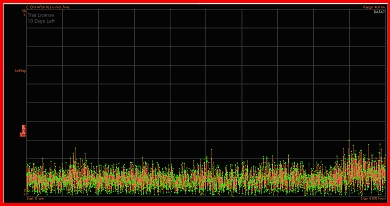
\includegraphics[scale=.8]{IQMagn1630MB}
%\caption{I-Q Magnitude Error (30 MBaud 16-APSK)}
%\end{figure}

%\begin{figure} \centering
%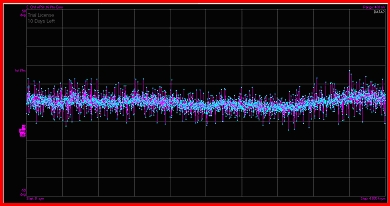
\includegraphics[scale=.8]{IQPha1630MB}
%\caption{I-Q Phase Error (30 MBaud} 16-APSK)}
%\end{figure}

\clearpage

\section{64-APSK Modulator}

The modulator tested by TAS can also provide modulations of higher order with respect to DVB-S2 (e.g. MHOMS modulation schemes). Figure shows a progressive expansion of time-scale representation for a 64-APSK modulation scheme, being this the most innovative modulation, and the four signal envelope level either(points lie on 4 concentric circumferences, that is, each radius represents the amplitude of each level provided).


\begin{figure} \centering
\subfloat[]{
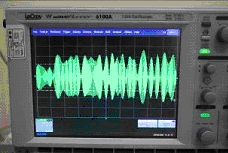
\includegraphics[scale=.8]{64APSK1}
} \qquad
\subfloat[]{
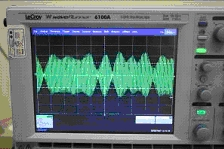
\includegraphics[scale=.8]{64APSK2}
} \qquad
\subfloat[]{
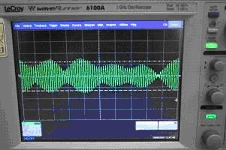
\includegraphics[scale=.8]{64APSK3}
} \qquad
\subfloat[]{
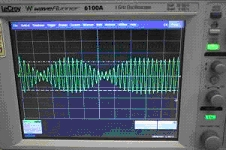
\includegraphics[scale=.8]{64APSK4}
}
\caption{64-APSK Signal} \label{fig:64APSKwvform}
\end{figure}

\chapter{Conclusions} \label{ch:Conclusions}

In this thesis we have dealt with a digital communications TX section which can provide a reliable information transmission via satellite while complying with the challenging requirements on performance imposed by DVB-S2 standard.

My most working contributions to the overall project of the DVB-S2 TX section developed by TAS-I have been focused specifically on
\begin{itemize}
\item study of the theory underlying the BCH code: Galois fields and cyclic codes theory in order to have the theoretical basis to understand the DVB-S2 code structure and analyze algorithms related to;
\item theoretical analysis of DVB-S2 BCH code structure from which we have reach the conclusion that the DVB-S2 outer code (BCH) must be \emph{primitive} and \emph{shortened};
\item study of the BCH encoding procedures and algorithms and its related (serial) architectures;
\item modelling and design of a parallel BCH encoder with an high degree of parallelism in order to best match the TX Section (developed by TAS) speed requirements;
\item development of a Berlekamp-Massey software decoder in order give a proof of the error correction capacity of the code (encoder); to this purpose we have defined specifical routines aimed to compute arithmetic tables useful in decoding and error detection computations;
\item development of a software package (C/C++) in order to verify the functioning of architectures envisaged and give support to VLSI designers in validation of the correspondent VHDL model;
\end{itemize}

Concerning to the DVB-S2 architecture and overall TX section and thanks to the contribution of the TAS-I Algorithm \& Architectures team, this thesis has dealt with:
\begin{itemize}
\item identification of the strategic importance of satellite communications in some application scenarios such as Multimedia, Earth observation, radio-localization and navigation, \emph{etc.};
\item review of novel techniques aimed at obtaining top performance by handling modulation and coding schemes jointly;
\item assessment of the features of ACM techniques, which allow to better utilization of resources onboard while ensuring an high QoS (Quality of Service);
\item design of the DVB-S2 Modem architecture and blocks focusing on concatenated coding (BCH-LDPC) and modulation schemes;
\item qualitative description of LDPC encoding/decoding algorithms, and on the latter we have highlighted the importance of the BCH code to counteract against error floors affecting LDPC \emph{iterative decodings};
\item BCH encoding procedures and algorithms and its related (serial) architectures;
\item modelling and design of a parallel encoder with an high degree of parallelism in order to best match the TX Section (developed by TAS-I) speed requirements;
\item selection between two possible (and functionally equivalent) BCH parallel architectures in order to work in ACM;
\item development of a Berlekamp-Massey software decoder in order give a proof of the error correction capacity of the code (encoder); to this purpose we have defined specifical routines aimed to compute arithmetic tables useful in decoding and error detection computations;
\item development of a software package (C/C++) in order to verify the functioning of architectures envisaged and give support to VLSI designers in validation of the correspondent VHDL model;
\item participation to a preliminary laboratory test and validation of the TAS-I developed DVB-S2 TX section  .
\end{itemize}
%Before the equipment production, the work in progress will be devoted to
%\begin{itemize}
%\item evaluate and thus analyze BER curves by simulations
%\item measurement and BER analysis by a commercial BER meter
%\item compare BERs obtained by the BER meter with those theoretically expected
%\end{itemize}


\appendix
\include{basic}


\bibliography{thesis}

\nocite{*}








\end{document} 